% !TEX root = ../main.tex
%
% Copyright 2015
% Jérémy Levallois <jeremy.levallois@gmail.com>
%
% This file and related figures are under Creative Commons CC BY-NC-SA 4.0
% See <https://creativecommons.org/licenses/by-nc-sa/4.0/>
%
\chapter{Applications}
\label{sec:applications}

% \cleanchapterquote{We have seen that computer programming is an art, because it
% applies accumulated knowledge to the world, because it requires skill and
% ingenuity, and especially because it produces objects of beauty.}{Jean-Claude
% Vandamme}{Ma vie, mon œuvre.}

\setcounter{minitocdepth}{3}
\minitoc

\newpage

% \begin{table}[h]
% \begin{tabular}{@{}p{2cm}lp{2cm}p{8cm}@{}}
% \toprule
% \multicolumn{4}{c}{\textsc{À citer}} \\ \midrule
% SUSAN2D & \cite{SUSAN2D} & intersection volume; image; 2D     & Détection de singularités à base de volume de l'intersection \\
% SUSAN3D & \cite{SUSAN3D} & \emph{à lire} & Variante 3D de SUSAN \\
% Witkin1983 & \cite{Witkin1983} & \emph{\#FIRST} & Première mention d'espace d'échelle \\
% Pottmann2006 & \cite{Yang2006} & feature & Ils font un seuil sur le max des k1 k2. \\
%
% \bottomrule
% \end{tabular}
% \end{table}
% \newpage

Dans ce chapitre, nous nous intéressons aux applications des estimateurs
locaux introduits dans le \RefChapitreN{sec:estimators}. Dans un premier temps,
nous détaillons une méthode d'extraction de singularités («
\anglais{features} ») à partir de formes 2D et 3D
(\RefSection{sec:applications:feature}). Ces
travaux ont été publiés dans \cite{SMI2015}.
%
 % pour ensuite nous plonger dans la reconstruction de surfaces
 % (\RefSection{sec:applications:reconstruction}).
%
Nous verrons ensuite le lien entre les travaux présentés dans cette thèse et le
projet \textsc{digitalSnow} auquel nous avons contribué. Enfin, nous parlerons
de l'implémentation de ces travaux au sein de la bibliothèque open-source de
géométrie digitale \textsc{DGtal} \cite{DGtal}
(\RefSection{sec:applications:dgtal}).

\section{Estimation de singularités}%
\label{sec:applications:feature}

%\subsection{Introduction}
%
L'extraction de points caractéristiques sur des formes géométriques apparaît
comme essentiel depuis plusieurs années. Il existe bon nombre d'applications les
utilisant, allant de la reconnaissance d'objets dans une scène \cite{Brown2005} à la compression
de données \cite{Peng2010}, l'analyse de données médicales \cite{Lannister1996}
ou bien archéologiques \cite{Mellado2013}. Plus récemment, la rapide
démocratisation de systèmes d'acquisition 3D à bas coût comme la \emph{Microsoft
Kinect} amène un nouveau regain d'intérêt pour l'analyse de formes
\cite{Janoch2013,KinectData}.
%
%% Parler de features globales (aire, volume, moments, D2 shape distributions) et locales ?
%
Dès lors que nous voulons étudier un objet dont on ne connaît pas les propriétés
mathématiques, nous nous intéressons à récupérer des informations permettant de
l'identifier de manière unique. Une information pertinente beaucoup étudiée ces
dernières années est la détection de points caractéristiques. Derrière ce terme
se cachent deux notions : la saillance et les singularités. Les définitions de
ces deux termes ne sont pas clairement établies. Nous allons considérer que la
détection de saillances s'intéresse à récupérer les zones remarquables de
l'objet d'un point de vue perceptif/cognitif (par exemple le nez sur un visage,
les bras et les jambes sur un corps) tandis que la détection de singularités
extrait les discontinuités locales distinguables de son voisinage (par exemple
les rides sur un visage). La première est plutôt une information visuelle alors
que l'autre intègre des informations géométriques de l’objet. Nous nous
intéresserons ici uniquement aux singularités.
%
% C'est là tout le problème lorsqu'on s'intéresse aux \emph{features} : la
% définition varie en fonction des problématiques. Est-ce que c'est une propriété
% qui est distinguable de tous les autres objets, ou bien si c'est une propriété
% qui nous dit quelles parties d'un objet est inhabituel et réclame de l'attention ?
% Nous parlerons ici principalement de saillance visuelle. Est-ce que ce sont des
% parties d'une forme dont la surface n'est pas dérivable (parties non-$C^1$)
% comme le bord d'une table par exemple --- Nous nommerons ceci des singularités
% de la surface ---.
%
% \todoJeremy{search in 3D object databases / face detection}
%%% Research into 3D mesh saliency is largely inspired by corresponding work on 2D images [Itti et al. 1998; Walther and Koch 2006; Hou and Zhang 2007; Goferman et al. 2010]. In particular, the concept of scale space has been successfully extended to the mesh do- main. (papier de Mesh saliency via spectral analysis)
%
%%% HOWARD, I. 2002. Seeing in depth. University of Toronto Press
% In general, estimating saliency in 2D projections of meshes does not sufficiently utilise depth information within the original data, which, as mentioned in [Howard 2002], is a key stimulus for human perception of a static scene.
%
% Il apparaît alors qu'un moyen simple et rapide de les détecter est de seuiller
% la courbure. En effet, nous pouvons facilement voir la relation entre la
% courbure et les zones d’intérêt : les zones de fortes courbures sont
% \emph{généralement} des zones d’intérêts.
%
% \todoJeremy{expliquer singularités non-$C^1$}
%
% \todoJeremy{expliquer l'espace-échelle
% http://www.nada.kth.se/~tony/abstracts/Lin94-SI-abstract.html}
% T. Lindeberg, Scale-Space Theory in Computer Vision, Kluwer Academic Publishers, Norwell, MA, USA, 1994.
%


Nous allons tout d'abord proposer un aperçu des méthodes utilisées dans la
littérature pour extraire les singularités
(\RefSection{sec:applications:feature:SOTA}), puis nous détaillerons notre
méthode basée sur l'analyse de la variation de l'estimateur de courbure par
intégration défini dans le \RefSection{sec:estimators:volume} en fonction de la
géométrie de la forme (\RefSection{sec:applications:feature:II}). Enfin, nous
présenterons une évaluation expérimentale complète de notre estimateur face à
ceux de la littérature (\RefSection{sec:applications:feature:comparison}).
%
\subsection{État de l'art}%
\label{sec:applications:feature:SOTA}
%
Il existe une très vaste littérature sur les problèmes d'extraction de points
caractéristiques sur des formes. Nous avons choisi les méthodes les plus
représentatives de cette littérature afin d'avoir un ensemble complet
d'estimateurs auxquels nous pourrons nous comparer. Nous les avons classés par
catégories : les méthodes « \anglais{Ridges and Valleys} »
(\RefSection{sec:applications:feature:ridge}), les méthodes basées sur un
morceau surfacique (\RefSection{sec:applications:feature:patch}) et les méthodes
d'analyse spectrale (\RefSection{sec:applications:feature:spectral}). Nous
comparerons ces estimateurs dans le
\RefSection{sec:applications:feature:comparison}.
%
\subsubsection{Méthodes « Ridges and Valleys »}%
\label{sec:applications:feature:ridge}
%
Nous souhaitons caractériser les discontinuités du bord d'un objet; une méthode
naturelle est de s'intéresser aux maxima et minima locaux, nommés \respp «
\emph{Ridge} » et « \emph{Valley} » (« Crête » et « Vallée » en français, car
cette notion est assez similaire aux crêtes géographiques).
%
\cauthors{Vergne}{Vergne2011} définissent cela plus formellement :
%
\begin{equation}
  \mathcal{S} = \left\{ \vx \in \R^2 |
  \frac{\delta f(\vx)}{\delta \theta(\vx)} = 0,
  \frac{\delta^2 f(\vx)}{\delta \theta(\vx)^2} < 0 \right\} \,,
\end{equation}
%
où $\mathcal{S} \subset \R^2$, $f$ une fonction de hauteur $C^2$ et $\theta$ une
champ de direction $C^1$. Afin de détecter les maximas et minimas locaux, il
convient de remplacer $f$ et $\theta$ par les valeurs du
\RefTable{tab:ridges-valleys-fonctions}.
%
\begin{table}[h]
  \begin{center}
    %
    \caption{Tableau des fonctions pour détecter les crêtes, les vallées et les
    points d’inflexion d'une surface. $\PrincCurv{max}$ et $\PrincCurv{min}$
    désignent les fonctions donnant les valeurs de la courbure principale
    maximale et minimale au point $\vx$, $\PrincDir{max}$ et $\PrincDir{min}$ les fonctions
    donnant les directions de courbure maximale et minimale $\vx$, et $\vv_{max}$ la
    fonction donnant la valeur du gradient de courbure $\vx$.}
    %
    \label{tab:ridges-valleys-fonctions}
    \begin{tabular}{@{}lrr@{}}
      \toprule
                                          & $f(\vx)$            & $\theta(\vx)$           \\ \midrule
      Crêtes de la surface                & $\PrincCurv{max}(\vx)$   & $\PrincDir{max}(\vx)$        \\
      Vallées de la surface               & $-\PrincCurv{min}(\vx)$  & $\PrincDir{min}(\vx)$        \\
      Points d’inflexion de la surface  & $|\vv_{max}(\vx)|$       & $\vv_{max}(\vx)/|\vv_{max}(\vx)|$ \\ \bottomrule
    \end{tabular}
  \end{center}
\end{table}
%
Dans ce contexte, les discontinuités sont déduites de quantités différentielles
d'ordre $3$ en s'intéressant aux variations des directions principales de
courbure dans un voisinage de la surface \cite{Lai2007,Yang2006}. En seuillant
les déviations angulaire significatives des directions principales de courbure,
nous pouvons alors détecter les discontinuités.

\begin{figure}[ht]{
    \begin{center}
    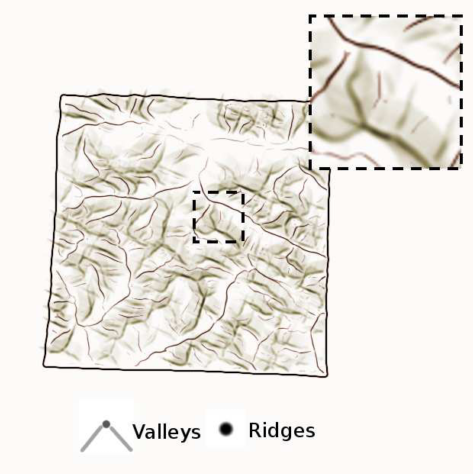
\includegraphics[height=10cm]{images/Feature/RidgesValleys}
    \end{center}}
    \caption[Notations.]{« Crêtes » et « Vallées » (Figure~12 de \cite{Vergne2011}).
      \label{fig:ridges-valleys}}
\end{figure}

Ces techniques amènent une approche formelle à l'extraction de discontinuités,
mais sont dépendantes de l'échelle à travers le seuillage. De plus, elles
nécessitent d'avoir une estimation robuste de quantités différentielles d'ordre
$3$. Lorsque la forme d'entrée est bruitée, ou dans le cadre de données
digitales, ces approches ne s'avèrent pas pertinentes.
%
%
% \subsubsection{Méthodes basées courbure}
% \label{sec:applications:feature:courbure}
% \paragraph{Curvature-based approach for multi-scale feature extraction from 3D meshes and unstructured point clouds \cite{Ho2009}}
%
% \begin{algorithm}[H]
%  \KwData{$P = \{\mathbf{p}_i \in \R^3\}$: set of 3D points sampled from the surface.
% $R = \{r_k\}$: a set of scales.}
%  %\KwResult{nope}
%  \For{$r \in \{r_k\}$}
%  {
%   \For{$\mathbf{p} \in \{\mathbf{p}_i\}$}
%   {
%     Find the neighbourhood $N_r$ at scale $r$\\
%     Fit a jet to $N_r$\\
%     Compute principal curvatures $\PrincCurv{1}$ and $\PrincCurv{2}$\\
%     Compute the curvedness $\mathcal{C}_p$
%       \begin{equation}
%       \begin{center}
%         \mathcal{C}_p = \sqrt{(\PrincCurv{1} \time \PrincCurv{1}) + (\PrincCurv{2}\time \PrincCurv{2}) / 2}
%       \end{center}
%       \end{equation}
%   }
%   Keypoints are positions $\mathbf{p}$ having extremum values $\mathcal{C}_p$ both in the neighbourhood of radius $r_k$ as well as over the above and below scales $(r_{k-1}, r_{k+1})$.
% }
%  \caption{Test}
% \end{algorithm}
%
\subsubsection{Méthodes basées sur un voisinage surfacique}%
\label{sec:applications:feature:patch}
%
Lorsque nous traitons les maillages ou les nuages de points, beaucoup
d'approches se basent sur des quantités calculées par intégration sur des
voisinages de la surface. La caractéristique est déterminée en fonction d'un
score évalué sur la géométrie de voisinages surfaciques centrés autour du point à
considérer. Généralement, les voisinages sont simplement issus d'un noyau
sphérique.
%  Nous allons en détailler quelques-unes
% \cite{Pauly2003,Telea2004} utilisant l'Analyse en Composante Principale
% (\emph{ACP}) sur le voisinage du point d’intérêt. Un score de zone
% caractéristique est alors déterminé grâce à un seuillage, ou grâce au
% comportement du score comme fonction de la taille du voisinage analysé.
% %
% \\
% %
% D'autres \cite{Merigot2011} étendent cette approche pour considérer les matrices
% de covariances de cellules de Voronoï convoluées (\VCMM ou \VCM). En seuillant
% le ratio des valeurs propres du \VCM, nous obtenons une extraction robuste des
% singularités sur un nuage de points ou sur un maillage.
% %
% \\
% %


Certaines approches produisent des résultats pour une échelle donnée (pour une
taille de voisinage fixée). Toutefois, les techniques récentes s'intéressent à
analyser la forme à plusieurs échelles, permettant d'en extraire des
informations de toutes tailles. Ces approches sont nommées « des méthodes en
espace d'échelle » \cite{Witkin1983} (« \anglais{Scale-space} »), avec
généralement la taille du voisinage comme paramètre.
%
\paragraph{Valeurs propres de la matrice de covariance}
%
\cauthors{Pauly}{Pauly2003} utilisent les valeurs propres de la matrice de
covariance $J$ calculée en chaque point $\vx \in \dS$ de la surface de la forme
$\Shape \subset \R^3$ pour un voisinage donné. Ils exploitent les trois valeurs
propres $\lambda_0 \leq \lambda_1 \leq \lambda_2$ de cette matrice afin
d'obtenir une valeur de variation de surface (introduite dans \cite{Pauly2002})
en fonction d'un ensemble de rayons $\{ R_i \}_{0 \le i \le n}$ :
%
\begin{equation}
  \tau_{R_i}(\vx) \EqDef \frac{\lambda_0(J_{R_i}(\vx))}{\lambda_0(J_{R_i}(\vx)) + \lambda_1(J_{R_i}(\vx)) + \lambda_2(J_{R_i}(\vx))} \,.
\end{equation}

\begin{figure}[ht]{
  \begin{center}
    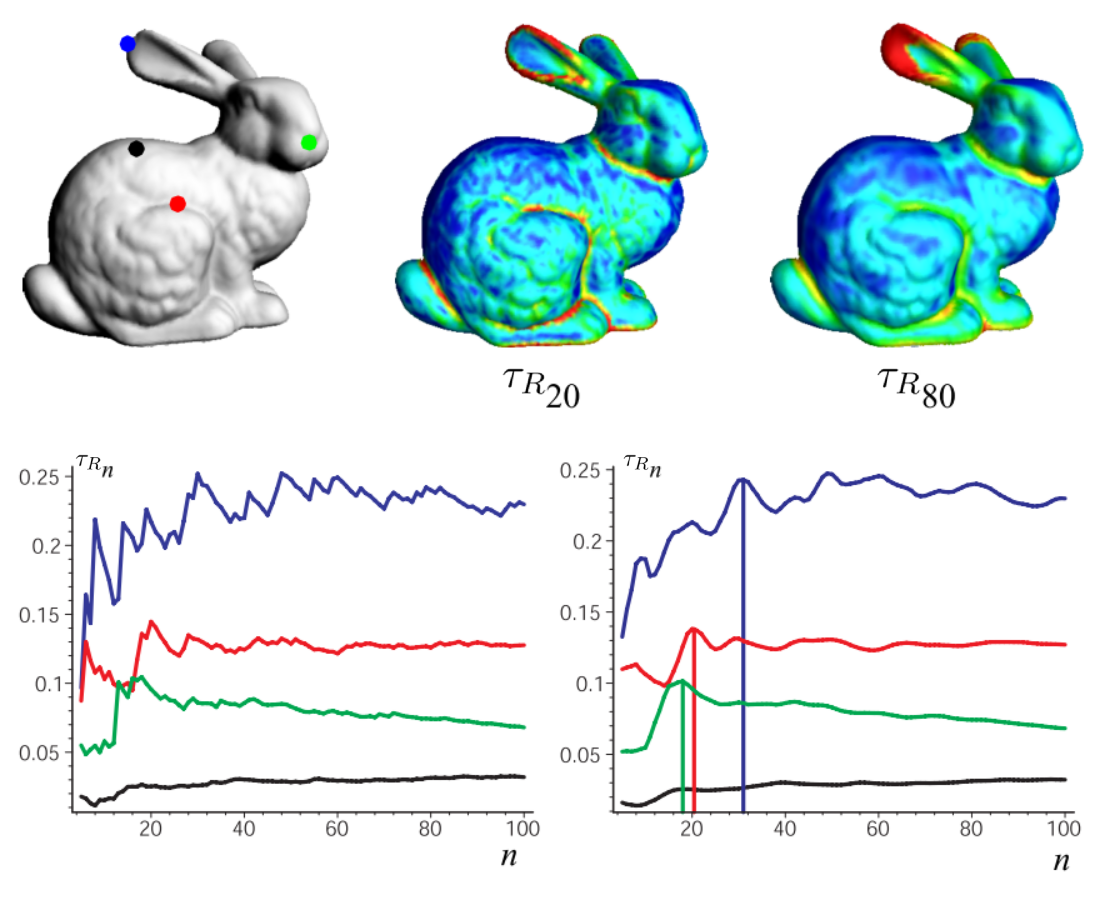
\includegraphics[height=10cm]{images/Feature/PaulyTau}
  \end{center}}
    \caption[Valeurs retournées par $\tau_{R_i}$.]{Valeurs retournées par $\tau_{R_i}$ (Figure~7 de \cite{Pauly2003}).
    \label{fig:pauly-tau}}
\end{figure}

Puisque les valeurs propres diminuent lorsque la courbure augmente, il apparaît
que la valeur de $\tau_{R_i}$ sera plus grande sur les singularités que sur les parties
à courbure nulle de la surface. Pour appuyer cette distinction, les auteurs calculent un
poids sur chaque point : pour tous les rayons, le poids est incrémenté à chaque
fois que $\tau_{R_i}$ est supérieur à un seuil $\tau_{max}$ défini par
l'utilisateur. Plus formellement :
%
\begin{equation}
  \label{eq:pauly-omega}
  \omega(\vx) \EqDef Card \{ \tau_{R_i}(\vx) \geq \tau_{max}\,|\,0\leq i < n \} \,.
\end{equation}
%
Il est alors évident que le poids sera plus important sur les zones
angulaires (de couleur jaune sur la \RefFigure{fig:pauly-cubesphere})
tandis qu'il sera faible sur le reste de la forme (en bleu).

\begin{figure}[ht]{
  \begin{center}
    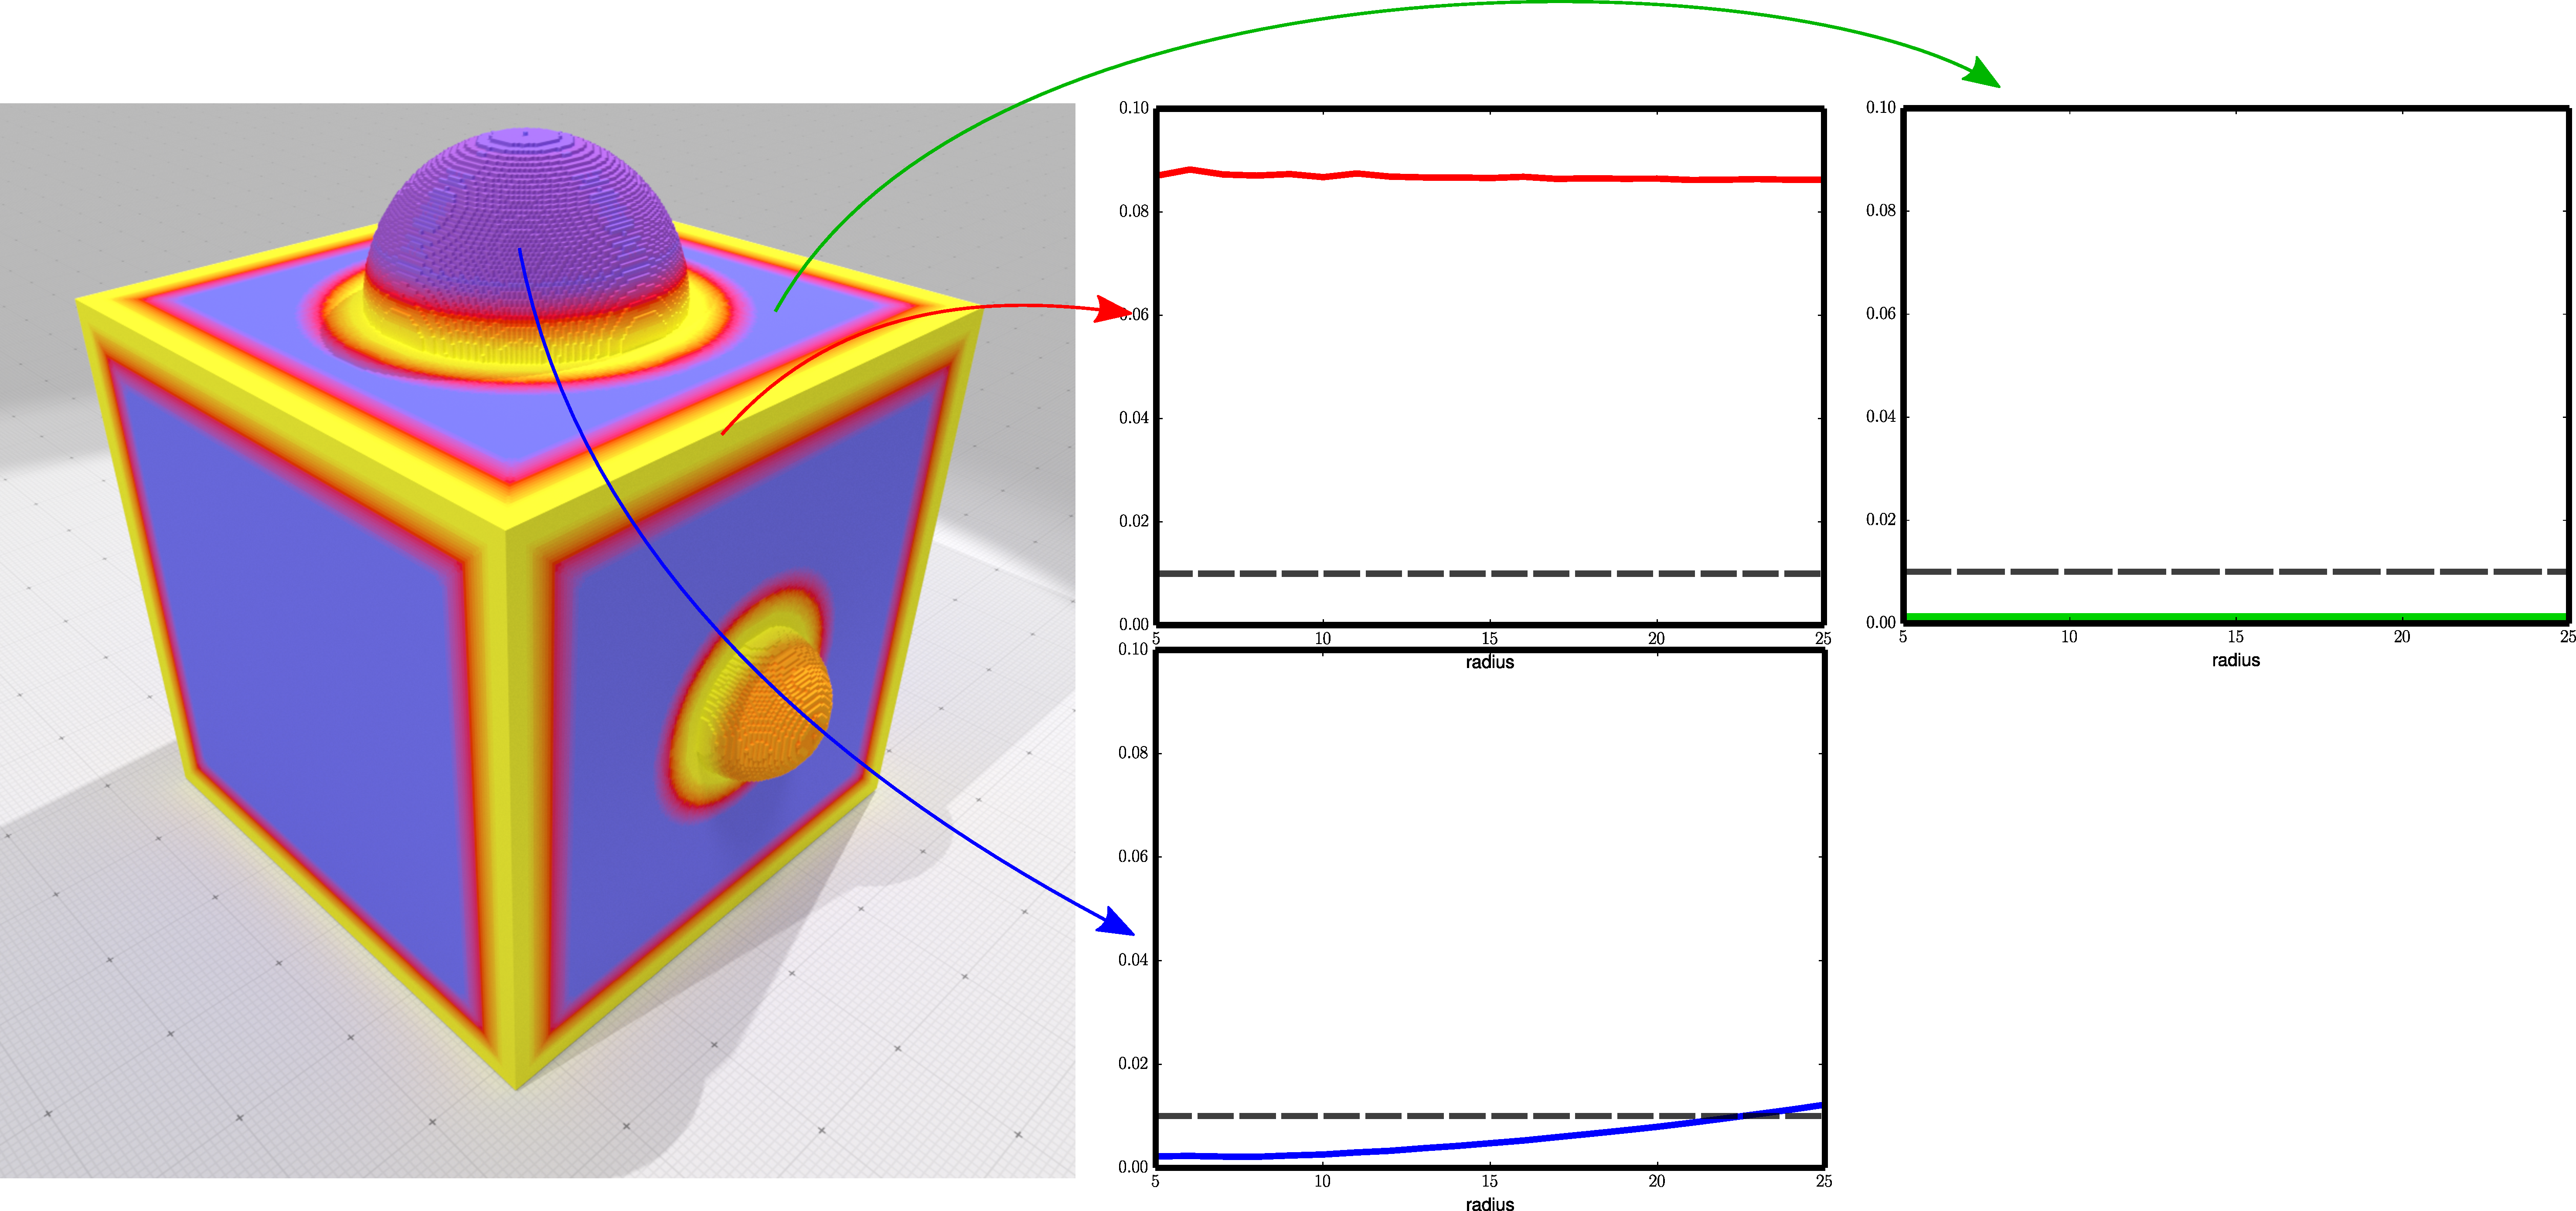
\includegraphics[height=6.8cm]{figures/CubeSpherePlotPauly}
  \end{center}}
    \caption[Résultat de l'\RefEquation{eq:pauly-omega}]{Résultat de l'\RefEquation{eq:pauly-omega} avec comme paramètres $\tau_{max} = 0.01$, $5 \le i \le 25$.
    \label{fig:pauly-cubesphere}}
\end{figure}

Puisque ce détecteur est relié à la variation de la surface, il fournit des
résultats géométriquement valides. Cependant, cela nécessite que l'utilisateur
fournisse un paramètre $\tau_{max}$ qui dépend de la géométrie de la forme : il
peut considérer des petites parties lisses comme des zones caractéristiques si
$\tau_{max}$ est choisi trop petit. C'est ce que nous voyons sur la
\RefFigure{fig:pauly-cubesphere} avec la petite sphère sur la face verticale.
Également, puisque ce détecteur se base sur des informations surfaciques, il est
assez sensible au bruit comme nous le verrons plus tard dans le
\RefSection{sec:applications:feature:comparison}.
%
\paragraph{Variation de barycentre}
%
\cauthors{Clarenz}{Telea2004} définissent quant à eux un critère de
classification de surface basé sur la variation du barycentre $\vb$ et de la
matrice de covariance\footnote{Dans \cite{Telea2004}, les auteurs nomment le
moment d'ordre zéro comme le barycentre et le moment d'ordre un comme la matrice
de covariance, ce qui peut porter à confusion avec notre définition des moments
vue dans le \RefSection{sec:moments-geo}.} de morceaux surfaciques
$\Ball{R}{\vx} \cap \dS$.

\begin{figure}[ht]
  \begin{center}
    
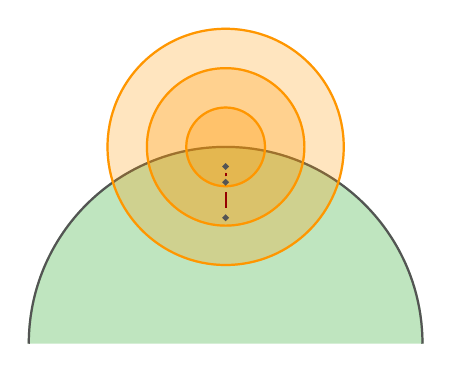
\begin{tikzpicture}[x=0.50cm,y=0.50cm]
  % colors
  \definecolor{kGreen}{rgb}{0.0,0.59,0.0}
  \definecolor{kOrange}{rgb}{1.0,0.59,0.0}
  \definecolor{kGrey}{rgb}{0.33,0.33,0.33}
  \definecolor{kRed}{rgb}{0.59,0.0,0.0}
  % shape
  \node (px) at (5,5) {};
  \draw[draw,thick,fill,color=kGreen,nearly transparent] (0,0) arc (180:0:5);
  \draw[draw,thick,color=kGrey] (0,0) arc (180:0:5);
  % balls
  \draw[draw,thick,fill,color=kOrange,nearly transparent] (px) circle (3);
  \draw[draw,thick,color=kOrange] (px) circle (3);
  \draw[draw,thick,fill,color=kOrange,nearly transparent] (px) circle (2);
  \draw[draw,thick,color=kOrange] (px) circle (2);
  \draw[draw,thick,fill,color=kOrange,nearly transparent] (px) circle (1);
  \draw[draw,thick,color=kOrange] (px) circle (1);
  % barycenters
  \node (b1) at (5,4.5) {};
  \node (b2) at (5,4.1) {};
  \node (b3) at (5,3.2) {};
  \draw[draw,thick,color=kRed, fill] (b1) -- (b2);
  \draw[draw,thick,color=kRed, fill] (b2) -- (b3);
  \draw[draw,thick,color=kGrey,fill] (b1) circle (0.05);
  \draw[draw,thick,color=kGrey,fill] (b2) circle (0.05);
  \draw[draw,thick,color=kGrey,fill] (b3) circle (0.05);
\end{tikzpicture}
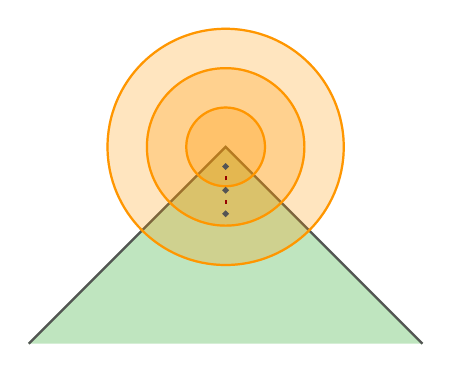
\begin{tikzpicture}[x=0.50cm,y=0.50cm]
  % colors
  \definecolor{kGreen}{rgb}{0.0,0.59,0.0}
  \definecolor{kOrange}{rgb}{1.0,0.59,0.0}
  \definecolor{kGrey}{rgb}{0.33,0.33,0.33}
  \definecolor{kRed}{rgb}{0.59,0.0,0.0}
  % shape
  \node (px) at (5,5) {};
  \draw[draw,thick,fill,color=kGreen,nearly transparent] (0,0) -- (5,5) -- (10,0);
  \draw[draw,thick,color=kGrey] (0,0) -- (5,5) -- (10,0);
  % balls
  \draw[draw,thick,fill,color=kOrange,nearly transparent] (px) circle (3);
  \draw[draw,thick,color=kOrange] (px) circle (3);
  \draw[draw,thick,fill,color=kOrange,nearly transparent] (px) circle (2);
  \draw[draw,thick,color=kOrange] (px) circle (2);
  \draw[draw,thick,fill,color=kOrange,nearly transparent] (px) circle (1);
  \draw[draw,thick,color=kOrange] (px) circle (1);
  % barycenters
  \node (b1) at (5,4.5) {};
  \node (b2) at (5,3.9) {};
  \node (b3) at (5,3.3) {};
  \draw[draw,thick,color=kRed, fill] (b1) -- (b2);
  \draw[draw,thick,color=kRed, fill] (b2) -- (b3);
  \draw[draw,thick,color=kGrey,fill] (b1) circle (0.05);
  \draw[draw,thick,color=kGrey,fill] (b2) circle (0.05);
  \draw[draw,thick,color=kGrey,fill] (b3) circle (0.05);
\end{tikzpicture}

  \end{center}
  \caption[Analyse de la variation de longueur du barycentre.]
  %
  {Analyse de la variation de la distance du barycentre $|n_R|$ sur une surface
  lisse (\emph{à gauche}) et sur une singularité (\emph{à droite}). La longueur
  croît de façon quadratique sur la surface lisse et linéairement sur la
  singularité.\label{fig:moments-explained}}
  %
\end{figure}

Ils définissent alors une analyse en espace d'échelle de $|n_R|$ (la distance de
$\vx$ au barycentre $\vb$) comme fonction du rayon du voisinage $R$ (voir
\RefFigure{fig:moments-explained}). Ils démontrent alors que cette longueur
croît de façon quadratique sur des surfaces lisses lorsque le voisinage
augmente, tandis que la longueur croît linéairement sur des singularités.
Cependant, ils n'utilisent pas cette propriété dans leur méthode de
classification et ne l'évaluent pas expérimentalement, probablement à cause de
la difficulté à distinguer les deux comportements (linéaire et quadratique)
comme le montre la \RefFigure{fig:moment-multiscale}.

\begin{figure}[ht]{
    \begin{center}
    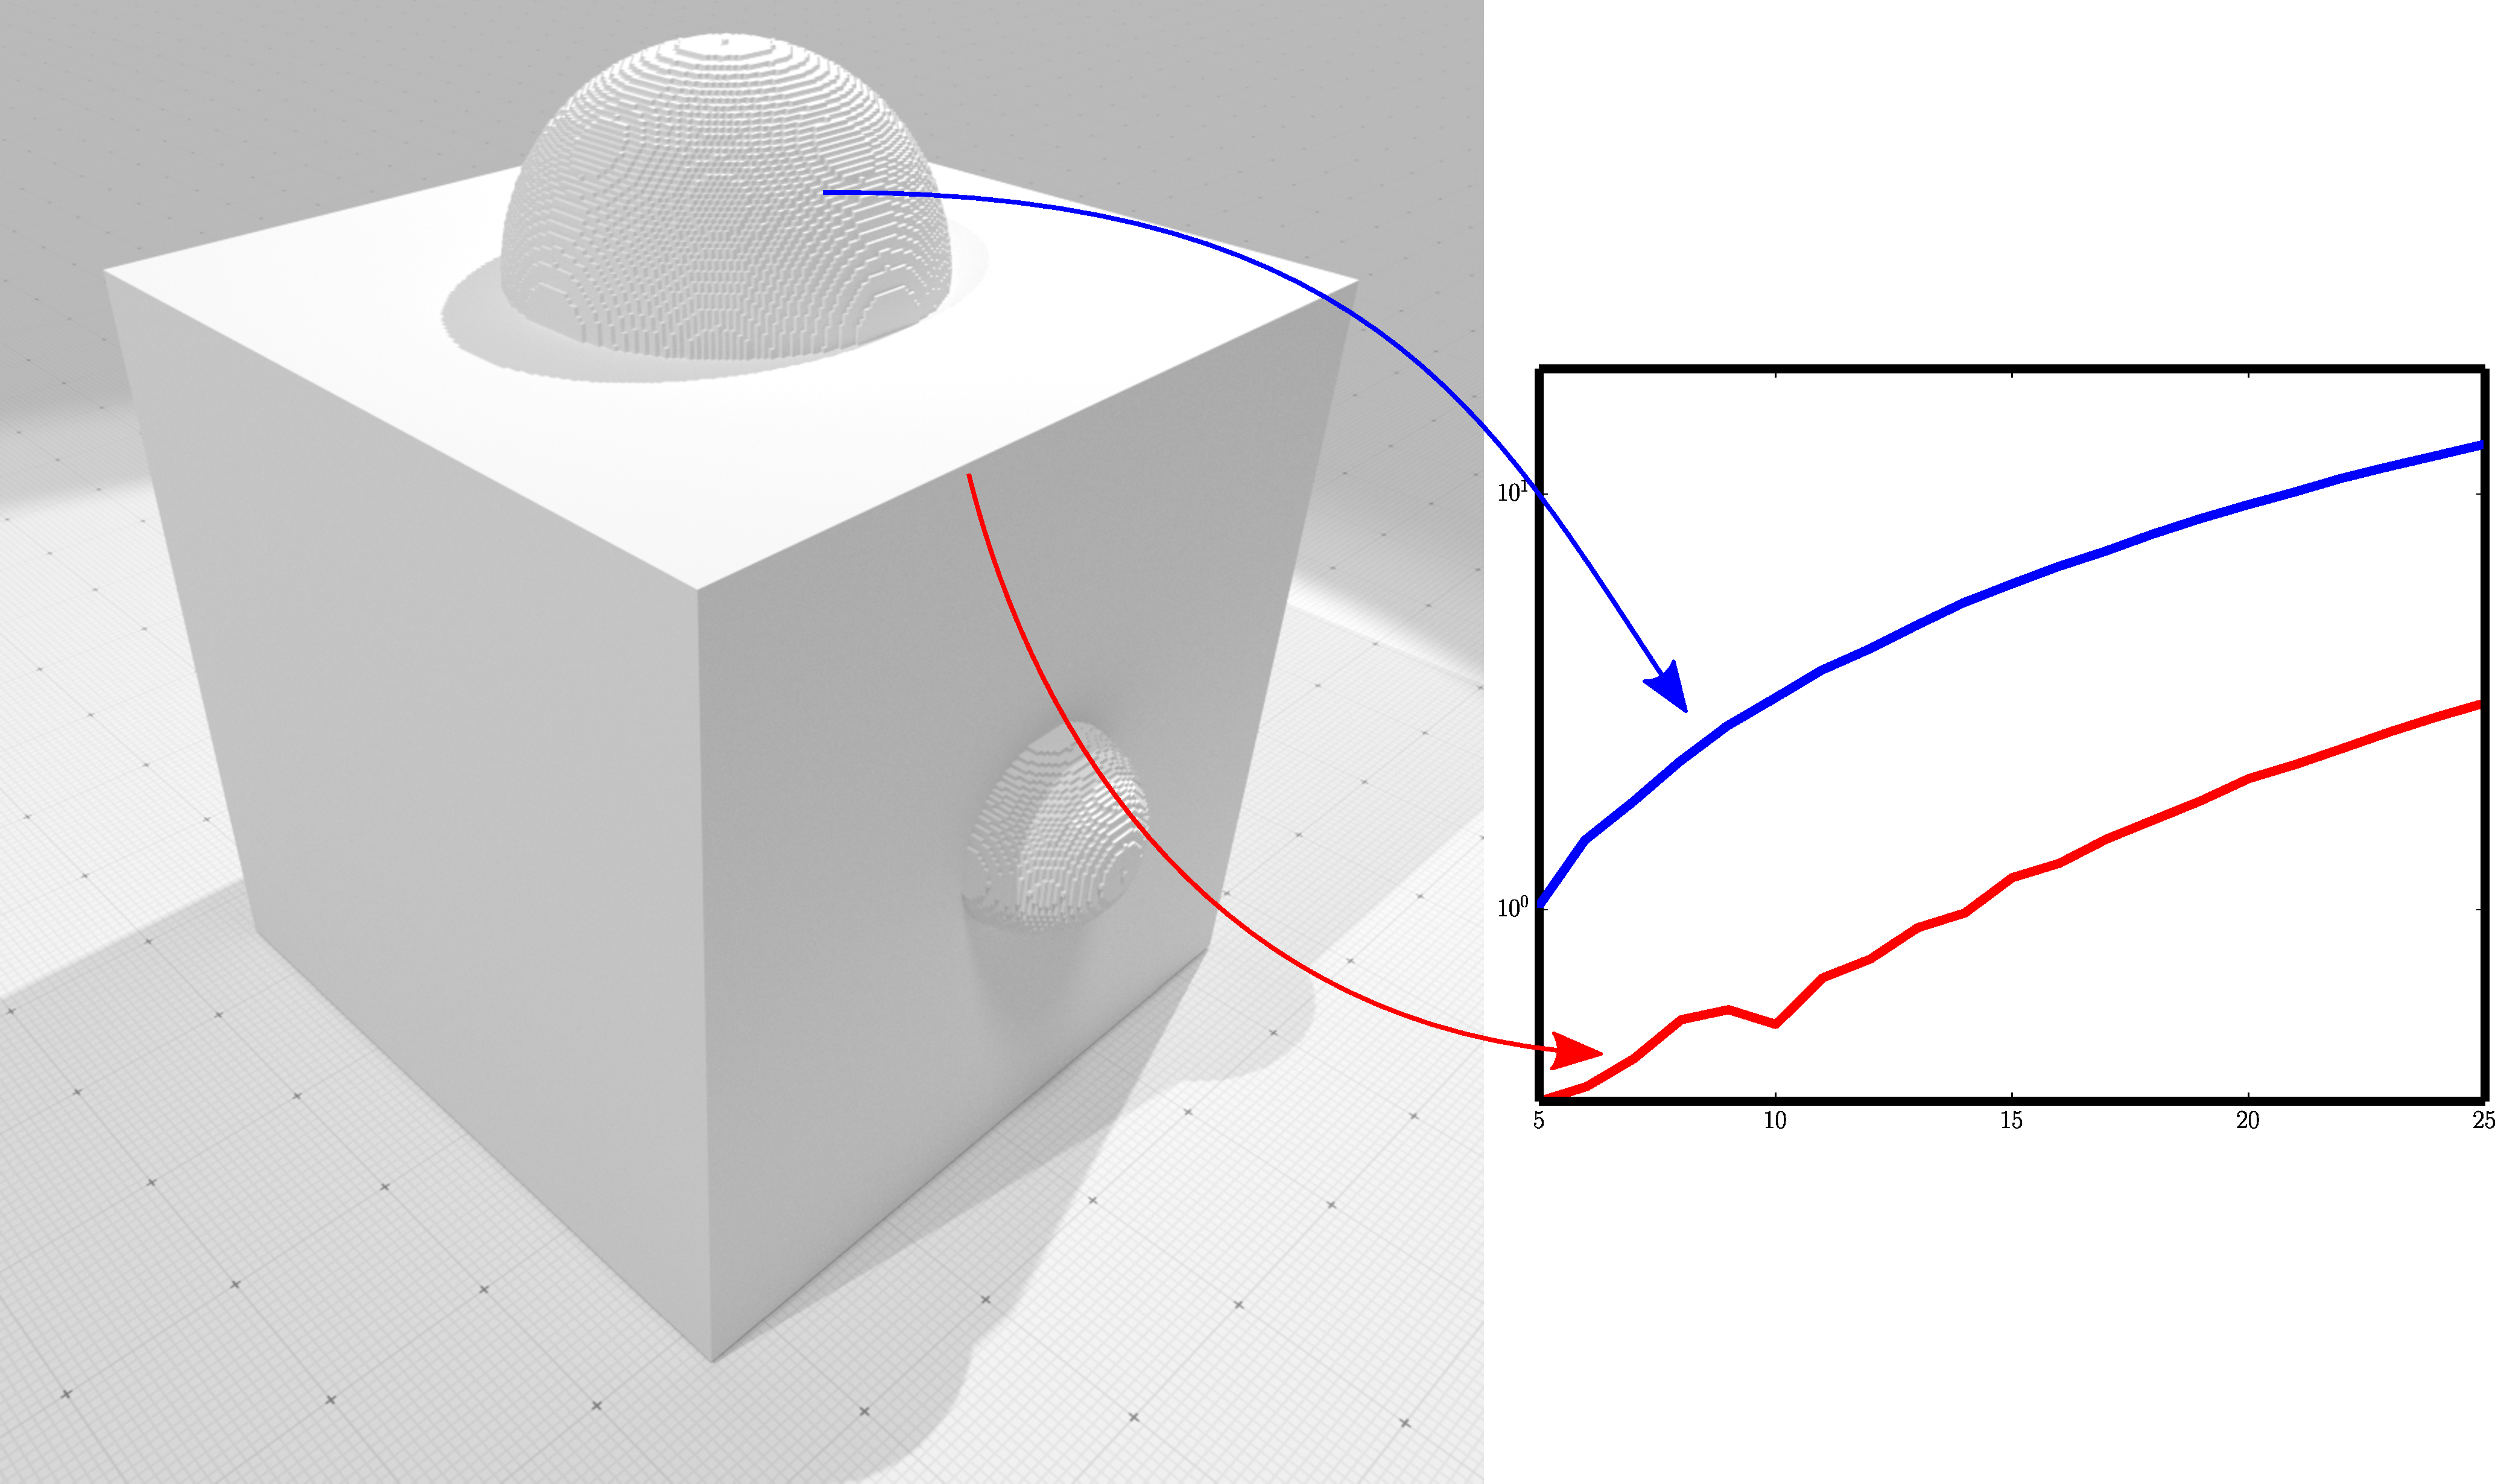
\includegraphics[height=6.8cm]{figures/CubeSpherePlotMoment_SS}
    \end{center}}
    \caption[Évolution de $n_R$ en fonction de la taille du voisinage $R$]{Évolution de $n_R$ en fonction de la taille du voisinage $R$.
      \label{fig:moment-multiscale}}
\end{figure}

Ils proposent alors deux méthodes\footnote{Notées $\mathcal{C}_{\epsilon}^{0}$
et $\mathcal{C}_{\epsilon}^{0,1}$ dans leur papier, $\epsilon \EqDef R$.} à taille de
voisinage fixe qui produisent un score de lissage :
%
\begin{itemize}
%
  \item Le premier est basé sur la longueur $|n_R|$ pour une taille donnée de
  voisinage :
  %
  \begin{equation}
    \mathcal{C}_{R}^{1} \EqDef \frac{1}{\alpha + \beta(|n_R|/R)^2} \,.
    \label{eq:moment-C0}
  \end{equation}
%
  \item Le second est basé sur la longueur $|n_R|$, la plus petite des valeurs
  propres $\lambda_{min}$ et la plus grande des valeurs propres $\lambda_{max}$
  de la matrice de covariance de $\Ball{R}{\vx} \cap \dS$ :
  %
  \begin{equation}
    \mathcal{C}_{R}^{1,2} \EqDef \frac{1}{\alpha + \beta
    \left( \frac{|n_R|~\lambda_{min}}{R~\lambda_{max}} \right)^2} \,.
    \label{eq:moment-C1}
  \end{equation}
%
\end{itemize}
%
$\alpha$ et $\beta$ sont deux paramètres (positifs), laissées à la discrétion de
l'utilisateur, pour lisser le score de zones caractéristiques et donc contrôler
la précision du calcul par rapport à la robustesse au bruit. Le second
estimateur, que nous utiliserons dans les expériences, produit des résultats
légèrement meilleurs sur des données bruitées grâce au renforcement des valeurs
propres de la matrice de covariance, liées à la normale et à la plus forte des
courbures principales.
%
%\missingfigure{Moment : Donner des résultats avec $C^0$}

\begin{figure}[hbt]
  \centering
  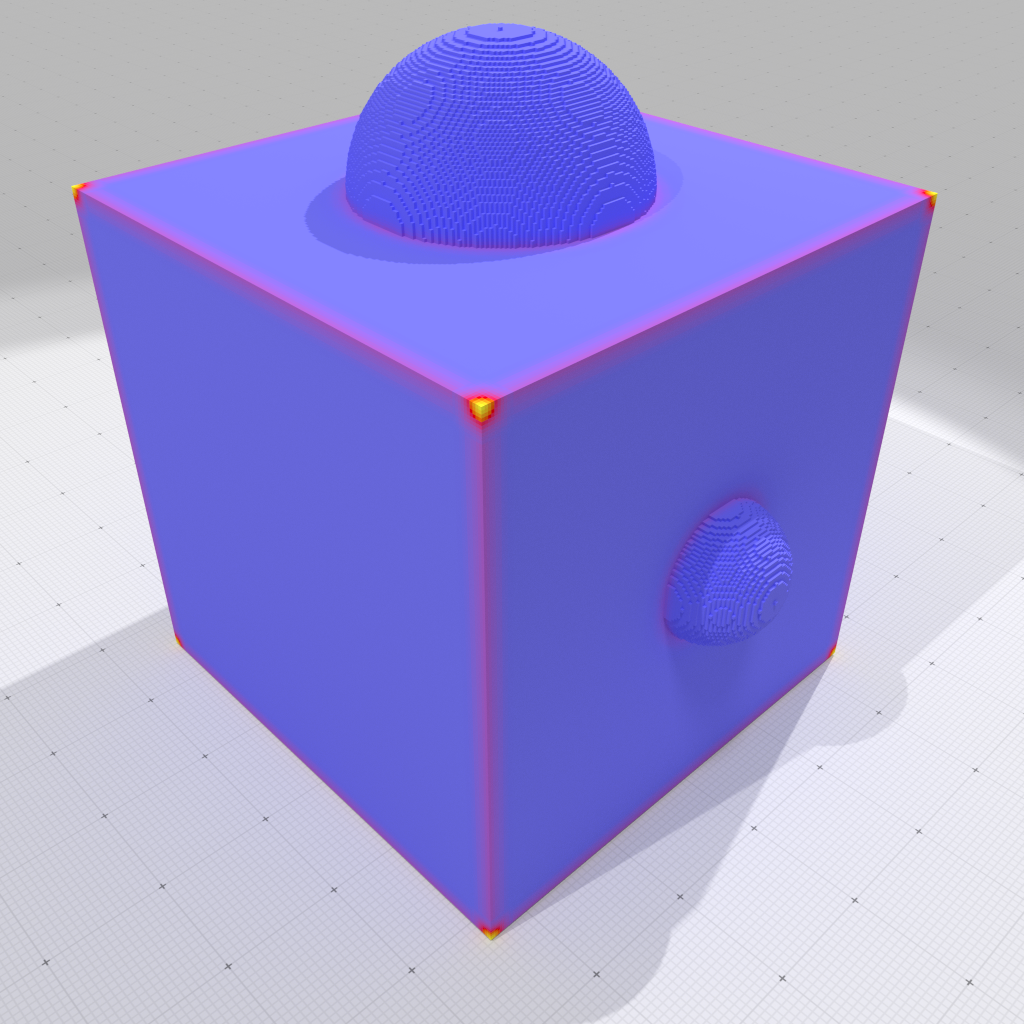
\includegraphics[height=6.8cm]{images/Feature/CubeSphere_Moments_r_10_c1}
  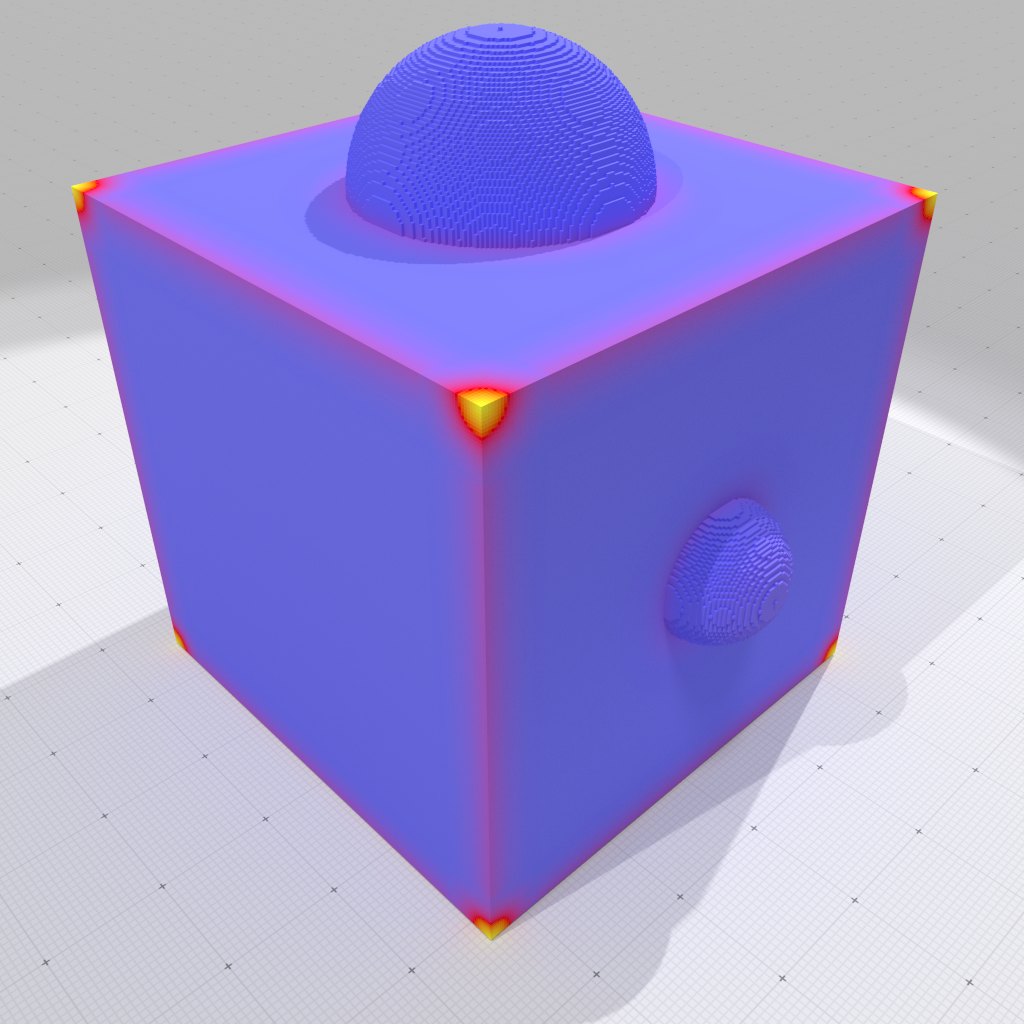
\includegraphics[height=6.8cm]{images/Feature/CubeSphere_Moments_r_22_c1}
  \caption[Résultat de l'\RefEquation{eq:moment-C1}]{Résultat de l'\RefEquation{eq:moment-C1} avec comme paramètres $\alpha = 1$, $\beta = 50$ pour deux tailles de voisinage $R = 10$ et $R = 22$.}\label{fig:moment-C1}
\end{figure}

Il y a alors trois paramètres à choisir : $\alpha$, $\beta$, ainsi que la
taille du voisinage, rendant la détection compliquée sans analyse au préalable
de la forme d'entrée. Le \RefSection{sec:applications:feature:comparison} compare le résultat de l'\RefEquation{eq:moment-C1} avec deux rayons différents.
%
\paragraph{Mesure de covariance des cellules de Voronoï}
%
Nous avons parlé de la mesure de covariance des cellules de Voronoï de
\cauthors{Mérigot}{Merigot2011} (basée sur les travaux de
\cauthors{Alliez}{Alliez2007}) dans l'état de l'art du
\RefChapitre{sec:estimators}. Pour résumer, chaque point $\vp$ est associé à une
\emph{mesure de covariance des cellules de Voronoï} $\mathcal{V}_{K,R}$ (\VCMM ---
\VCM ---) dont ils peuvent extraire des informations sur la géométrie
sous-jacente.


% Il s'agit en fait de calculer un matrice de
% covariance ($cov$) sur des cellules de Voronoï ($Vor_K$) des points du bord de
% l'objet :
% %
% \begin{equation}
%     cov(K,\vp) \EqDef \int_K (\vx - \vp)(\vx - \vp)^T d\vx .
% \end{equation}
%
%
%
% Afin d'avoir une information plus locale de la variation de la forme, ils se
% limitent à un voisinage de rayon $R$ :
% %
% \begin{equation}
%   \mathcal{V}_{K,R}(\{\vp\}) \EqDef cov(Vor_K(\vp) \cap \Ball{R}{\vp}, \vp) .
% \end{equation}
% %
% Enfin, afin d'être plus résistant au bruit de Hausdorff, ils utilisent une
% version convoluée de \VCM grâce à une fonction indicatrice $\chi_r$
% (ayant pour paramètre un rayon $r$) :
% %
% \begin{equation}
%   \mathcal{V}_{K,R} \ast \chi_r(\{\vp\}) \EqDef \int_{K^R} (\vx - \pi^K(\vx))(\vx - \pi^K(\vx))^T \chi(\pi^K(\vx) - \vp) d\vx .
% \end{equation}
% %
% où $\pi^K(\vx)$ est la projection de tout point $\vx$ vers le point le plus proche de
% $K$. $\chi_r$ peut être une fonction « Ball » ($\chi_r(\vp) = 1$ si $\vx$
% appartient à $\Ball{r}{\mathbf{0}}$, $0$ sinon) ou encore une fonction « Hat »
% ($\chi_r(\vp) = max(0, r - ||\vp||^2)$).
%
% \begin{figure}[ht]{
%     \begin{center}
%     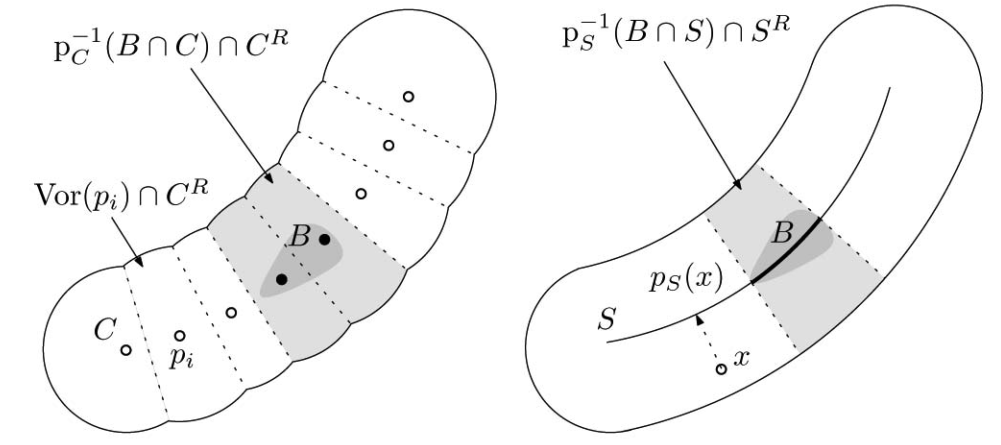
\includegraphics[height=6cm]{images/Feature/VCM_notations}
%     \end{center}}
%     \caption[Notations de \VCM.]{Notations de \VCM (Figure~5 de \cite{Merigot2011}). La figure de gauche est sur un nuage de points tandis que celle de droite est sur une forme continue. \label{fig:VCM-multiscale}}
% \end{figure}
%
%
% À noter que \cauthors{Cuel}{Cuel2014DGCI} ont défini une variante digitale du
% \VCM ($\DigShape \in \Z^3$) :
% %
% \begin{equation}
%   \hat{\mathcal{V}}_{\DigShape,h,R} \ast \chi_r(\{\vp\})) \EqDef \sum_{\vx \in \Omega_h^R} h^3 (\vx - \pi^{\DigShape}(\vx)) (\vx - \pi^{\DigShape}(\vx))^t \chi(\pi^{\DigShape}(\vx)) ,
% \end{equation}
% %
% où $\Omega_h^R$ est l'ensemble des (centres de) voxels entièrement contenus dans
% $\DigShape^R$ (la $R$-dilatation de $\DigShape$) au pas de discrétisation $h$.
% %
% Il est à noter que la convergence asymptotique de cette variante digitale de
% l'estimateur \VCM pour les normales a été prouvée (bord de la surface de classe
% $C^2$ et de reach $\rho > 0$) \cite{Cuel2014DGCI}.


L'estimateur \VCM a alors besoin de deux paramètres : le rayon de dilatation $R$
de l'ensemble d'entrée (la fonction distance est plus robuste lorsqu'elle est
loin de la surface), et le rayon de convolution $r$ qui définit quelles cellules
de Voronoï vont être intégrées pour lisser la mesure. Ces deux paramètres
permettent également de limiter l'impact du bruit sur la surface tout en
préservant les informations géométriques. Un score de point caractéristique
$r(\vp)$ est alors calculé à l'aide d'un ratio des valeurs propres de la
convolution du \VCM $\mathcal{V}_{K,R} \ast \chi_r(\{\vp\})$ pour chaque point
$\vp$ :
%
\begin{equation}
  r(\vp) \EqDef \frac{\lambda_2(\vp)}{\lambda_0(\vp) + \lambda_1(\vp) + \lambda_2(\vp)} \,.
  \label{eq:VCM-ratio-eigenvalues}
\end{equation}
%
Le point est alors considéré comme une singularité si son ratio est supérieur à
un paramètre de seuillage $T$ donné par l'utilisateur.

\begin{figure}[ht]
  \centering
  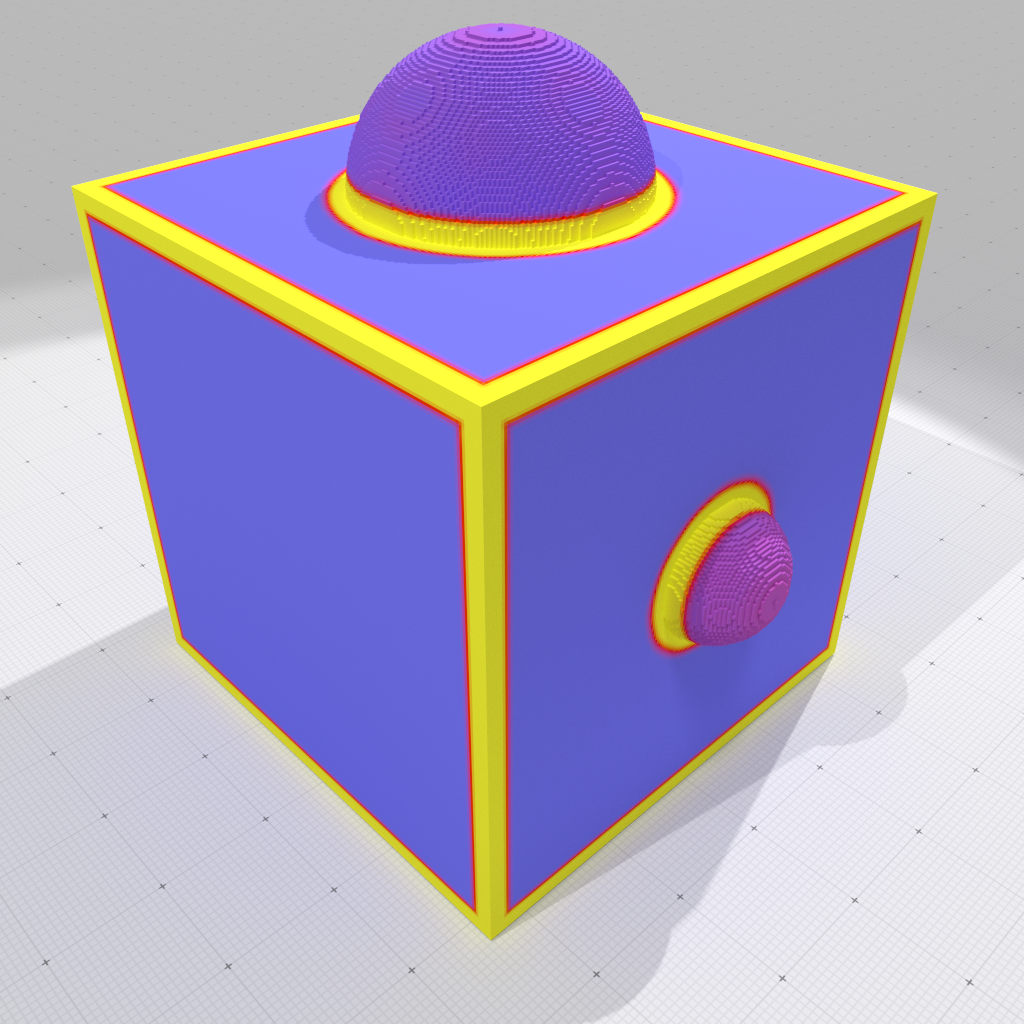
\includegraphics[height=6.8cm]{images/Feature/CubeSphere_VCM_r_10}
  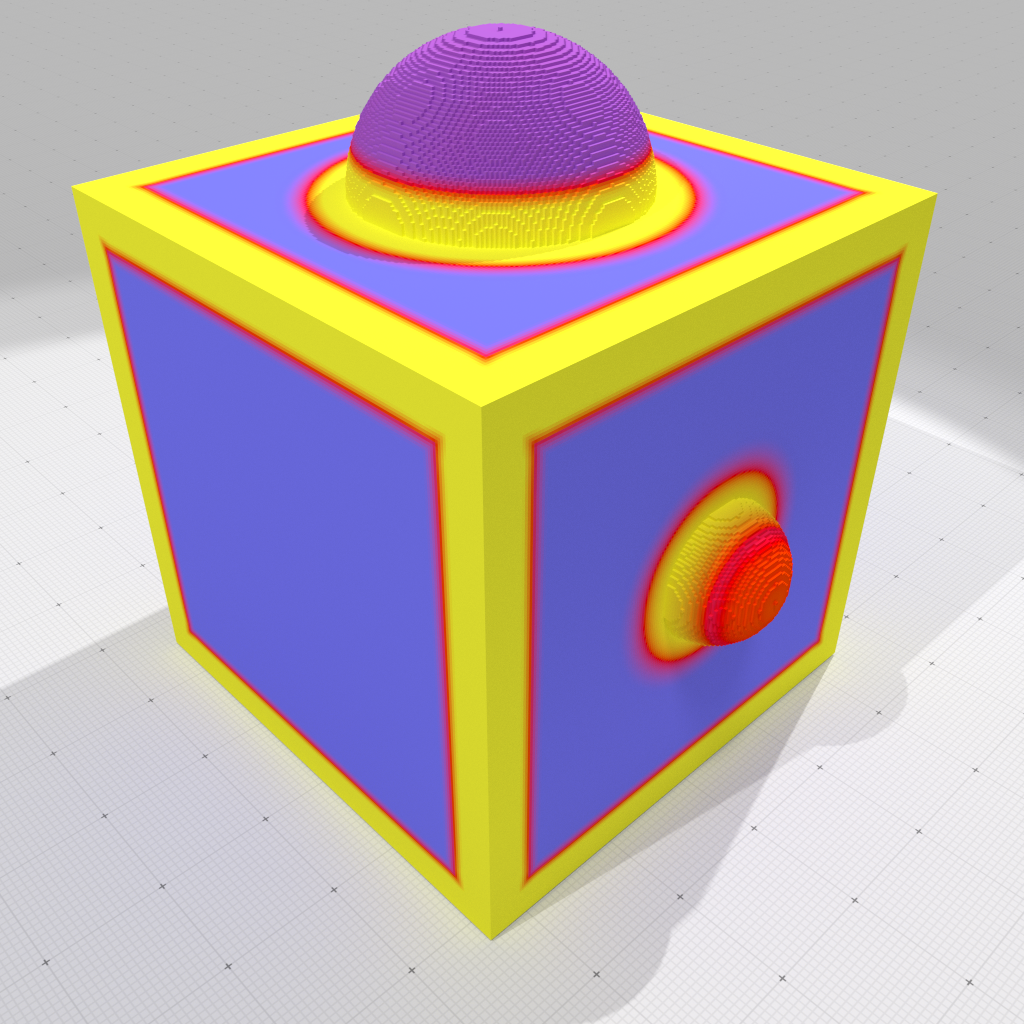
\includegraphics[height=6.8cm]{images/Feature/CubeSphere_VCM_r_22}
  %
  \caption[Résultat de l'\RefEquation{eq:VCM-ratio-eigenvalues}]{Résultat de
  l'\RefEquation{eq:VCM-ratio-eigenvalues} avec comme paramètres $T = 0.2$, $R_1 =
  10$, $r_1 = 10$ (\emph{à gauche}) et $R_2 = 22$, $r_2 = 22$ (\emph{à
  droite}).}\label{fig:VCM-cubesphere}
  %
\end{figure}

\paragraph{Vote de tenseur}
%
%\todoJeremy{more citations}
%
Dans un esprit similaire aux méthodes précédentes, certains auteurs
\cite{Park2012} ont proposé une stratégie de vote de tenseur (\anglais{Tensor
Voting}) sur des morceaux surfaciques. Ce dernier, défini par
\cauthors{Medioni}{Medioni2000-2} est l'intégration du tenseur des points d'un
voisinage, contenant des informations de la surface sous-jacente. Ils utilisent
alors un comportement en espace d'échelle du vote du tenseur lorsque la taille du
voisinage augmente afin d'extraire les singularités sur des nuages de points.
Cependant, ces méthodes sont très sensibles et ne produisent pas de résultats
suffisamment robustes sur des données digitales.


Plus concrètement, pour un voisinage donné \footnote{Des contraintes de
connectivité et d'uniformité entrent en jeu, mais sont satisfaites sur une grille
régulière digitale.}, \cauthors{Park}{Park2012} accumulent dans une matrice les
tenseurs :
%
\begin{equation}
  T_i = \sum\limits_{j \in N(i)} \left(\mathcal{I}_3 - \frac{\overrightarrow{v}_j\overrightarrow{v}_j^T}{||\overrightarrow{v}_j\overrightarrow{v}_j^T||} \right) \,,
\end{equation}
%
avec $\overrightarrow{v}_j = \overrightarrow{x}_j - \overrightarrow{x}_i$.

\begin{figure}[ht]{
    \begin{center}
    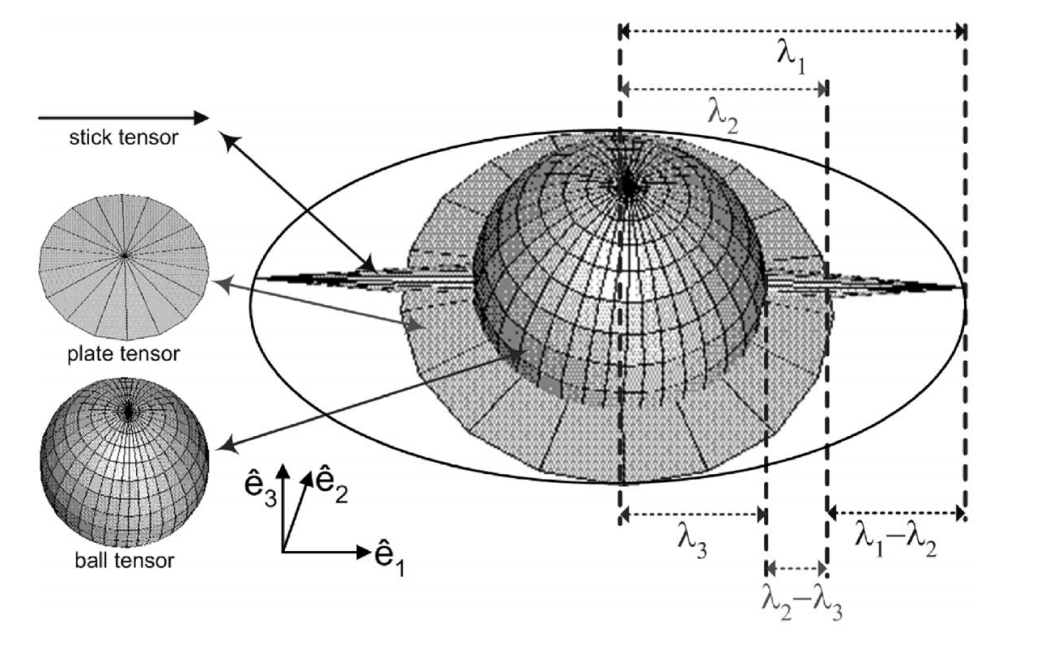
\includegraphics[height=7cm]{images/Feature/Tensor_voting_notations}
    \end{center}}
    \caption{Les trois différents type de tenseur de la théorie du vote de tenseur \cite{Medioni2000-2}. Nous utiliserons ici uniquement le tenseur de boule.
      \label{fig:TV-multiscale}}
\end{figure}

Avec un ratio sur les valeurs propres de cette matrice, \nauthors{Park} veulent
obtenir un poids $\omega_i$ déterminant si le point est caractéristique :
%
\begin{equation}
  \omega_i = \frac{\lambda_2 + \lambda_3}{\lambda_1},
\end{equation}
%
et ainsi classifier la surface en deux catégories : \Feature (\cad dans le cas
présent une singularité) et \NonFeature.


L'analyse en espace d'échelle intervient au niveau du seuillage avec les poids
calculés à partir des matrices. Deux bornes sont alors définies par
l'utilisateur : $\omega^-$ et $\omega^+$, celles-ci correspondent au seuil
inférieur et supérieur de la variation de $\omega_i$ en fonction du rayon. En
effet, sur des zones à forte courbure, le poids sera plus élevé que sur des
zones à courbure nulle. Bien que le poids soit stable quelle que soit l'échelle sur
ces zones, l'analyse à plusieurs rayons permet de capturer des zones de
saillance qui auraient pu ne pas être considérées à une échelle donnée; c'est le
cas d'une zone lisse ou proche d'une singularité par exemple où $\omega_i$ croîtra
(\RefFigure{fig:tensor-weight}).

\begin{figure}[ht]{
    \begin{center}
    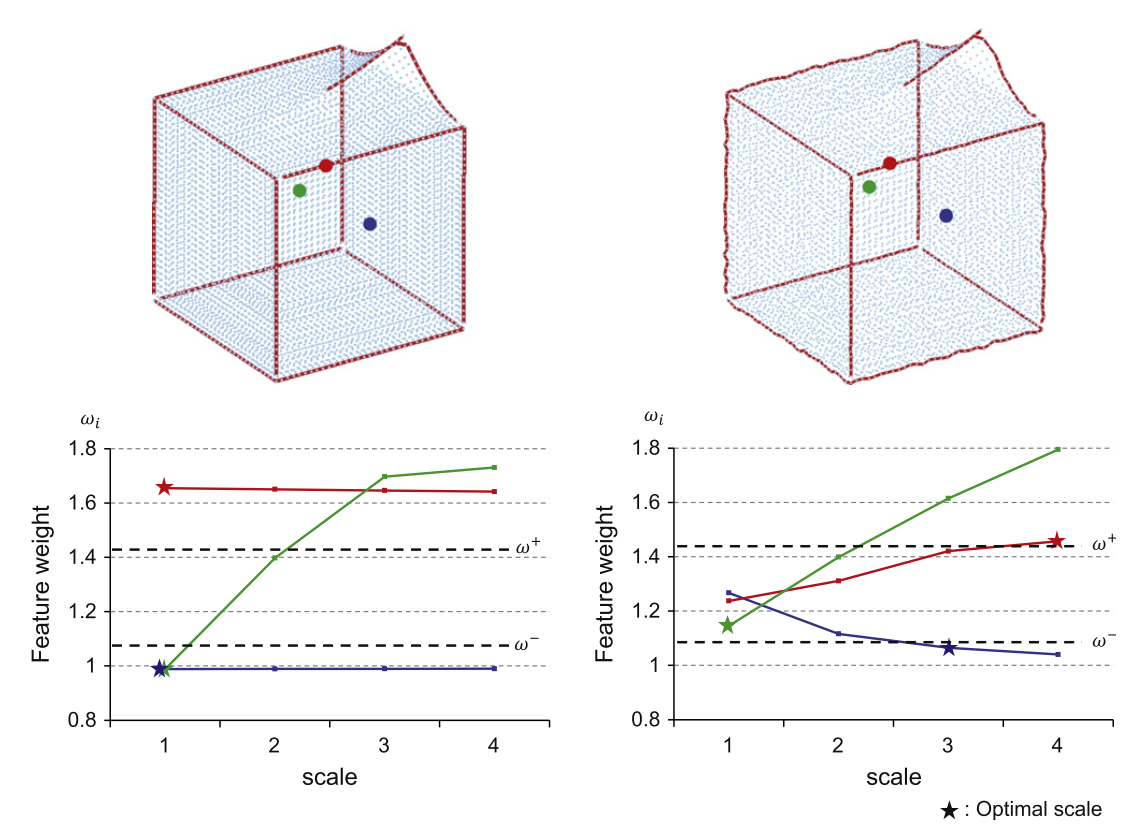
\includegraphics[height=10cm]{images/Feature/Tensor_weight}
    \end{center}}
    \caption[Variation du poids $\omega_i$.]{Variation du poids $\omega_i$ (Figure~6 de \cite{Park2012}).
      \label{fig:tensor-weight}}
\end{figure}

Ainsi, pour tous les rayons, si le poids devient plus grand que $\omega^+$, le
point sera labellisé comme \Feature (en rouge sur
\RefFigure{fig:tensor-cubesphere}); si le poids devient plus petit que
$\omega^-$ alors le point sera labellisé comme \NonFeature (en vert); si le
poids est entre $\omega^-$ et $\omega^+$, nous allons regarder la variation du
poids : si le poids est supérieure à $\tau$ fois le poids au rayon précédent,
nous gardons le précédent poids. Cette dernière condition permet d'éliminer les
résultats erronés dus au bruit par exemple, introduisant une forte
variation. Ces points seront traités plus tard. Pour tous les autres points
(donc ceux qui ne sont pas labellisés \Feature, \NonFeature ou avec une forte
variation de poids), nous allons effectuer la même vérification à l'échelle
supérieure. Enfin, pour tous les points restant non labellisés, un regroupement
(\emph{clustering}) sera fait afin de traiter les regroupements de moins de
$n_{min}$ points\footnote{Dans leur article, les auteurs choisissent
arbitrairement $n_{min}=10$, mais ajoutent que cette valeur peut varier en
fonction de la densité de points.} comme \NonFeature, les autres regroupements
comme \Feature.

\begin{figure}[ht]{
  \begin{center}
    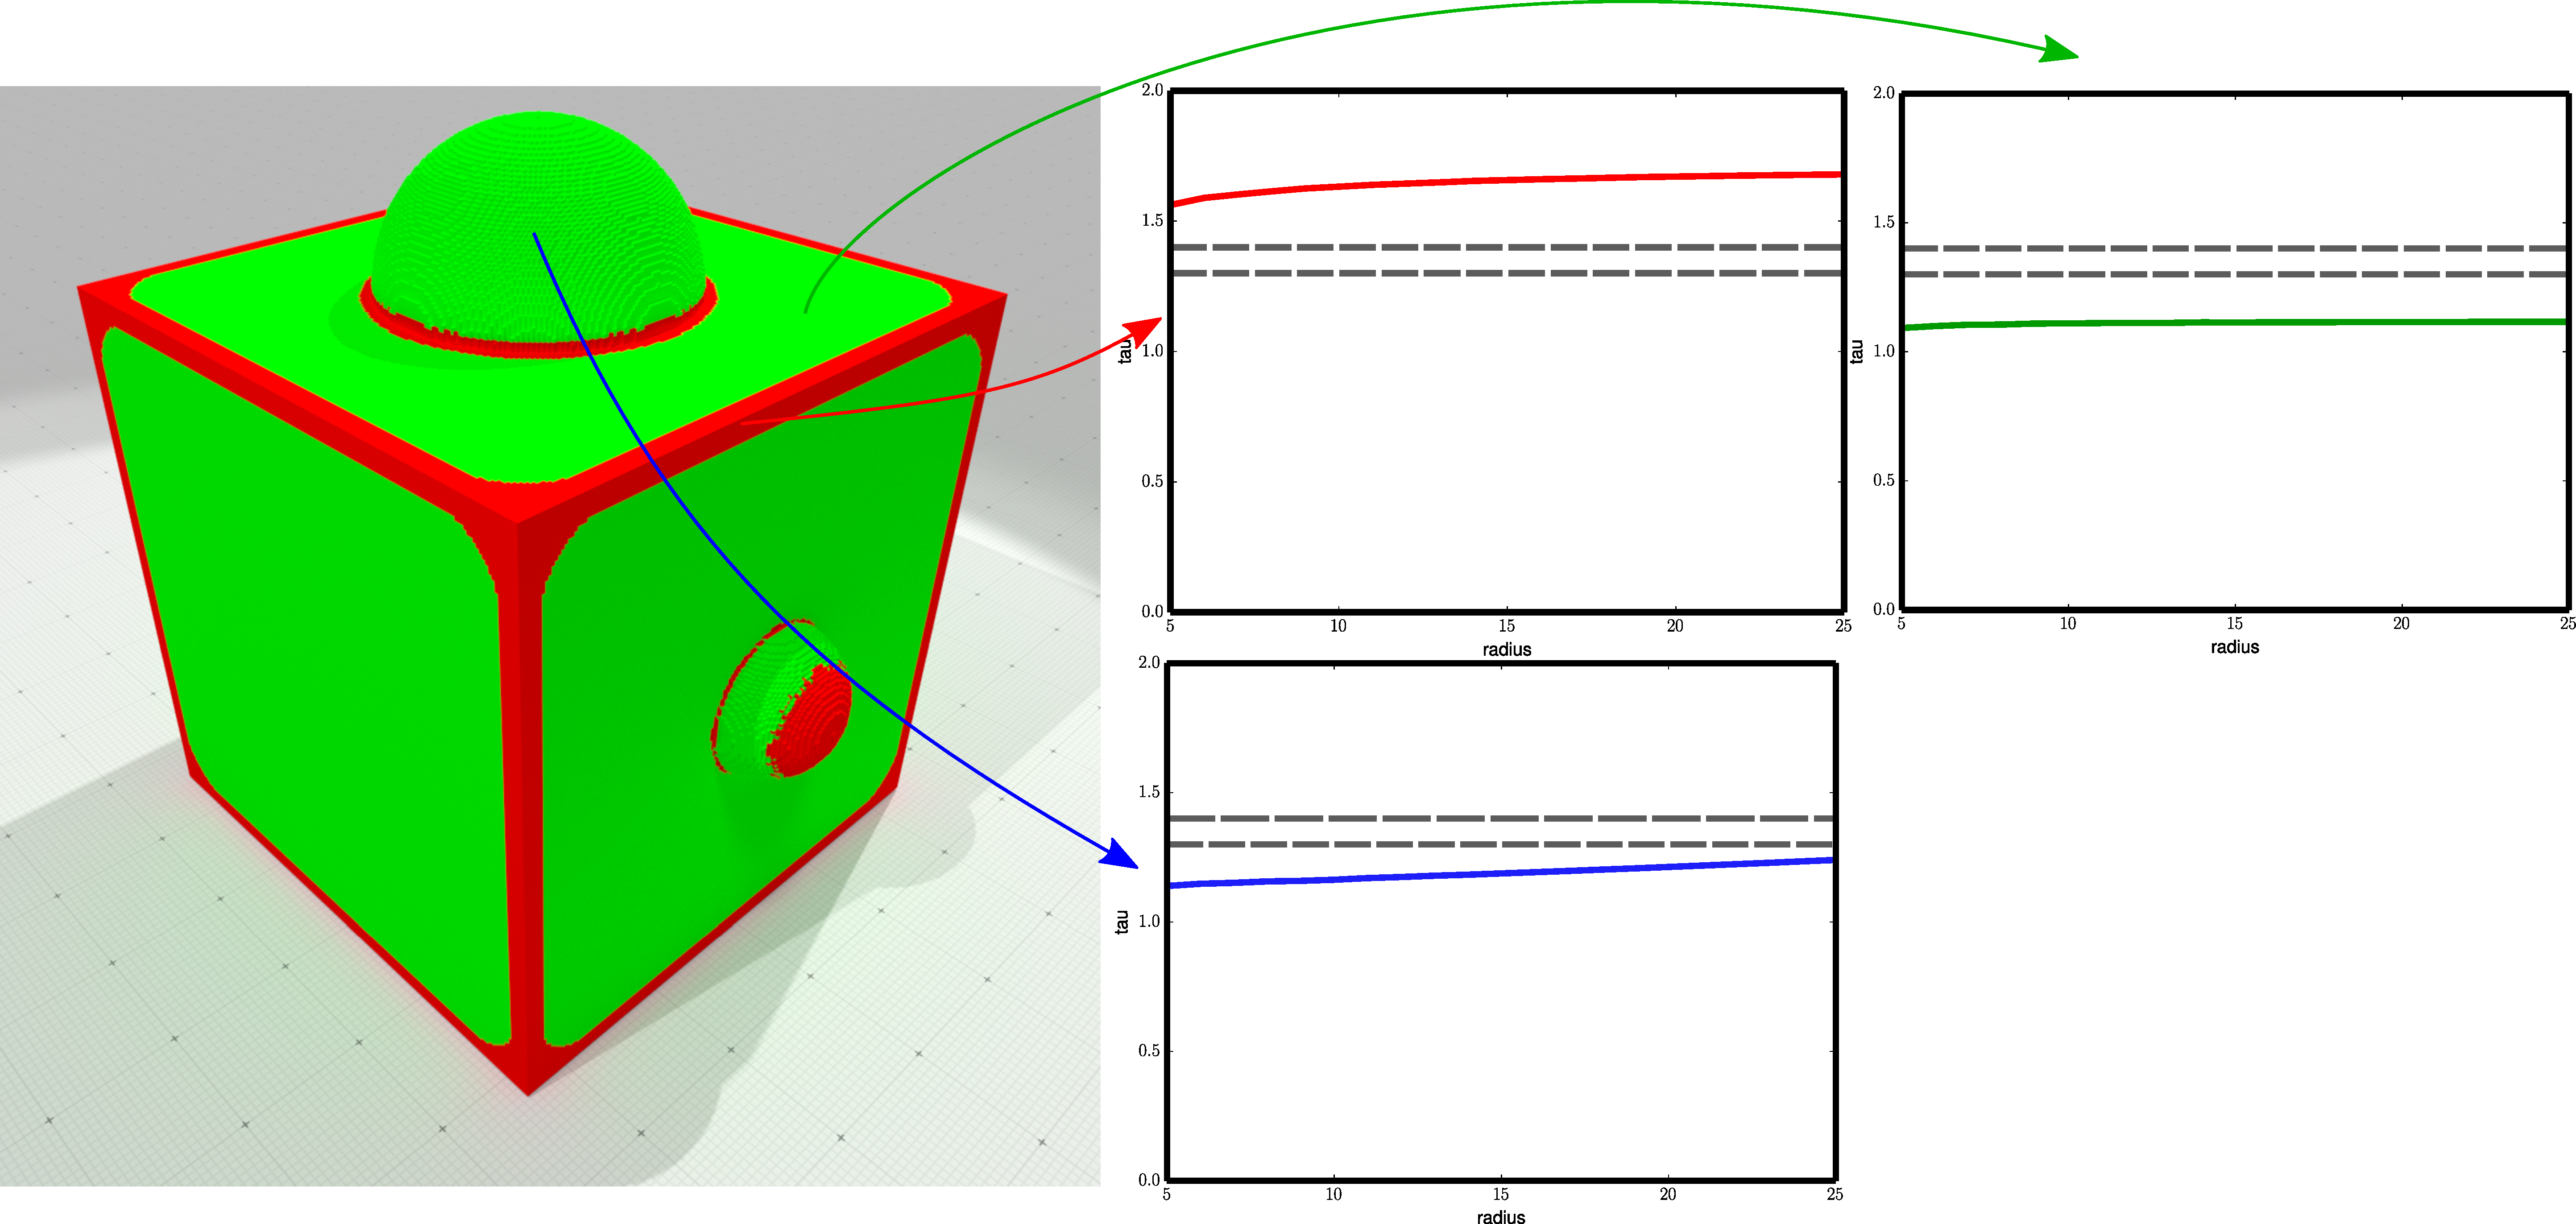
\includegraphics[height=6.6cm]{figures/CubeSpherePlotTensor}
  \end{center}}
    %
    \caption[Variation du poids $\omega_i$.]{Variation du poids $\omega_i$ à
    trois points différents : sur une partie lisse (\emph{en bleu}), sur une
    partie à courbure nulle (\emph{en vert}) et sur une singularité (\emph{en
    rouge}). Les lignes en pointillés sur les graphes sont respectivement
    $\omega^- = 1.3$ et $\omega^+ = 1.4$.\label{fig:tensor-cubesphere}}
    %
\end{figure}


Expérimentalement, $\omega^-$ et $\omega^+$ sont très dépendants de la géométrie
de la forme à analyser, et de ce que nous voulons extraire comme « zones
caractéristiques ». Une analyse plus complète est proposée dans le
\RefSection{sec:applications:feature:comparison}.
%
\paragraph{Approximation aux moindres carrés de sphères}% \comJeremy{approximation aux moindres carrés de sphères}
\label{sec:applications:feature:growing}
%
D'autres auteurs \cite{Mellado2012} ont introduit une approche rapide d'approximation
aux moindres carrés de sphères sur un nuage de points pour créer un score de
zones caractéristiques multi-échelles. À nouveau, le paramètre d'espace d'échelle
est la taille de voisinage.


Dans leurs travaux, \cauthors{Mellado}{Mellado2012} proposent d'approximer aux
moindres carrés des sphères (\emph{least squares spherical fitting}) à la
surface de l'objet, et d'en extraire un score de \emph{feature} sur chaque
élément de la surface. Le paramètre d'espace d'échelle est la taille du
voisinage à considérer dans l'approximation. En utilisant leurs notations, pour
toutes les échelles $t$ ($t=R$ avec nos notations), ils font correspondre une
hyper-sphère algébrique. Ils notent $\tau$ comme la distance de décalage
algébrique entre le point $\vp$ et la $0$-isosurface, $\eta$ comme la normale
unité et $\kappa$ comme la courbure (signée) de l'hyper-sphère.

\begin{figure}[ht]{
    \begin{center}
    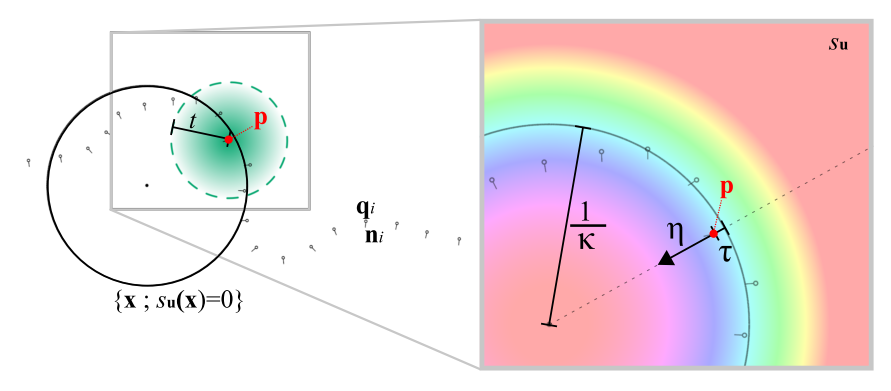
\includegraphics[height=6cm]{images/Feature/Mellado_notations}
    \end{center}}
    \caption[Notations.]{Notations (Figure~1 de \cite{Mellado2012}).
      \label{fig:mellado-notations}}
\end{figure}

Ils proposent alors de calculer la \emph{variation géométrique} au point $\vp$
définie telle que :
%
\begin{equation}
  \nu(\vp,t) \EqDef
  {\left(
    \frac{d\tau}{dt} \right)}^2
    + {\left( t\frac{d\eta}{dt}
  \right)}^2
  + {\left( t^2\frac{d\kappa}{dt} \right)}^2.
\end{equation}
%
Les auteurs laissent l'utilisateur déterminer ce qu'il considère comme un point
caractéristique en seuillant par exemple cette variation géométrique.

\begin{figure}[ht]{
    \begin{center}
    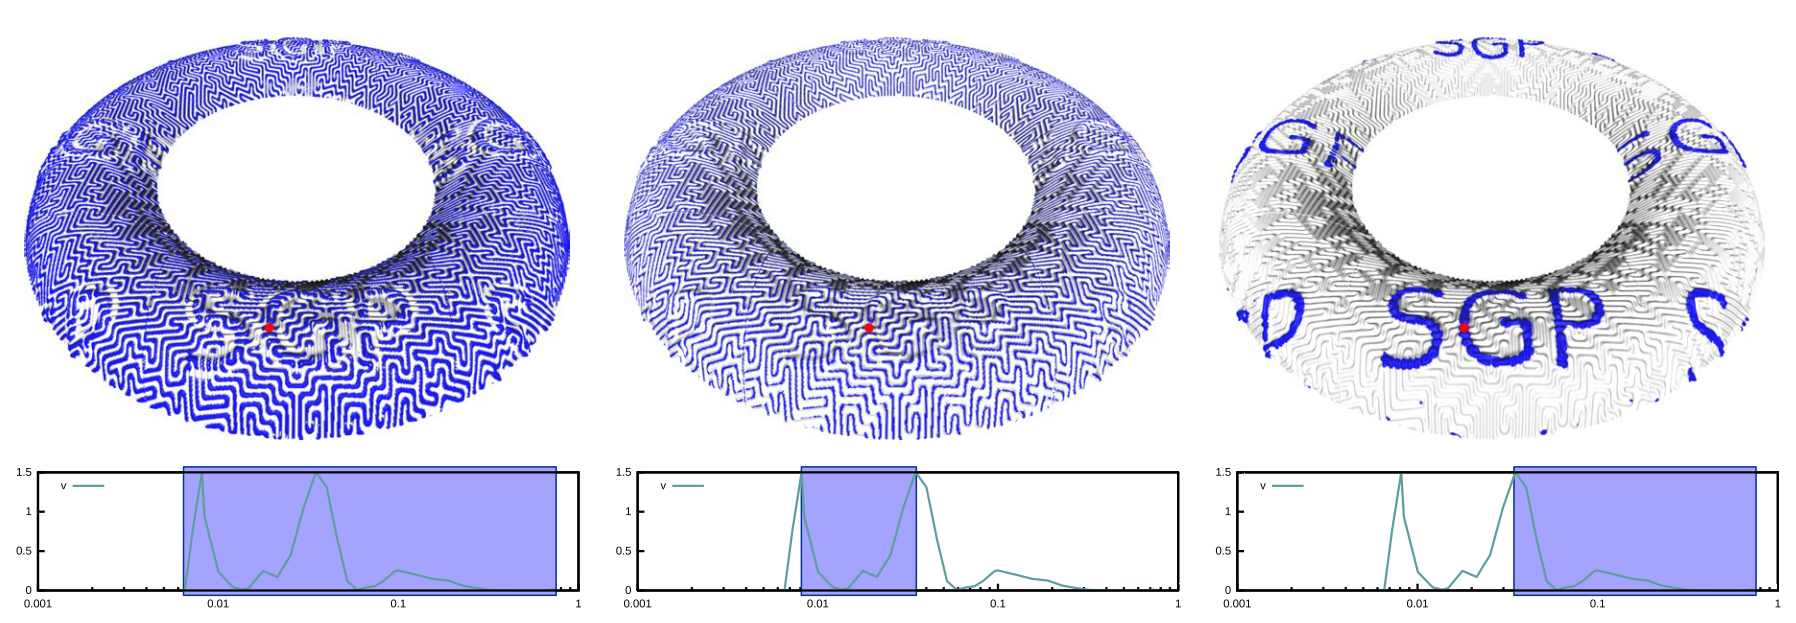
\includegraphics[width=14cm]{images/Feature/Mellado_multiscale}
    \end{center}}
    \caption[Sélection des points caractéristiques par l'utilisateur.]{Sélection des points caractéristiques par l'utilisateur en fonction de la variation géométrique $\nu$ (Figure~11 de \cite{Mellado2012}).
      \label{fig:mellado-multiscale}}
\end{figure}

Cependant, ils déterminent également une autre fonction continue d'estimation de
singularités $f$ intégrant toutes les échelles :
%
\begin{equation}
   f(\vx) \EqDef \int \tanh(\nu(\vx,t)) dt .
\end{equation}
%
Cette fonction permet de différencier les régions sans variations géométriques (en bleu sur
la \RefFigure{fig:mellado-cubesphere}) de celles qui ont de hautes variations
(en jaune)\footnote{$\tanh(\vx)$ est souvent utilisée pour renforcer les
variations \comJeremy{tout en les bornant}.}.

\begin{figure}[ht]{
  \begin{center}
    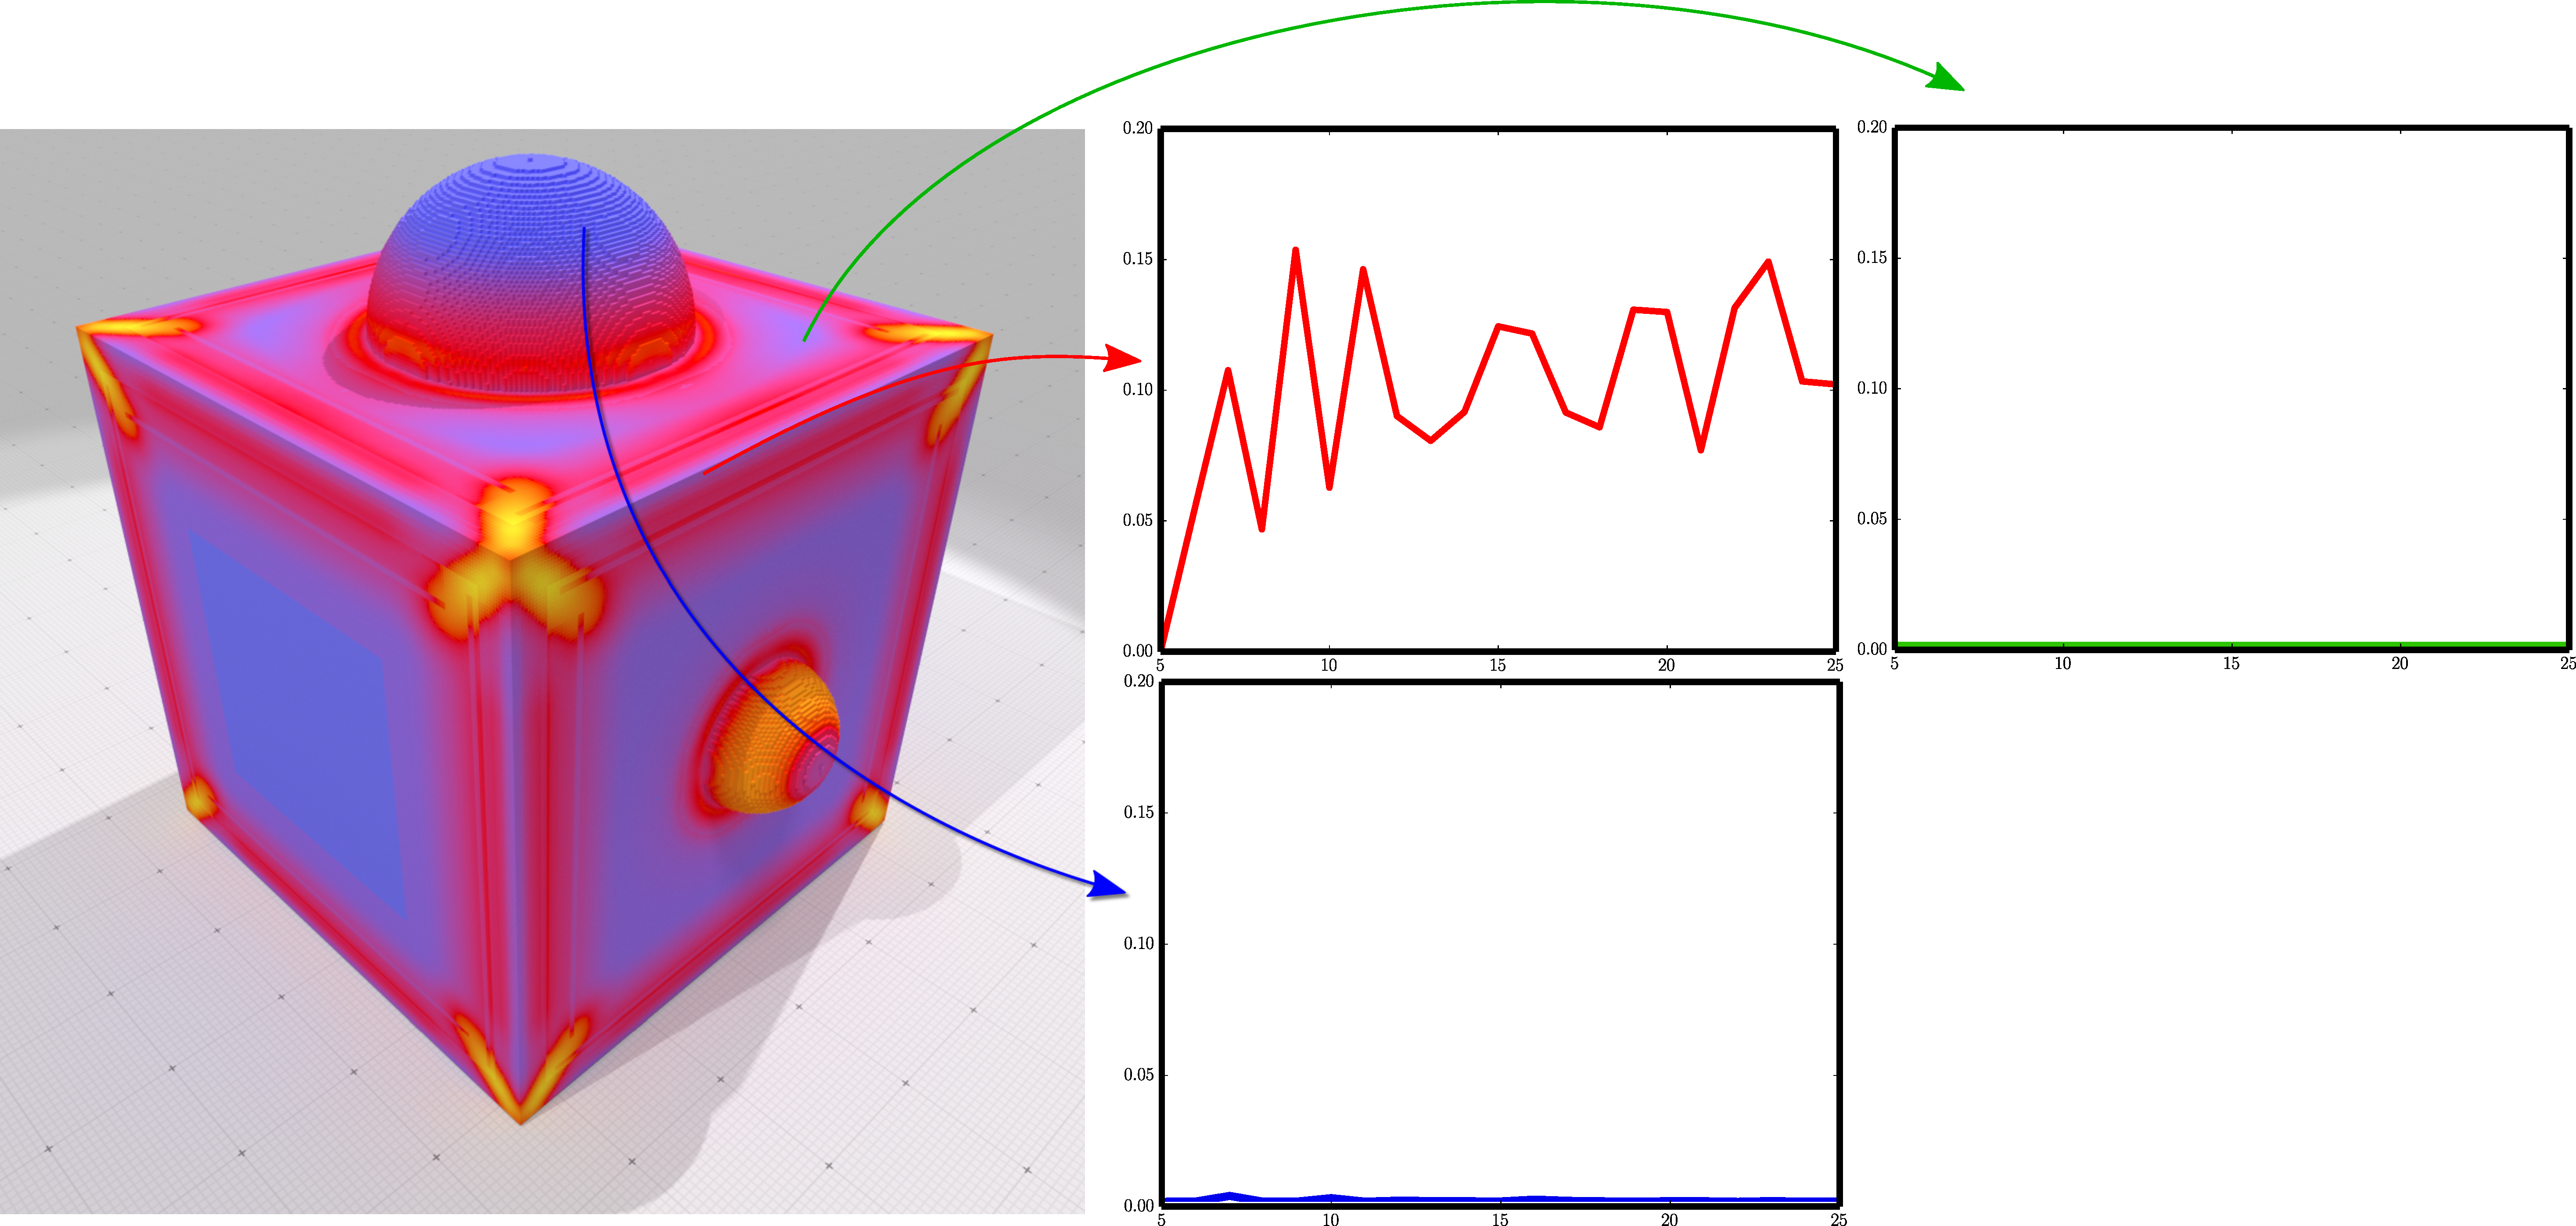
\includegraphics[height=6.8cm]{figures/CubeSpherePlotMellado}
  \end{center}}
  %
  \caption[Valeur de la fonction $f$ en tout point de la surface sur
  l'objet \CubeSphere.]{Valeur de la fonction $f$ en tout point de la surface sur
  l'objet \CubeSphere. Visualisation des valeurs de $\nu(\vx,t)$ en changeant le
  rayon $t$. \label{fig:mellado-cubesphere}}
    %
\end{figure}

Expérimentalement, cette méthode semble moins sensible au bruit, mais des
artefacts apparaissent sur les singularités (voir le
\RefSection{sec:applications:feature:comparison} pour une comparaison).


Le principal défaut de cette méthode est qu'elle ne fournit pas de quantité
exploitable directement reliée à des quantités géométriques (comme la courbure
par exemple). Expérimentalement, la quantité permet de différencier les zones
caractéristiques, mais ne repose sur aucune preuve théorique.

\subsubsection{Méthodes basées sur de l'analyse spectrale}%
\label{sec:applications:feature:spectral}

Enfin, les zones caractéristiques peuvent être extraites grâce à une analyse
spectrale sur le bord de la forme en utilisant les valeurs propres de cette matrice
laplacienne de la surface \cite{GebalBAL09,Sun2009,Song2014}. Dans ce contexte,
la saillance est caractérisée par des quantités spectrales qui sont localement
stables et distinguables de leur voisinage.
%
\paragraph{Matrice laplacienne multi-échelle}
%
\cauthors{Song}{Song2014} se sont alors penchés sur l'analyse du spectre de la
matrice laplacienne afin d'extraire des informations de saillance. La matrice laplacienne $L$ (de taille $n \times n$, $n$ étant le nombre
de sommets) est définie comme :
%
\begin{equation}
  L = W - D \,,
\end{equation}
%
où $W$ est la matrice d’adjacence à laquelle nous incorporons des informations
géométriques entre les sommets, telles que :
%
\begin{equation}
  A(i,j) =
  \begin{cases}
    1   & \text{si } p_i \text{ et } p_j \text{ sont voisins},\\
    0   & \text{sinon},\\
  \end{cases},
\end{equation}
%
\begin{equation}
  W(i,j) = \frac{1}{{||p_i - p_j||}^2}A(i,j) \,,
\end{equation}
%
et $D$ une matrice diagonale dans laquelle $D_{i,i}$ est le degré du sommet
$p_i$.


Alors, le spectre laplacien est calculé à partir des valeurs propres $\lambda_i$
(ou fréquences) de $L$ :
%
\begin{equation}
  \mathcal{H}(i) = \{ \lambda_i, 1 \le i \le n \}.
\end{equation}

\begin{figure}[ht]{
    \begin{center}
    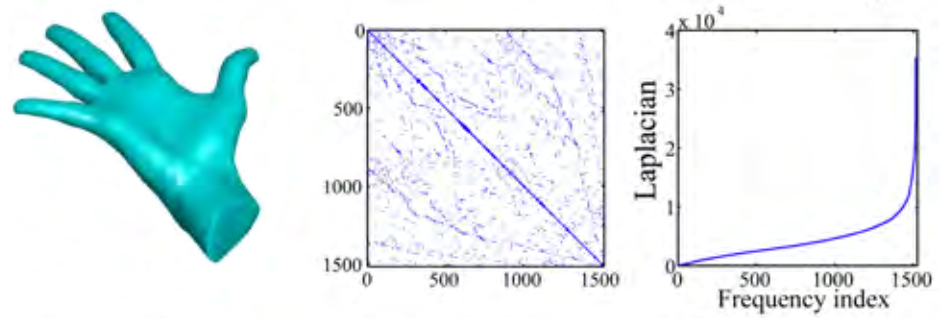
\includegraphics[width=10cm]{images/Feature/LaplacianSpectrum}
    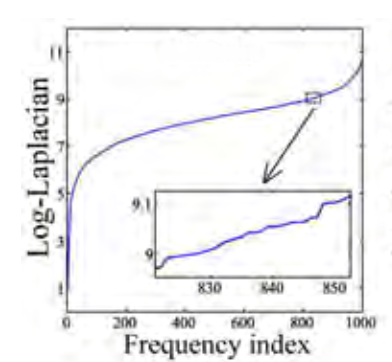
\includegraphics[width=3.5cm]{images/Feature/LaplacianSpectrumLog}
    \end{center}}
    \caption[Matrice laplacienne et son spectre.]{Matrice laplacienne $L$ et son spectre $\mathcal{H}$ et son spectre logarithmique $\mathcal{L}$ (Figures~1 et 5 de \cite{Song2014}).
      \label{fig:laplacian-spectrum}}
\end{figure}

Plus récemment, \cauthors{Hou}{Hou2007} ont utilisé le logarithme du spectre de
Fourier pour détecter les saillances visuelles d'images 2D. \nauthors{Song}
s'inspirent de cette méthode en utilisant le spectre logarithmique de la matrice
laplacienne :
%
\begin{equation}
  \mathcal{L}(i) = \log(|\mathcal{H}(i)|) \,,
\end{equation}

\begin{figure}[ht]{
    \begin{center}
    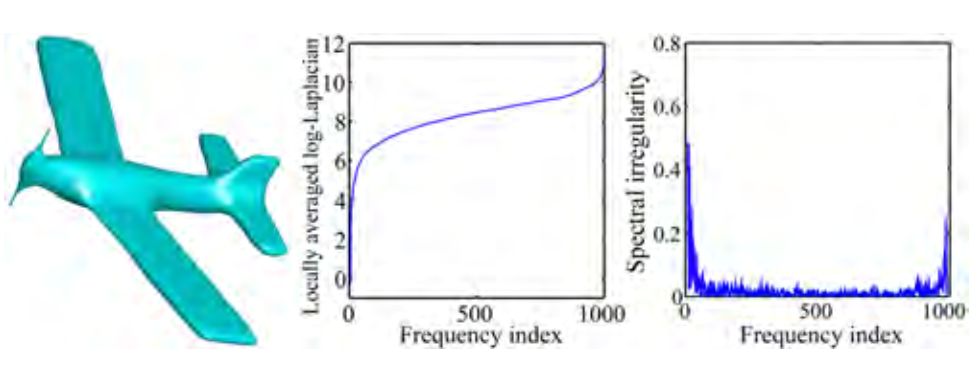
\includegraphics[width=14cm]{images/Feature/LaplacianSpectrumLogAvg}
    \end{center}}
    \caption[Matrice laplacienne et son spectre.]{Matrice laplacienne $L$ et son spectre $\mathcal{H}$ (Figure~6 de \cite{Song2014}).
      \label{fig:laplacian-spectrum-avg}}
\end{figure}


\begin{equation}
  S = BRB^TW \,,
\end{equation}
%
où $B$ est la matrice orthogonale dans laquelle les colonnes $b_i$ sont les
vecteurs propres de $L$ et $R = Diag\{\exp(|\mathcal{L}(i) - \mathcal{J}_n(i)
\ast \mathcal{L}(i)|) : 1 \le f \le m\}$ la matrice diagonale dont les entrées
sont l’exponentielle des éléments de $|\mathcal{L}(i) - \mathcal{J}_n(i) \ast
\mathcal{L}(i)|$, avec $\mathcal{J}_n(i)$ un filtre local moyen.


La carte de saillance $\mathcal{S}_i$ est alors obtenue en sommant $S$ le long
de chaque ligne de la matrice, correspondant chacune à un sommet du maillage.
L'aspect multi-échelle apparaît en calculant ces cartes de saillances sur le
maillage dont on aura fait varier le paramètre de lissage.


Ces techniques sont très intéressantes mais possèdent cependant des inconvénients
sur des surfaces digitales. Tout d'abord, les surfaces digitales possèdent un
très grand nombre d'éléments ce qui rendrait le calcul des valeurs propres de la
matrice laplacienne très coûteux. Également, il faut nécessairement introduire
une métrique dans l'opérateur discret laplacien permettant de corriger le biais
induit par le côté isothétique des surfaces digitales.


En effet, si nous considérons la formulation du calcul extérieur discret
(\anglais{Discrete Exterior Calculus} ou \DEC) ou simplement l'approche de la
formule des cotangentes\footnote{Il s'agit d'une discrétisation usuelle de
l'opérateur de Laplace-Beltrami sur des surfaces polyédrales.} pour définir un
opérateur laplacien discret sur le plongement digital de la surface, l'effet
d'escaliers dû à la discrétisation rend la métrique mal définie par le
plongement géométrique de la surface. Par exemple, la diffusion de chaleur
obtenue par cet opérateur produira des artefacts anisotropes comme un isocontour
ellipsoïdal sur un plan discret incliné (voir la \RefFigure{fig:staircase}).
%% Pas de convergence du laplacien discret vers le laplacien
\begin{figure}[ht]{
    \begin{center}
    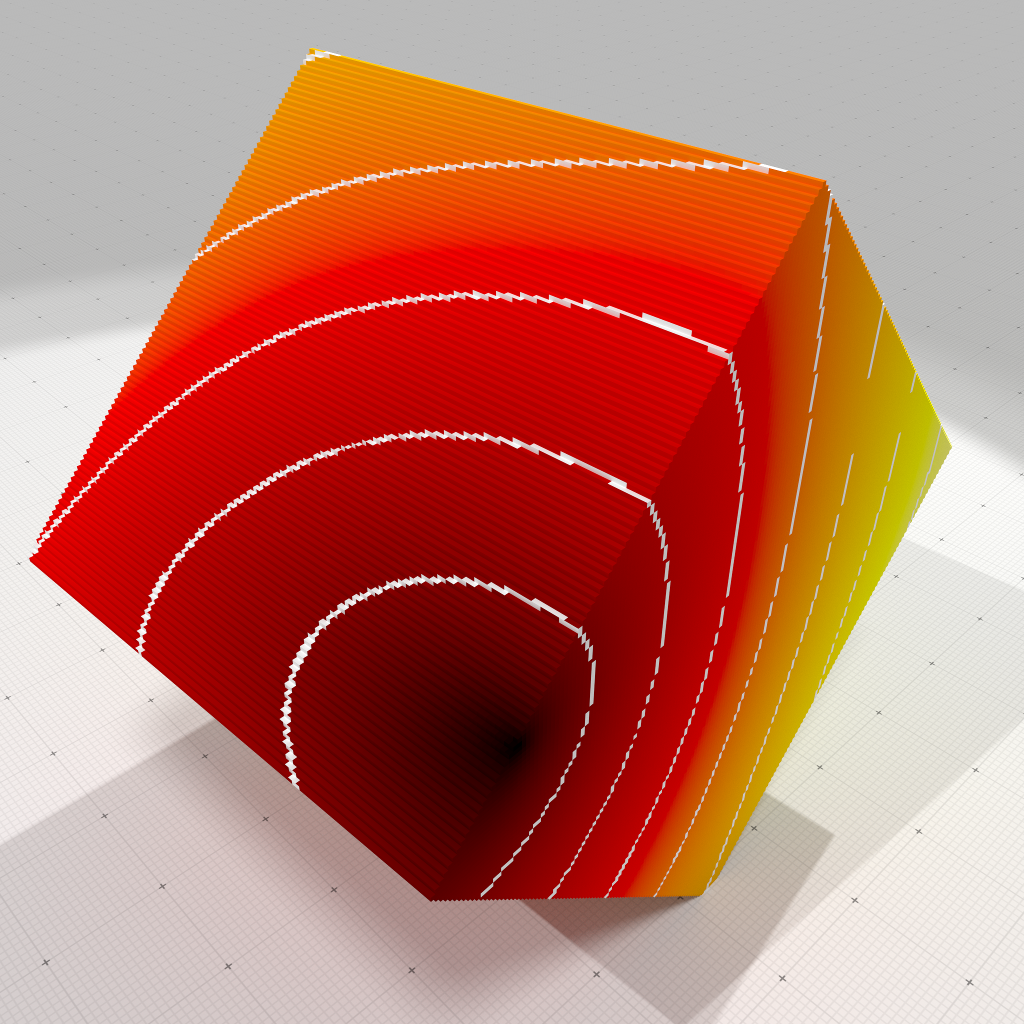
\includegraphics[width=6.8cm]{images/Feature/cubeIsoback}
    \end{center}}
    \caption{Diffusion de chaleur sur un objet digital induit par un opérateur laplacien discret dans la formulation du calcul extérieur discret. Un effet d'escalier apparaît sur les résultats.
      \label{fig:staircase}}
\end{figure}

\subsection{Estimation de singularités par l'analyse en espace d'échelle de la
courbure}%
\label{sec:applications:feature:II}
%
Nous allons décrire un nouvel estimateur de singularités \cite{SMI2015} en
étudiant les estimateurs de courbures par intégration présentés précédemment
(\RefSection{sec:estimators:volume}). Nous allons fixer la résolution $h$ d'une
forme $\DigShape \subset \Z^d$ et considérer la taille de la sphère
d'intégration $R$ comme paramètre de l'espace d'échelle. Ce changement de rayon
de boule d'intégration fera varier le résultat obtenu par notre estimateur de
courbure (\RefFigure{fig:curvature-scale-3d}). Nous parlons ici d'analyse en
espace-échelle de nos estimateurs, le paramètre étant le rayon de la boule.

\begin{figure}[ht]{
    \begin{center}
      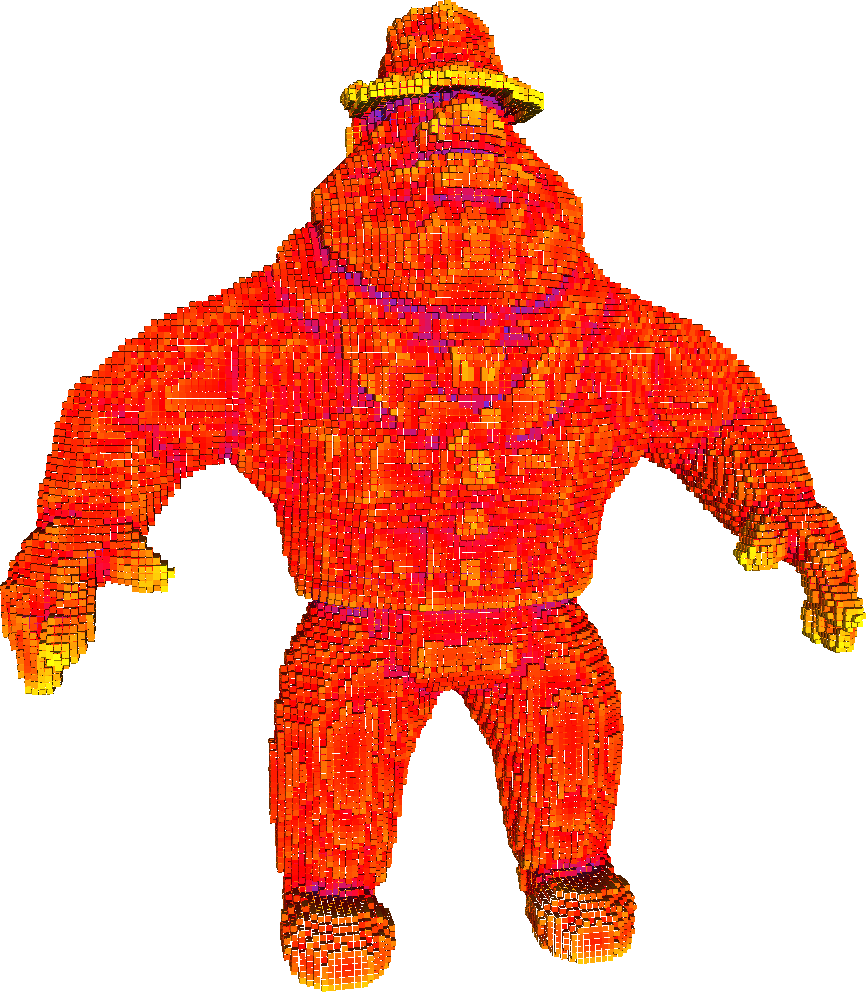
\includegraphics[width=3.2cm]{images/Curvature/MeanAl_4}
      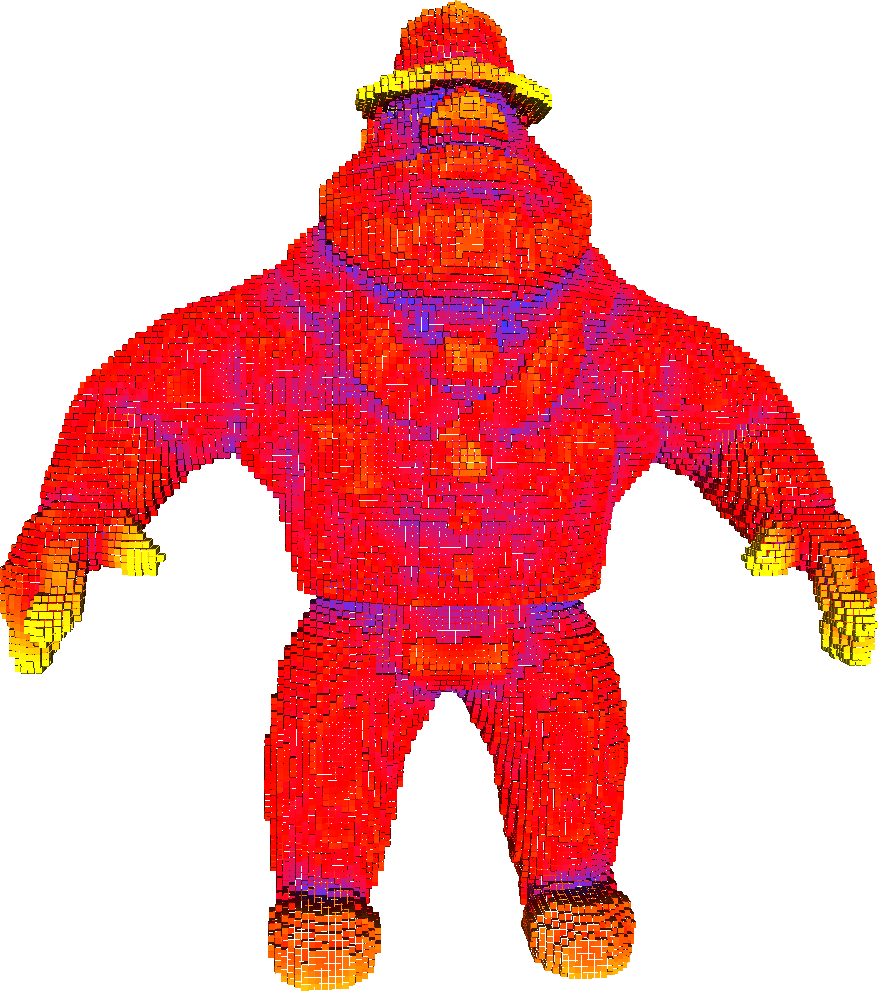
\includegraphics[width=3.2cm]{images/Curvature/MeanAl_7}
      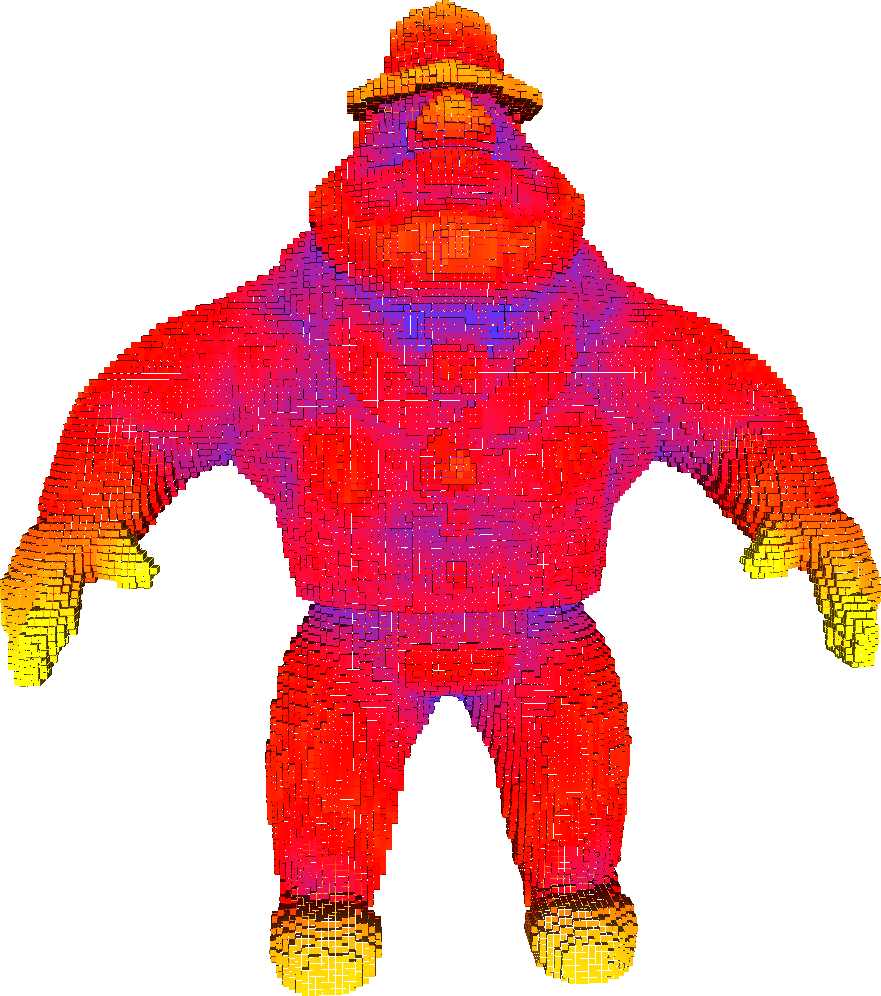
\includegraphics[width=3.2cm]{images/Curvature/MeanAl_14}
      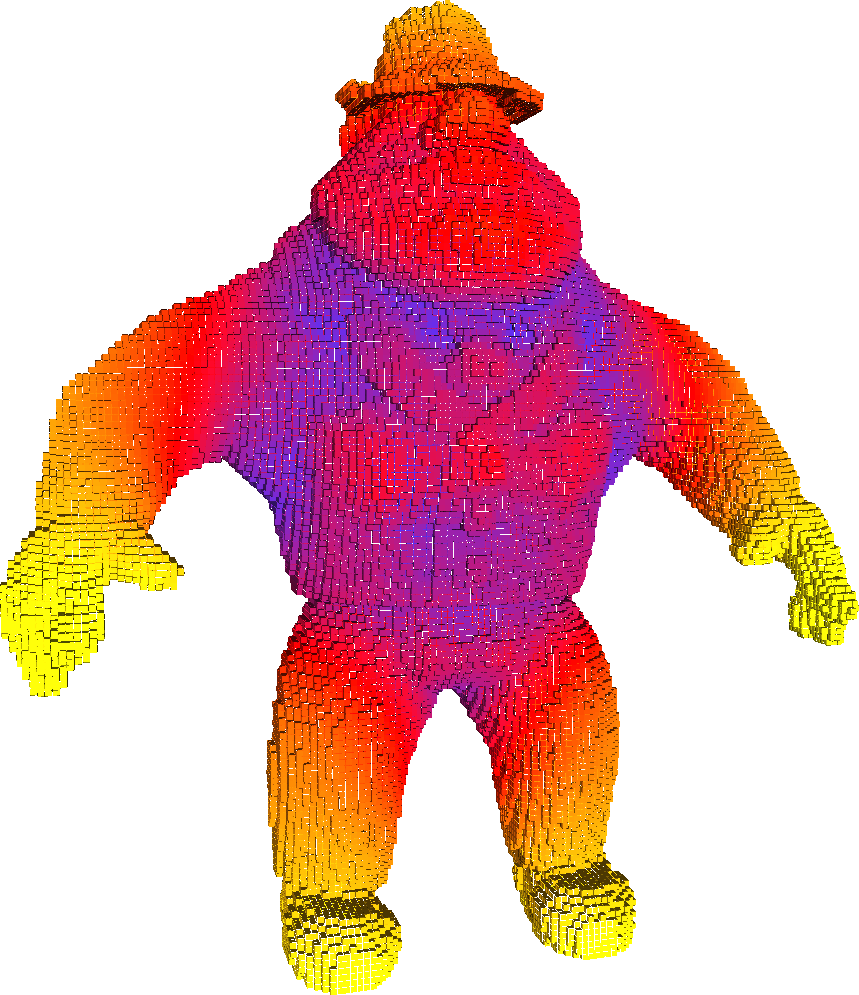
\includegraphics[width=3.2cm]{images/Curvature/MeanAl_30}
      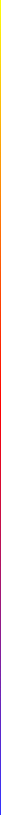
\includegraphics[width=0.1cm,height=3.6cm]{images/YMTB6W}
    \end{center}}
    \caption{Courbure moyenne en utilisant la \RefDefinition{def:digital-3d-mean-curvature}
      pour différents rayons de boule : $4$, $7$, $14$ et $30$.
      \label{fig:curvature-scale-3d}}
\end{figure}

% Dans un premier temps, nous allons faire quelques rappels, puis nous étudierons
% les spécificités en espace-échelle ces estimateurs.
%
% \subsubsection{Rappels et préliminaires}
% \label{sec:applications:feature:II:rappels}
%
% Rappels:
%
% \RefDefinition{def:pottmann-2d-3d-mean} :
% \begin{equation*}
%   \CurvT{R}(\Shape,x) \EqDef \frac{3\pi}{2R} - \frac{3A_R(x)}{R^3},
%   \quad \MeanCurvT{R}(\Shape,x) \EqDef \frac{8}{3R} - \frac{4V_R(x)}{\pi R^4}.
% \end{equation*}
%
% \RefTheorem{theo:pottmann-2d-3d-mean-conv} :
% \begin{equation*}
%   \CurvT{R}(\Shape,x) = \Curv(\Shape,x) + O(R),
%   \quad \MeanCurvT{R}(\Shape,x) = \MeanCurv(\Shape,x) + O(R).
% \end{equation*}
%
% Définitions~\ref{def:ii-2d-3d-mean} et \ref{def:ii-3d-princ} :
% \begin{align*}
%    \CurvH{R}(Z,p) &\EqDef \frac{1}{h} \left( \frac{3 \pi}{2 R_d}
%     - \frac{3 A_{R_d}(p)}{{R_d}^3} \right),\\
%    \MeanCurvH{R}(Z,p) &\EqDef \frac{1}{h} \left( \frac{8}{3 R_d}
%     - \frac{4V_{R_d}(p)}{{\pi R_d}^4} \right),\\
%    \PrincCurvH{1}{R}(Z,p) &\EqDef \frac{1}{h} \left( \frac{6(\hat{\lambda}_2
%     - 3\hat{\lambda}_1)}{\pi {{R_d}}^6} + \frac{8}{5{{R_d}}} \right),\\
%    \PrincCurvH{2}{R}(Z,p) &\EqDef \frac{1}{h} \left( \frac{6(\hat{\lambda}_1
%     - 3\hat{\lambda}_2)}{\pi {{R_d}}^6} + \frac{8}{5{{R_d}}} \right).
% \end{align*}
%
% Théorèmes~\ref{theo:ii-2d-3d-mean-conv} et \ref{theo:ii-3d-princ-conv} :
% \begin{align*}
%   \CurvH{R}(\DigF{\Shape}{h},p) &= \Curv(X,x) + O(h^{\frac{1}{3}}),\\
%   \MeanCurvH{R}(\DigF{\Shape}{h},p) &= \MeanCurv(X,x) + O(h^{\frac{1}{3}}),\\
%   \PrincCurvH{1}{R}(\DigF{\Shape}{h},p) &= \PrincCurv{1}(X,x) + O(h^{\frac{1}{3}}),\\
%   \PrincCurvH{2}{R}(\DigF{\Shape}{h},p) &= \PrincCurv{2}(X,x) + O(h^{\frac{1}{3}}).
% \end{align*}
%
\subsubsection{Analyse en espace d'échelle de $\CurvT{R}(x)$ et $\MeanCurvT{R}(x)$}%
\label{sec:applications:feature:II:analyse}

\begin{figure}[ht]{
      \begin{center}
          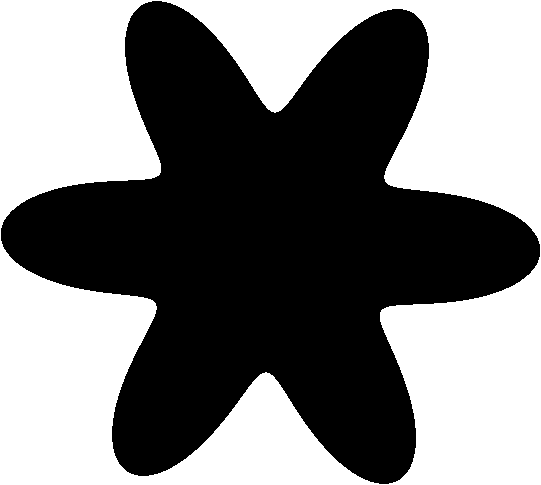
\includegraphics[width=2cm]{images/Flower}
          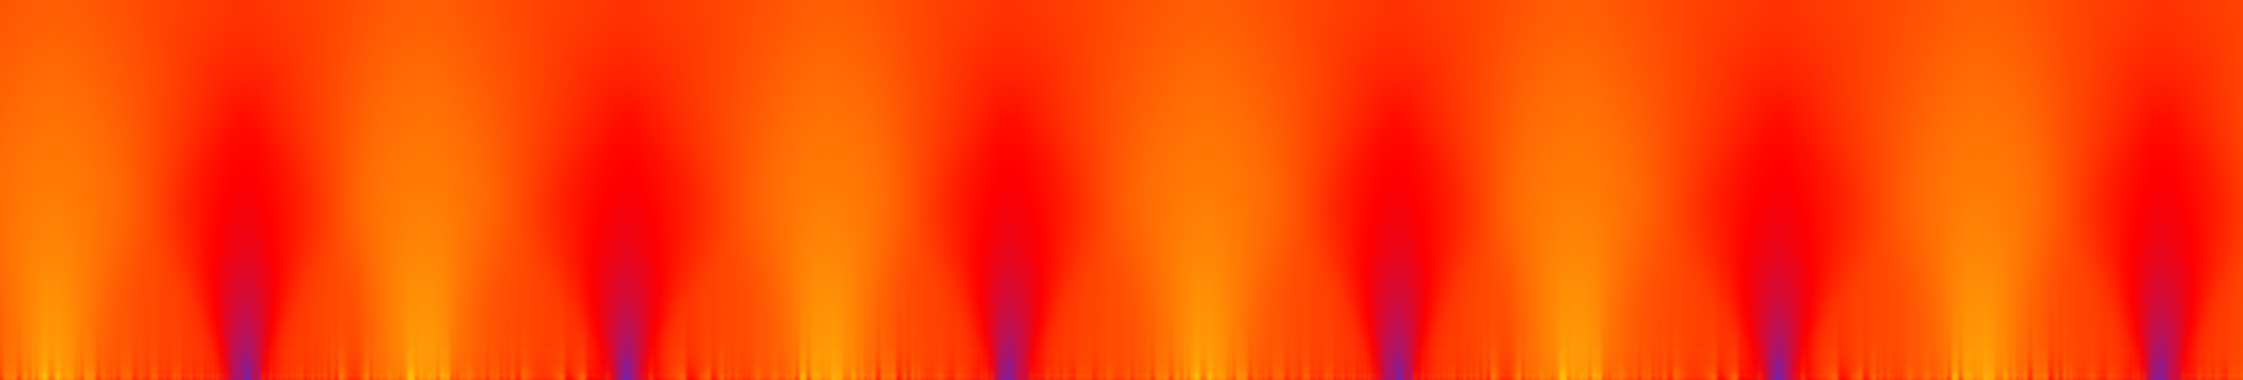
\includegraphics[width=11.7cm]{images/ScaleSpace_Flower}
      \end{center}}
%
      \caption[Analyse en espace d'échelle de la courbure en fonction du rayon sur la forme digitale 2D de \Flower]
      {\emph{À gauche :} forme digitale 2D de \Flower. \emph{À droite :}
      Association des valeurs de courbure sur le bord digital de la forme
      \Flower en utilisant la \RefDefinition{def:digital-2d-curvature} (abscisse) pour différentes
      tailles de boules $R$ (ordonnée, de haut en bas). Les couleurs correspondent
      aux valeurs de courbures: du bleu (courbure la plus petite) au jaune (courbure
      la plus grande).\label{fig:curvature-scale-2d}}
\end{figure}

Nous proposons alors d'étudier le comportement des estimateurs digitaux par
intégration lorsque nous réduisons le rayon de la boule pour une forme et une
résolution donnée. La \RefFigure{fig:curvature-scale-2d} nous montre les
variations de courbure en fonction du rayon de la boule lorsqu'il décroît (de
haut en bas sur la figure) pour l'objet \Flower. Nous nous apercevons que
certaines caractéristiques ne sont perceptibles que dans un certain intervalle de
rayons (les zones bleues par exemple) tandis que d'autres vont s'étendre (les
zones rouges par exemple). Plus généralement, les points autour de singularités
ont une valeur de courbure qui tend à fortement varier en fonction du rayon de
la boule alors que les points autour de zones lisses sont relativement
insensibles au rayon. Pour analyser ce comportement en espace d'échelle, nous
proposons de classifier les points de notre forme en trois catégories :
\featedge (correspondant à des points non-$C^1$), \featsmooth ($C^3$ et
suffisamment lisse) et \featflat (courbure nulle).


Plus formellement :
%
\begin{definition}
  %
  Pour tout point $\vx$ sur le bord d'une forme euclidienne $\Shape$ de $\R^2$
  (\respp $\R^3$), nous définissons \emph{l'estimateur en espace d'échelle de zones
  caractéristiques} $\FeatDD(R)$ (\resp $\FeatTD(R)$) tel que :
  %
  \begin{equation}
  	\FeatDD(R) \EqDef \frac{3 \pi}{2 R} - \frac{3 A(R,\vx)}{R^3},
  	\quad \FeatTD(R) \EqDef \frac{8}{3 R} - \frac{4 V(R,\vx)}{\pi R^4} \,,
  \end{equation}
  %
  où $R$ -- le paramètre de l'espace d'échelle -- est le rayon de la boule
  euclidienne centrée au point $\vx$, $A(R,\vx)$ est l'aire (en 2D) et $V(R,\vx)$ est
  le volume (en 3D) de l'intersection entre la boule et la forme $\Shape$.
  %
  \label{def:feature-estimator}
\end{definition}
%
Dans la suite, nous supposons que l'objet $\Shape$ a un bord $C^3$ par
morceaux, \cad qu'il est lisse avec des singularités. Nous allons détailler
le cas sur une partie lisse de cet objet, puis sur une singularité.
%
\paragraph{Cas lisse.}
%
Dans le cas lisse, \cad lorsque $\dS$ est $C^3$ au point $\vx$, il
apparaît clairement que $\FeatDD(R)$ et $\FeatTD(R)$ sont exactement les
estimateurs de courbures de la \RefDefinition{def:pottmann-2d-3d-mean}.

\begin{figure}[ht]
{\scriptsize
\begin{center}
  \begin{overpic}[width=4cm]{figures/II_kernels_smooth}
    \put(46,51){$\vx$}
    \put(7,10){$\Shape$}
    \put(58,57.5){$R_n$}
    \put(62.5,62){$\iddots$}
    \put(69,67){$R_1$}
    \put(78,76){$R_0$}
  \end{overpic}
\end{center}
}
\end{figure}

Puisque nous sommes dans les mêmes conditions que le
\RefTheorem{theo:pottmann-2d-3d-mean-conv}, nous savons que :
%
\begin{equation}
\FeatDD(R) = \CurvT{}(R,\vx) = \Curv(\vx) + O(R),
\quad \FeatTD(R) = \MeanCurvT{}(R,\vx) = \MeanCurv(\vx) + O(R) \,,
\end{equation}
%
lorsque $R$ décroît vers zéro. Alors $\FeatDD(R)$ nous donne un terme constant
qui est la courbure au point $\vx$.


Nous avons changé la notation car lorsque $\FeatDD(R)$ est sur une singularité,
la valeur retournée n'est plus uniquement liée à la courbure au point $\vx$.
%
\paragraph{Singularité.}

Considérons désormais que le point $\vx$ est localisé sur une singularité de
$\dS$ :
%
\begin{definition}{\fakeTitle{\RefTheoremFake{12}{Pottmann2009}}}
  %
  Soit $\Shape$ une forme euclidienne de $\R^2$ (\respp $\R^3$) avec
  un bord $C^3$ par morceaux, et soit $\vx \in \dS$ une singularité. Alors, si
  $\alpha_0$ est l'angle entre les deux demi-tangentes au point $\vx$ et si
  $\Curv_{-}$ et $\Curv_{+}$ sont les courbures limites à gauche et à droite,
  nous avons:
  %
  \begin{align}
  	A(R,\vx) &= \frac{\alpha_0 R^2}{2} - \frac{\Curv_{-} + \Curv_{+}}{6}R^3 + O(R^4),\\
  	V(R,\vx) &= \frac{2 \alpha_0R^3}{3} - \frac{\pi(\MeanCurv_{-} + \MeanCurv_{+})}{8}R^4 + O(R^5) \,.
  \end{align}
  %
\end{definition}
%
Alors, $\FeatDD(R)$ et $\FeatTD(R)$ sont des fonctions du rayon de la
boule $R$ et de l'angle $\alpha_0$ :
%
\begin{align}
	\FeatDD(R) &= \frac{3}{2} \frac{1}{R} ( \pi - \alpha_0 )
             + \frac{\Curv_{-} + \Curv_{+}}{6} + O(R),\\
	\FeatTD(R) &= \frac{8}{3} \frac{1}{R} ( 1 - \frac{\alpha_0}{\pi} )
             + \frac{\MeanCurv_{-} + \MeanCurv_{+}}{2} + O(R) \,.
  \label{eq:feature-estimator-singularity}
\end{align}
%
$\FeatDD(R)$ nous donne un monôme en $R$ d'exposant $-1$ dont le coefficient est
dépendant de l'angle $\alpha_0$.

\begin{figure}[ht]
{\scriptsize
\begin{center}
  \begin{overpic}[width=6cm]{figures/II_kernels_edge2}
    \put(47,39.5){$\alpha_0$}
    \put(51,30){$\vx$}
    \put(7,1){$\Shape$}
    \put(56.5,42){$R_n$}
    \put(59,45){$\iddots$}
    \put(64,49){$R_1$}
    \put(70,55){$R_0$}
  \end{overpic}
\end{center}
}
\end{figure}

\begin{figure}[ht]
\begin{center}
  {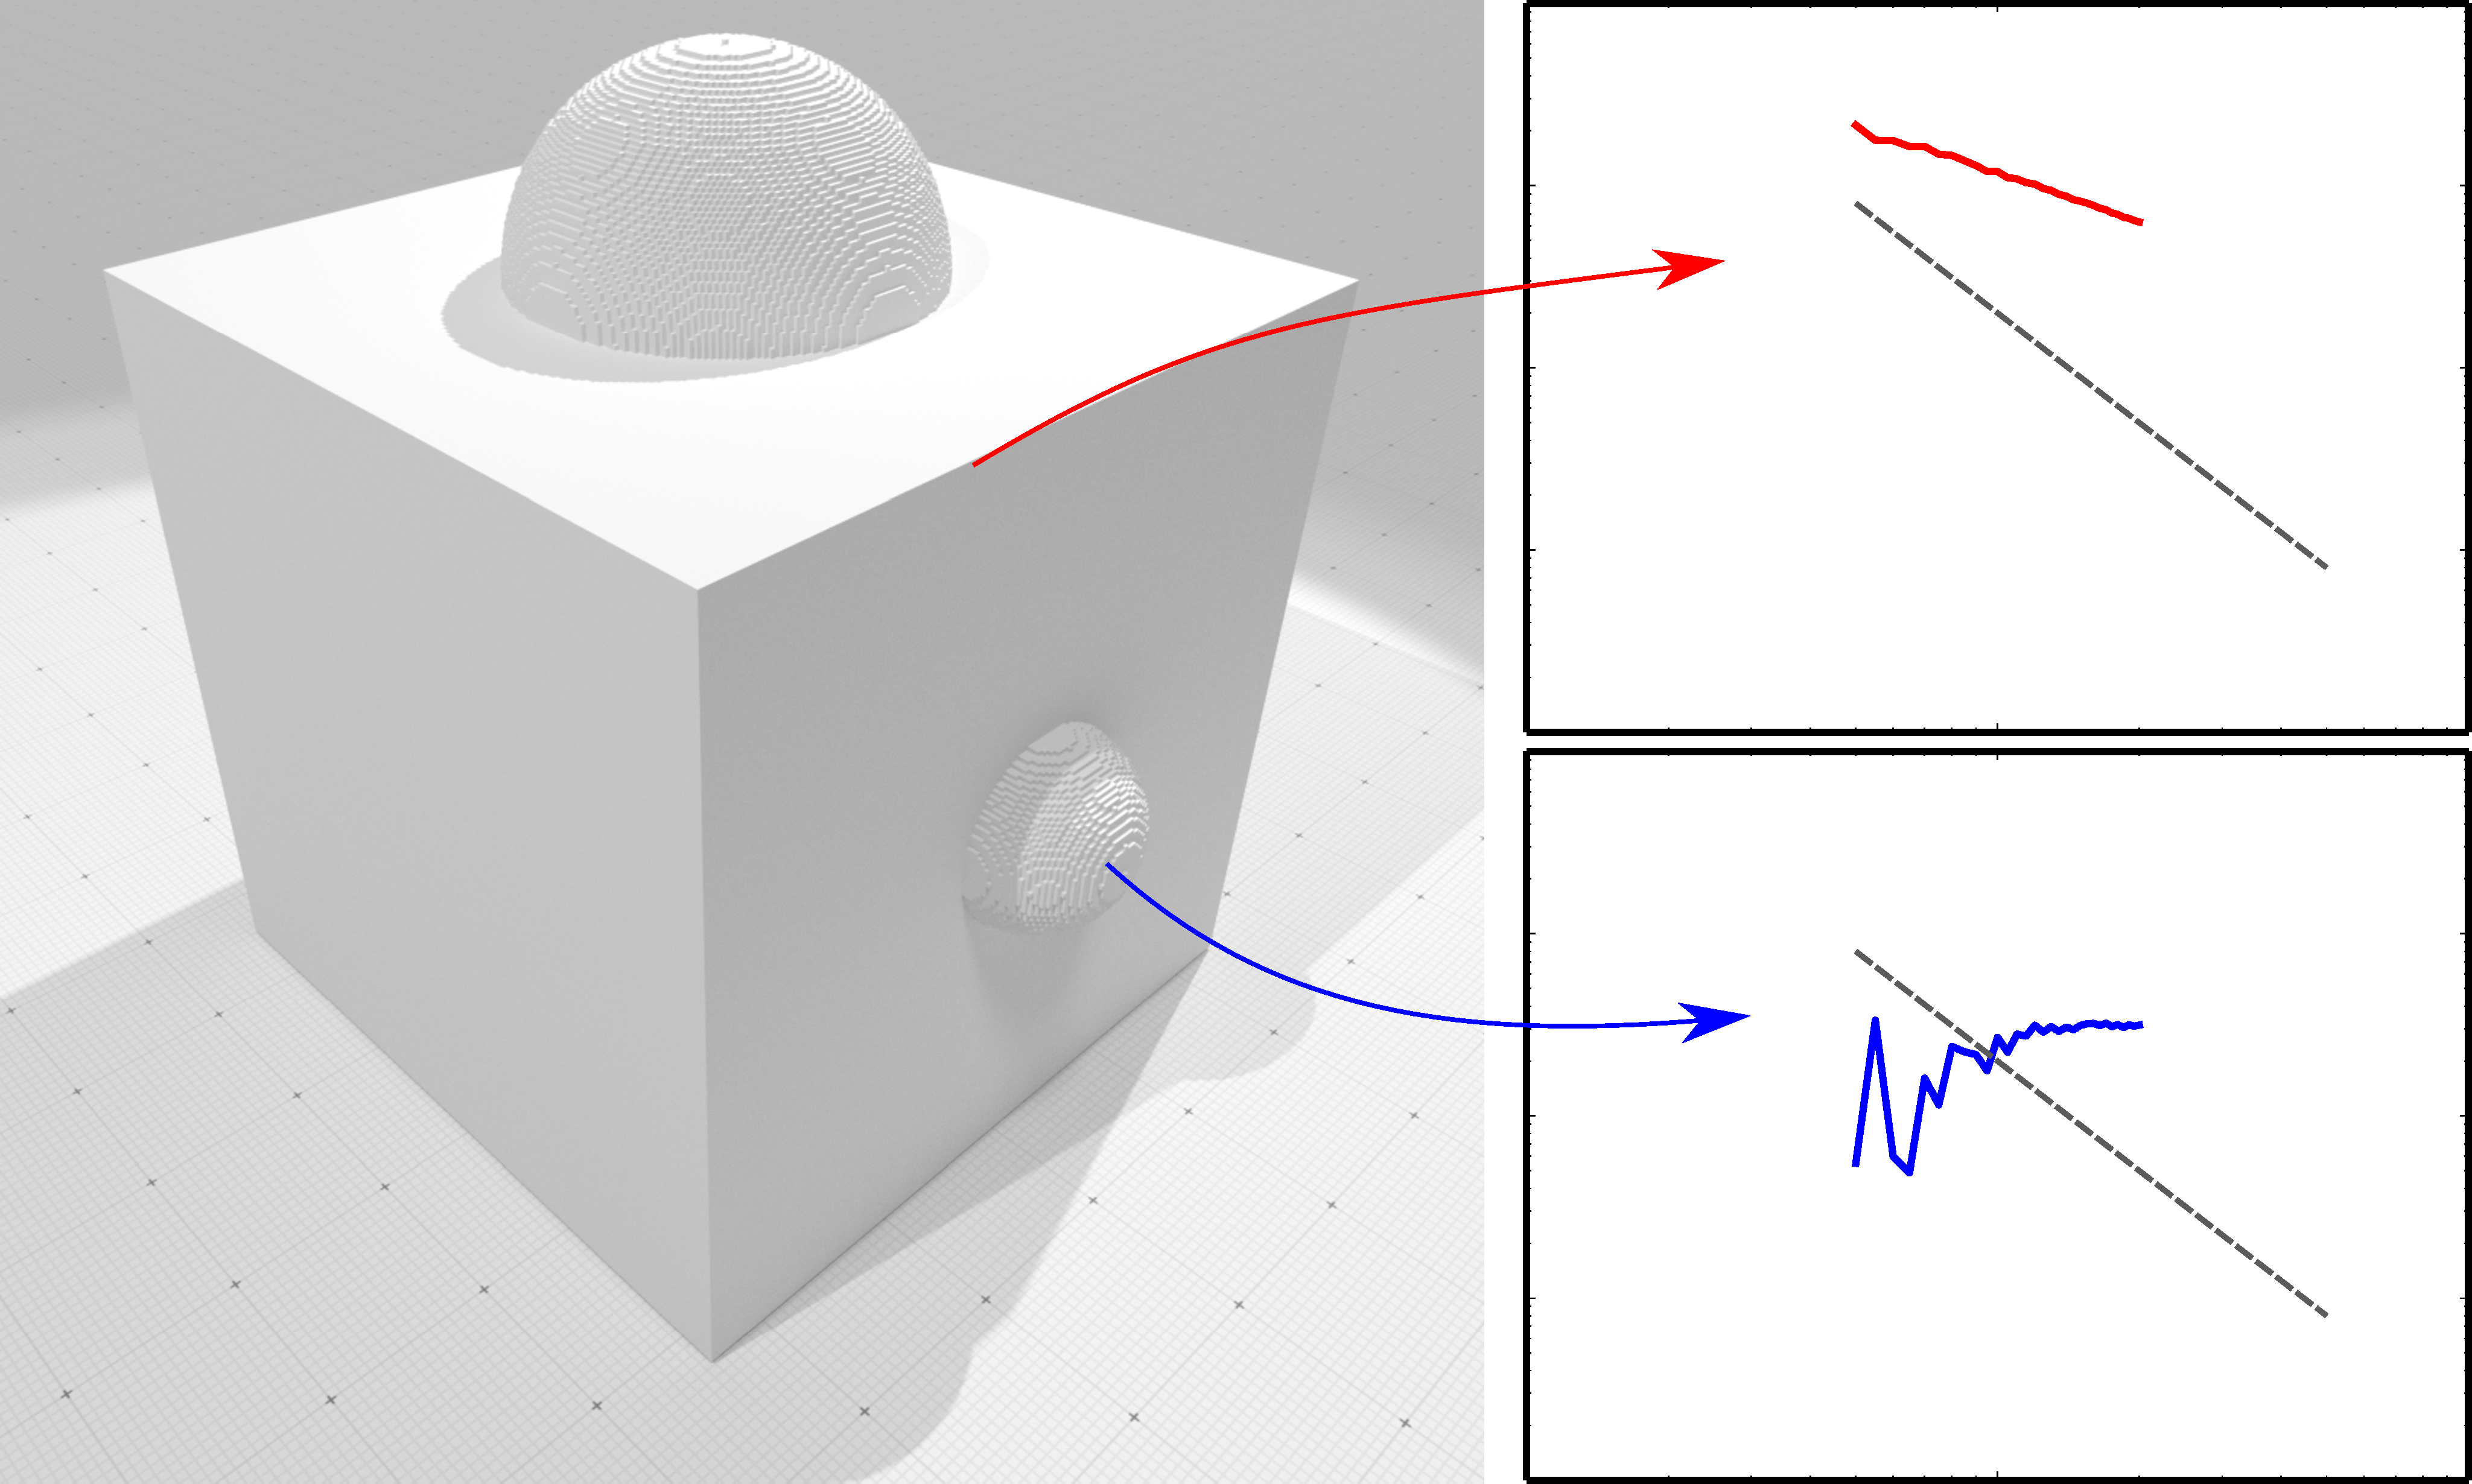
\includegraphics[width=8cm]{figures/CubeSpherePlot_ES_NoColor}}
  %
  \caption{Graphes (en échelle logarithmique) des valeurs de $\FeatTD(R)$ (sur
  l'axe des ordonnées) pour deux points de l'objet
  \CubeSphere en fonction du rayon de la boule (décroissant, de droite à gauche,
  sur l'axe des abscisses).\label{fig:CubeSpherePlot_ES_NoColor}}
  %
\end{center}
\end{figure}

En conclusion, $\FeatDD(R)$ a deux comportements distincts lorsque nous sommes
sur un point d'une surface lisse ou lorsque nous sommes sur une singularité de
la surface. Lorsque le rayon $R$ décroît sur une surface lisse, l'estimateur de
caractéristique nous retourne la courbure au point $\vx$, \cad une valeur
constante. Sur une singularité, l'estimateur de caractéristique nous retourne
une quantité qui croît hyperboliquement lorsque $R$ décroît (donc linéairement
en échelle logarithmique), comme le montre la
\RefFigure{fig:CubeSpherePlot_ES_NoColor}. Il est à noter que pour éviter des
problèmes avec les parties concaves, nous prenons la valeur absolue de
$\FeatDD(R)$.

Les définitions et résultats précédents portent sur des objets euclidiens lisses $\Shape \in
\R^d$, nous devons également nous intéresser au cadre des objets digitaux.
%
\subsubsection{Influence de la discrétisation}%
\label{sec:applications:feature:II:kmax}
%
Lorsque nous discrétisons $\Ball{R}{\vx} \cap \DSh$, pour un rayon de boule $R$ donné et un pas
de discrétisation $h$, une infinité de formes euclidiennes $\Shape$ avec
différentes valeurs de courbure au point $\vx$ donnent exactement la même valeur
pour $\AreaC(\DigF{\Ball{R}{\vx} \cap \Shape}{h}, h)$, et donc la même valeur pour $\FeatDD(R)$. Cela est dû à la perte
d'informations de la discrétisation, et le constat est le même en 3D.

\begin{figure}[ht]{\small
  \begin{center}
    \begin{overpic}[width=10cm]{figures/minInterval_min2}
      \put(28,3){$1 / \CurvMax$}
      \put(57,33){$R$}
      \put(0,20.5){$h$}
    \end{overpic}
  \end{center}}
  \caption[Notations de la propriété~\ref{prop:minInterval}]{Effets de discrétisation et notations de la propriété~\ref{prop:minInterval}. Toutes les courbes noires et grises donnent la même discrétisation d'intersection avec $\Ball{R}{\vx}$.
  \label{fig:minInterval}}
\end{figure}

La \RefFigure{fig:minInterval} illustre ceci en nous montrant une valeur de
$\Ball{R}{\vx} \cap \DSh$ (en bleu) pour une valeur de courbure $\CurvMax$
limite de $\Shape$ (en noir) au point $\vx$ pour un rayon de boule $R$ (en
orange) et un pas de discrétisation $h$ donnés. Toutes les courbes ayant une
valeur (absolue) de courbure inférieure à $\CurvMax$ auront exactement la même
valeur de $\Ball{R}{\vx} \cap \DSh$.


Nous nous intéressons alors à déterminer l'ensemble de valeurs (réelles) de courbure au
point $\vx$ qui correspondent à une zone à courbure nulle à cause de la discrétisation. La
courbure maximale qui peut être incorrectement interprétée comme une région à courbure nulle
est donnée par la propriété suivante :
%
\begin{property}
  %
  Soit $\Shape$ une forme euclidienne sphérique de $\R^2$ (\resp $\R^3$), $R$ le
  rayon de la boule et $h$ le pas de discrétisation, pour $\vx \in \dS$, la
  courbure maximale (\resp la courbure moyenne maximale) au point $\vx$
  résultant à la même quantité $\FeatDD(R)$ (\resp $\FeatTD(R)$) que pour une
  forme plate est :
  %
  \begin{equation}
    \CurvMax(R,h) = \frac{2h}{R^2+h^2},
    \quad\left(\text{\resp~} \MeanCurvMax(R,h) = \frac{2h}{R^2+h^2}\right)\,.
  \end{equation}
  %
  \label{prop:minInterval}
\end{property}
\begin{proof}
  %
  La preuve est directe par relation de Pythagore sur la
  \RefFigure{fig:minInterval}. Soit $R$ le rayon de la boule, $h$ le pas de
  discrétisation de la grille, $\CurvMax(R,h)$ le valeur de courbure réelle
  maximale pour laquelle le pas de discrétisation et le rayon de la boule ne
  permettent pas de distinguer par rapport à une courbure nulle :
  %
  \begin{align}
  	{\left(\frac{1}{\CurvMax(R,h)} - h\right)}^2 + R^2 &= {\left(\frac{1}{\CurvMax(R,h)}\right)}^2 \\
    {\left(\frac{1}{\CurvMax(R,h)}\right)}^2 - 2h\left(\frac{1}{\CurvMax(R,h)}\right) +h^2 + R^2 &= {\left(\frac{1}{\CurvMax(R,h)}\right)}^2 \\
    \frac{1}{\CurvMax(R,h)} &= \frac{R^2 + h^2}{2h} \\
  	\CurvMax(R,h) &= \frac{2h}{R^2+h^2}
  \end{align}
  %
  En 3D, le cas limite est une sphère de courbure moyenne $\MeanCurvMax$ et peut
  être réduite à une coupe 2D, ce qui revient à la même conclusion qu'en 2D.
  %
\end{proof}


En conséquence, si $\FeatDD(R)$ est inférieure à $\CurvMax$ (ou $\FeatTD(R)$
inférieure à $\MeanCurvMax$ en 3D) pour un point $\vx$ de $\dS$, nous ne pouvons
décider si $\vx$ est sur une surface très légèrement lisse ou sur une surface
à courbure nulle. À noter que si nous affichons la valeur de $\CurvMax(R,h)$ ou
$\MeanCurvMax(R,h)$ en échelle logarithmique en fonction du rayon choisi $R$,
nous obtenons une droite de pente $-2$. C'est ce que nous observons par exemple
sur la \RefFigure{fig:CubeSpherePlot_F_NoColor} en pointillés gris.


Il apparaît alors clairement que le rayon $R$ (ou l'ensemble de rayons dans le
cas d'une analyse en espace d'échelle) de la boule contrôle la \emph{taille} de
la caractéristique qui sera détectée à cause des artefacts de discrétisation :
une singularité trop petite avec un pas de discrétisation trop faible sera
absorbé par les artefacts de discrétisation.

\begin{figure}[ht]
\begin{center}
  {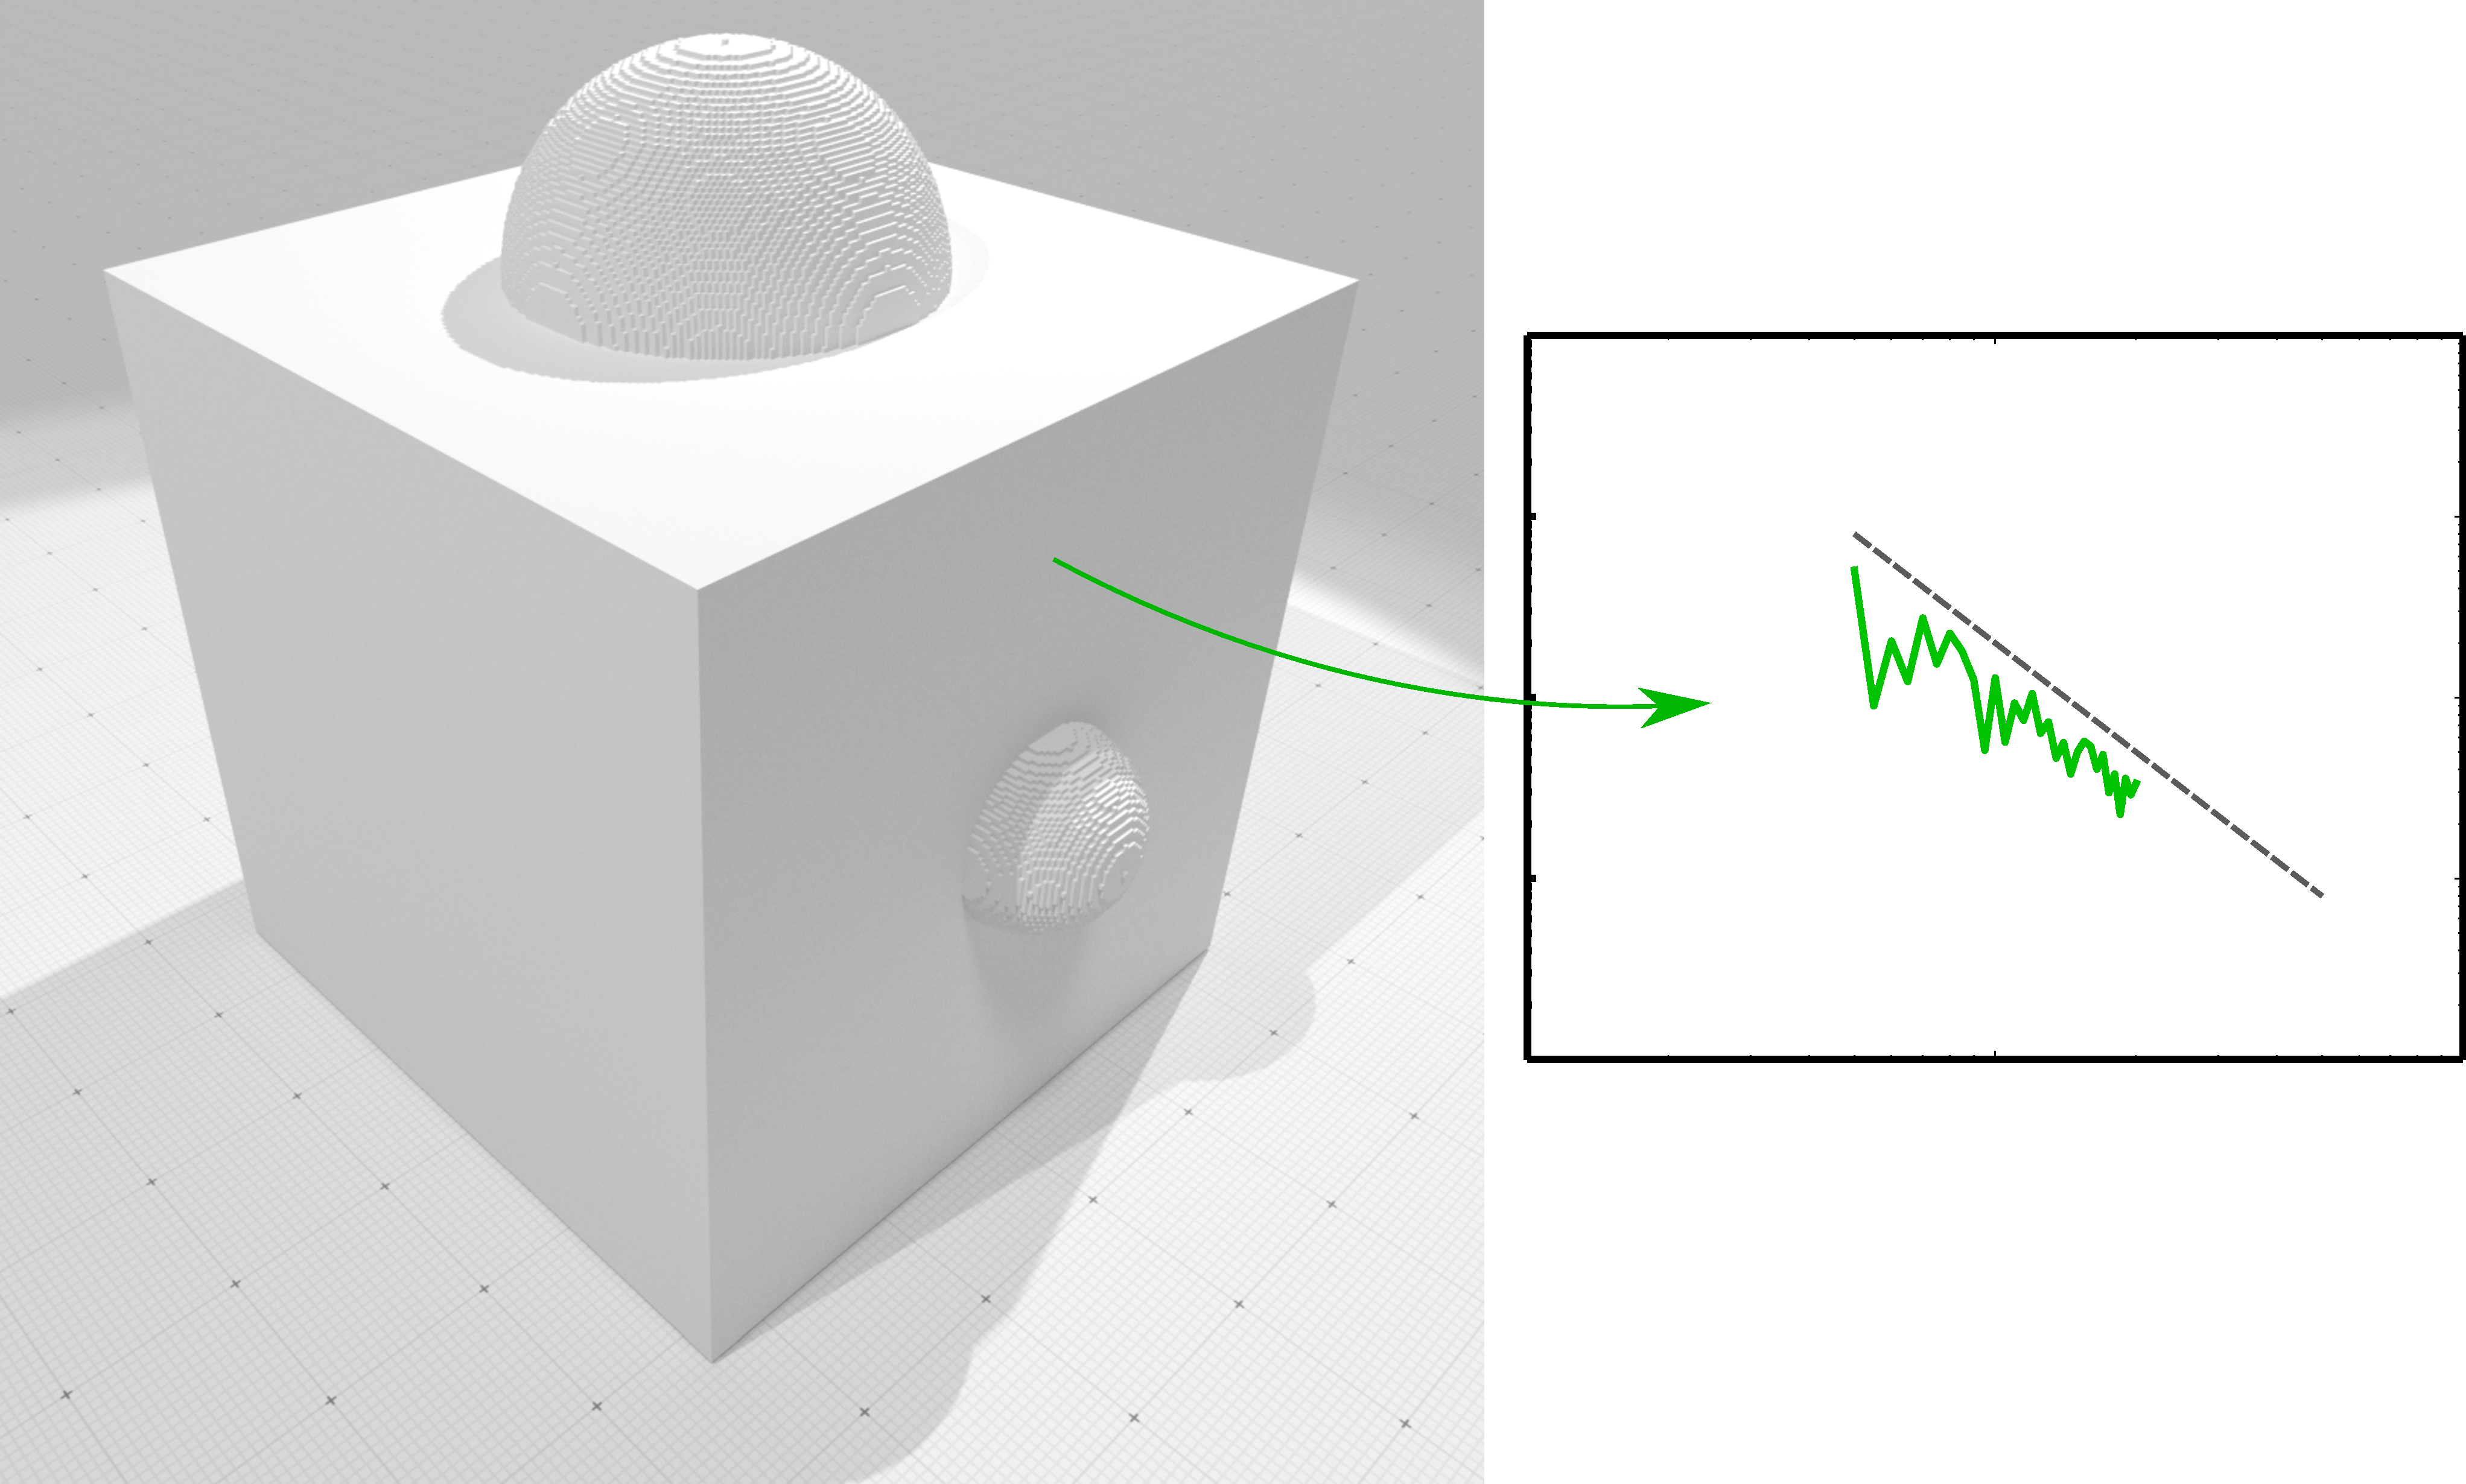
\includegraphics[width=8cm]{figures/CubeSpherePlot_F_NoColor}}
  %
  \caption{Graphe (en échelle logarithmique) des valeurs de $\FeatTD(R)$ (sur
  l'axe des ordonnées) pour un point d'une région à courbure nulle de l'objet
  \CubeSphere en fonction du rayon de la boule (décroissant, de droite à gauche,
  sur l'axe des abscisses).\label{fig:CubeSpherePlot_F_NoColor}}
  %
\end{center}
\end{figure}

Nous pouvons observer les trois cas en espace d'échelle : sur la courbe verte de
la \RefFigure{fig:CubeSpherePlot_F_NoColor}, toutes les valeurs de $\FeatTD(R)$
sont inférieures à $\MeanCurvMax$ (représentées par la droite grise en
pointillés), ce qui est caractéristique des régions à courbure nulle. Sur la
courbe rouge de la \RefFigure{fig:CubeSpherePlot_ES_NoColor}, toutes les valeurs
de $\FeatTD(R)$ sont au dessus de $\MeanCurvMax$ et de pente $-1$, ce qui est le
comportement attendu pour les singularités. Sur la courbe bleue de la
\RefFigure{fig:CubeSpherePlot_ES_NoColor}, les valeurs de $\FeatTD(R)$ sont au
dessous de $\MeanCurvMax$ seulement pour de petits rayons $R$, ce qui laisse
supposer que ces rayons sont \emph{trop petits} pour capturer la régularité de
la surface. Pour des rayons plus grands, les valeurs de $\MeanCurvMax$ sont
supérieures à $\FeatTD(R)$ et sont constants, ce qui est le comportement attendu
pour les régions lisses. Comme décrit dans le
\RefSection{sec:applications:feature:II:classification}, la classification
finale considérera uniquement les rayons dont les valeurs de $\FeatDD(R)$
sont supérieures à $\CurvMax$ (ou $\FeatTD(R)$ et $\MeanCurvMax$ en 3D); les
points au dessous seront considérés comme des régions à courbure nulle ou des «
données incorrectes ».
%
\subsubsection{Classification basée sur la distance aux modèles linéaires}%
\label{sec:applications:feature:II:classification}
%
Nous avons deux comportements distincts exploitables en espace d'échelle pour
notre classification :
%
\begin{itemize}
   \item nous pouvons détecter les zones à courbure nulle/« données incorrectes » en
         utilisant $\CurvMax$ ou $\MeanCurvMax$;
   \item lorsque les valeurs sont considérées comme « correctes », \cad dont les valeurs sont au dessus de
         $\CurvMax$, nous pouvons alors distinguer si nous sommes sur une surface
         lisse ou sur des singularités lorsque $R$ décroît.
\end{itemize}
%
Ces comportements sont exactement les mêmes en 2D et en 3D, ce qui suit peut
être appliqué indifféremment pour $\FeatDD(R)$ comme $\FeatTD(R)$.


Pour un intervalle de rayons décroissants $R_i$, $0 \leq i \leq n$, nous
calculons l'estimateur de singularités $\DigFeatDD(R)$ (la version
digitale de $\FeatDD(R)$) au point $\vp \in \Boundary{\DigShape}$, avec $\DigShape = \DSh$).


Dans un premier temps, nous supprimons les « données incorrectes » du graphe de
la fonction $\DigFeatDD(R)$ (\cad tous les points dont la valeur de courbure est
inférieure à \CurvMax). S'il n'y a plus suffisamment de données (trop de valeurs
sous \CurvMax), nous classifions ce point comme \featflat. Sur toutes les images
suivantes, la couleur verte sera assignée aux zones classifiées \featflat
(\RefFigure{fig:inversion} par exemple). S'il reste assez de données, nous
calculons une approximation aux moindres carrés (\anglais{least square fitting})
des données, en échelle logarithmique, d'un modèle linéaire de pente en $0$
(fonction constante que nous nommerons « modèle \featsmooth », l'ordonnée étant
inconnue) et d'un modèle linéaire de valeur de pente de $-1$ (« modèle \featedge »,
l'ordonnée est également inconnue, voir
\RefEquation{eq:feature-estimator-singularity}).


Pour un modèle linéaire donné de pente $\gamma$ fixée, la distance entre le modèle
linéaire $e_\gamma$ et l'ensemble $\{\DigFeatDD(R_i), ..., \DigFeatDD(R_j)\}$ (pour
$n$ valeurs de rayons $R_i$, $0 \leq i \leq n$) est donné par :
%
\begin{equation}
  \label{eq:distance-modele-lineaire}
  e_\gamma(\DigFeatDD(R_i), ..., \DigFeatDD(R_j))= \min_{b\in \mathbb{R}}
  \left ( \sum_{k=i}^j (Y_k - \gamma X_k + b)^2\right)\,,
\end{equation}
%
avec $X_k=\log (R_k)$ et $Y_k=\log(\DigFeatDD(R_k))$. Puisque nous minimisons une
somme de termes quadratiques, la valeur de $b^*$ pour laquelle
l'\RefEquation{eq:distance-modele-lineaire} est minimale est :
%
\begin{equation}
  b^* = \frac{\sum_{k=i}^j ( \gamma X_k - Y_k)}{n}\,.
\end{equation}
%
Si la distance au « modèle \featsmooth » est inférieure que la distance au «
modèle \featedge », nous pouvons classifier le point comme \featsmooth (de
couleur bleu), sinon il correspondra à la classe \featedge (de couleur rouge).


Pour une infinité de petites rayons et un pas de discrétisation $h$, cette
classification capture parfaitement les comportements constants et hyperboliques
des valeurs de courbures, et il décide correctement si le point est une
singularité ou pas.

\subsubsection{Transitions de modèles et classification générale}%
\label{sec:applications:feature:II:transitions}

Lorsque nous traitons des données bruitées, la classification idéale précédente
peut être hautement perturbée si le bruit introduit de grandes valeurs de
courbures dans le profil de courbure pour de petits rayons. En plus de ces
artefacts, pour un ensemble fini de rayons, des transitions de classes peuvent
apparaître. Par exemple, lorsqu'un point est proche d'une singularité, ce point
peut être classifié comme \featedge pour de grands rayons, \featsmooth pour de
plus petits et éventuellement \featflat si la valeur tombe au dessous de
$\CurvMax(R,h)$. Cet effet est illustré sur la \RefFigure{fig:inversion} pour un
point proche d'une singularité.

\begin{figure}
\begin{center}
  {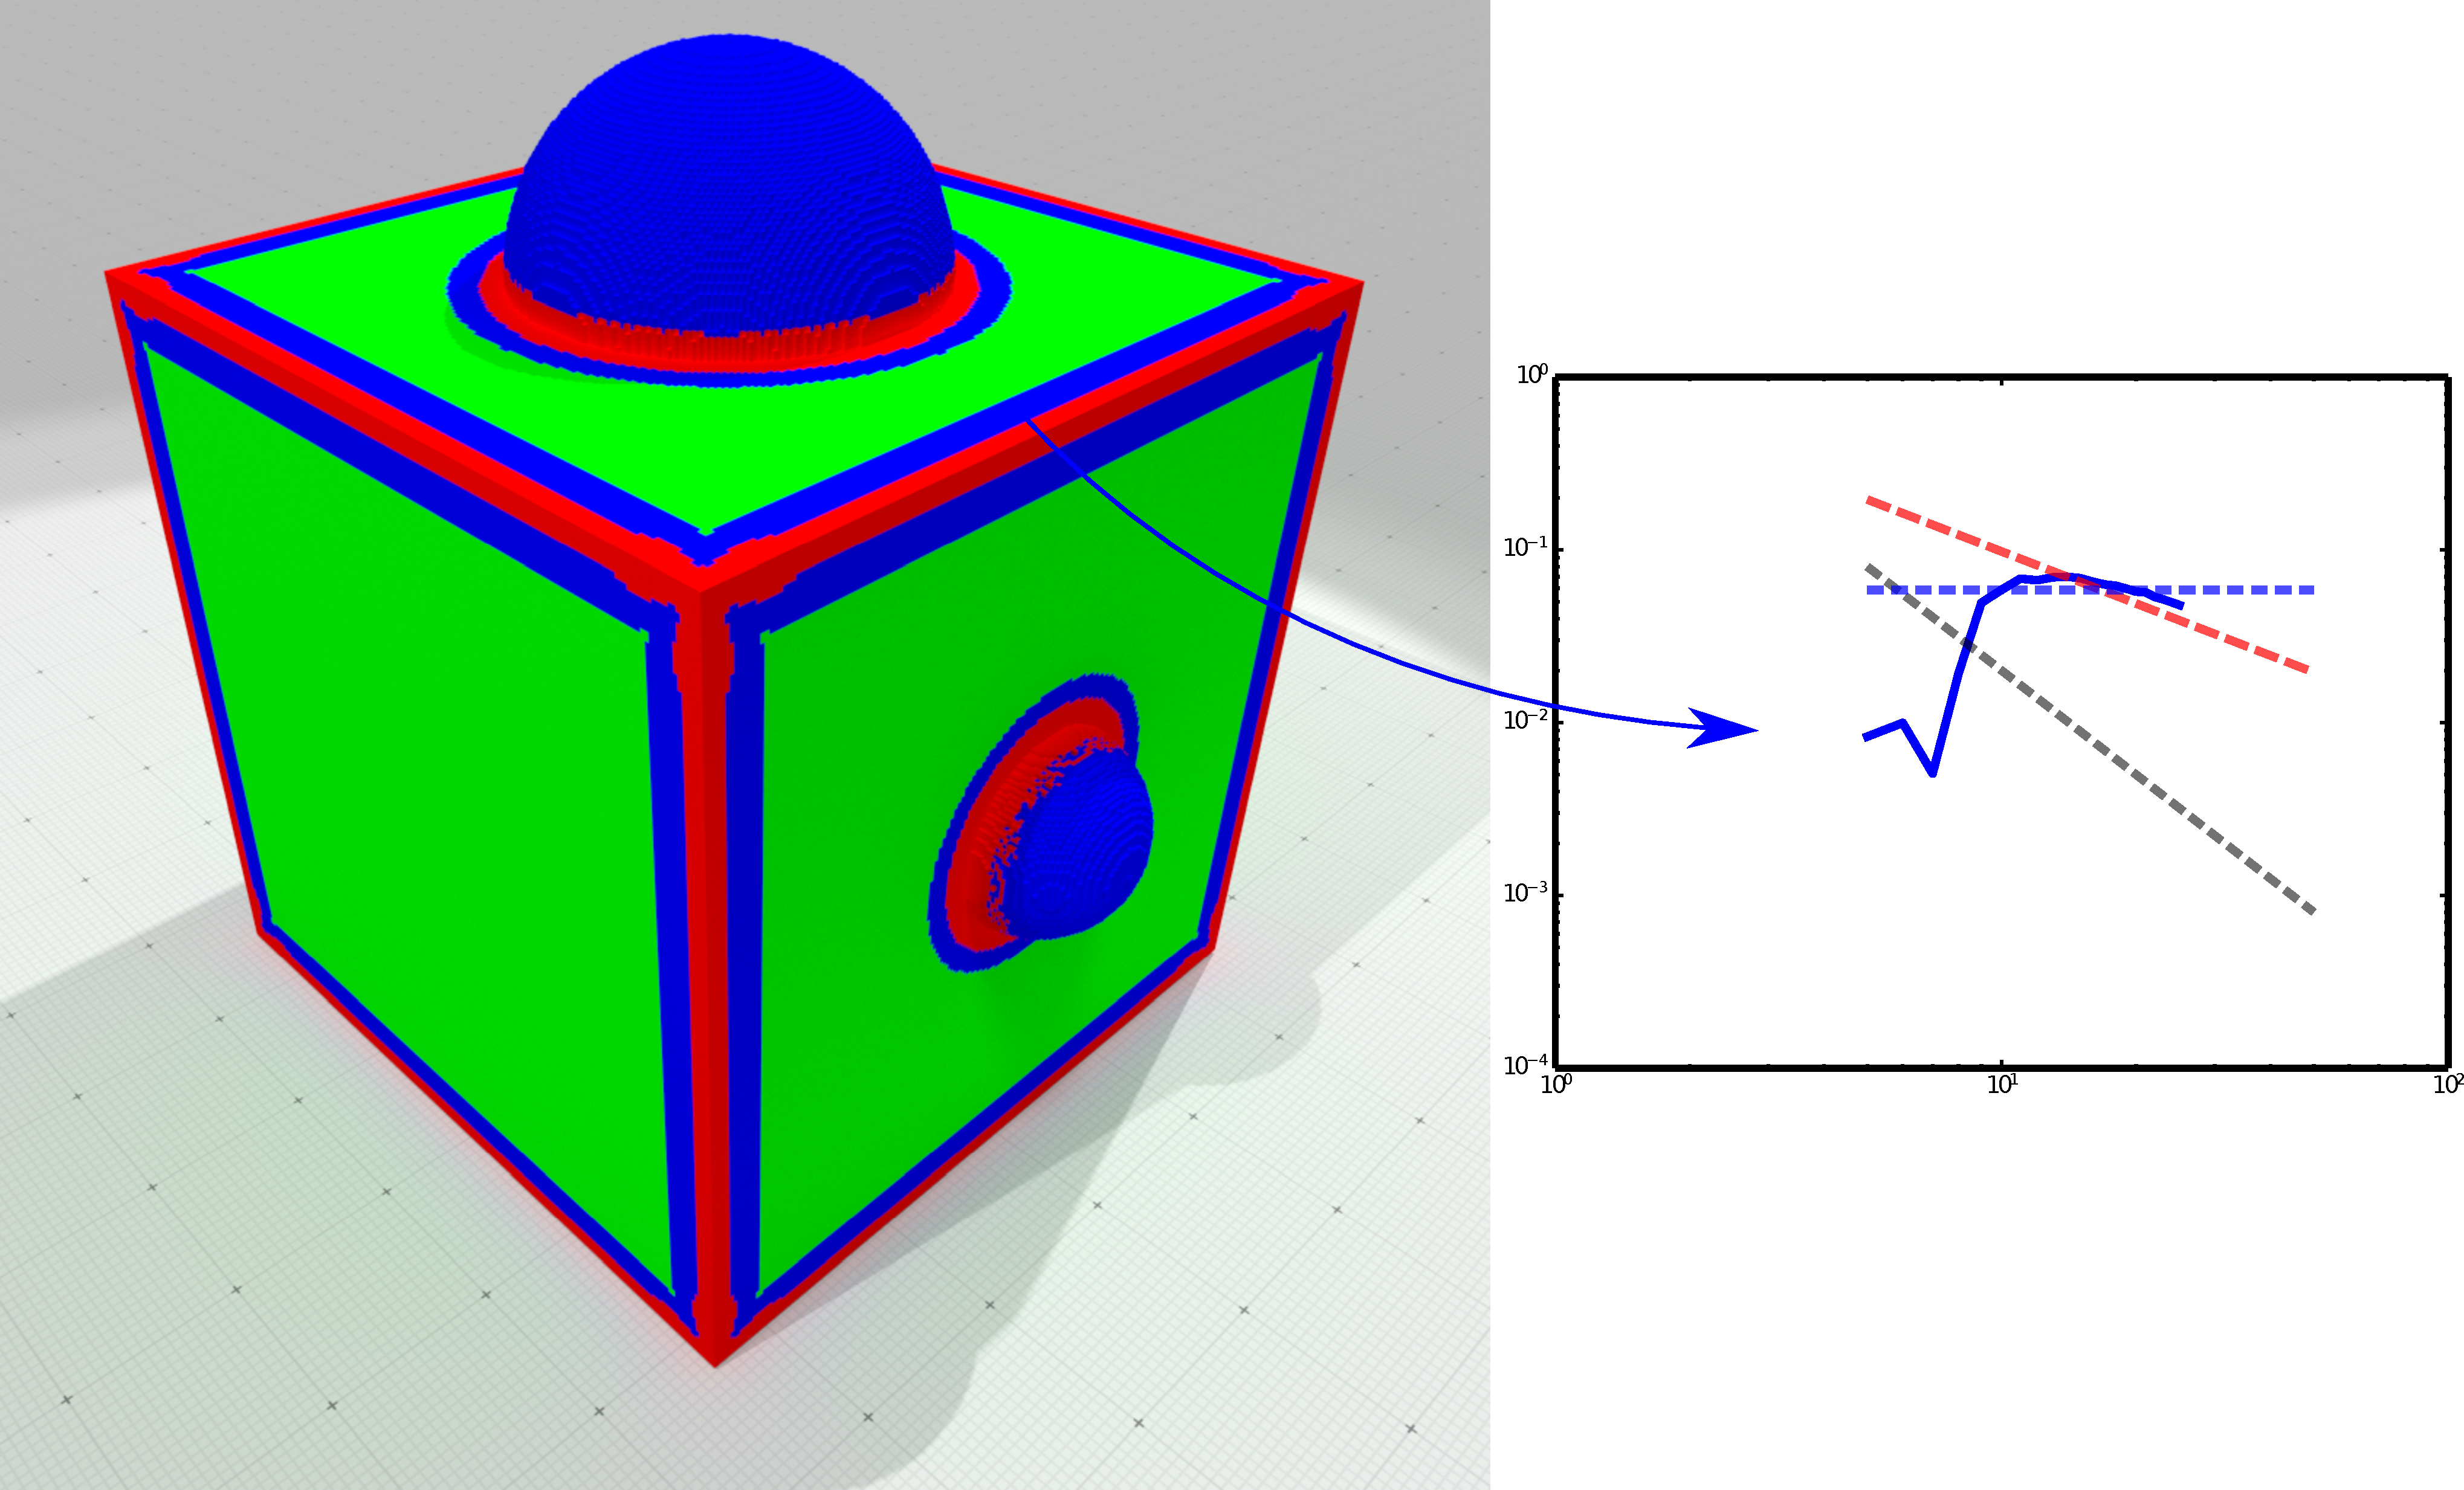
\includegraphics[width=8cm]{figures/CubeSpherePlot_transition}}
  \caption{Graphe de transition de modèles d'un point proche d'une singularité.}
  \label{fig:inversion}
\end{center}
\end{figure}

Afin de reconnaître ce comportement, nous introduisons dans un premier temps un
nouveau modèle linéaire de pente de $-2$ qui correspond à la pente de
$\CurvMax(R,h)$ comme nous l'avons vu précédemment, que nous allons nommer le «
modèle \featflat ». Si la distance au modèle \featflat est inférieure aux
distances aux modèles \featsmooth et \featedge, nous pouvons corriger la
classification en \featflat. Nous pouvons alors évaluer le comportement des
trois distances lorsque le rayon de la boule change. En faisant cela, nous
pouvons évaluer lorsque des transitions opèrent lors des approximations de
modèles linéaires. Si une transition est détectée (voir
\RefFigure{fig:inversion}), nous décidons de classifier le point au modèle dont
la distance est minimale pour le plus large ensemble de rayons.


Plus formellement, nous définissons $l_{\gamma}$ le nombre de rayons dans
l'intervalle $[R_0,R_n]$ pour lesquels la distance $e_\gamma$ au modèle de pente
$\gamma$ (pour $\gamma$ compris dans $\{-2, -1, 0\}$) est minimale (comparée aux
autres).


Finalement, pour un point $\vp$ du bord $\Boundary \DigShape$ de la forme $\DigShape \subset \Z^2$ ou $\Z^3$, nous
définissons notre classification de zones caractéristiques comme suit :
%
\begin{equation}
 C_{\DigShape,\vp}(R_0, R_n) =
  \begin{cases}
      \text{FLAT},         & \text{si } \forall 0 \leq i \leq n,    \DigFeatDD(R_i) < \CurvMax(R_i,h) \\
                           & \text{ou si } l_{-2} > \max( l_{-1}, l_{0} )\\
      \text{SMOOTH},       & \text{si } l_{0}> \max( l_{-1}, l_{-2} )\\
      \text{EDGE},        & \text{sinon.}
  \end{cases}
\end{equation}

\subsubsection{Résultats}%
\label{sec:applications:feature:II:results}

Nous allons désormais tester notre classificateur sur un jeu de données, en 2D comme en
3D. Les comparaisons avec les autres estimateurs sont disponibles dans le
\RefSection{sec:applications:feature:comparison}.


Il est important de noter que le rayon maximal $R_0$ de notre intervalle de
rayons de boule est relié à la plus petite courbure d'une région \featsmooth que
nous souhaitons détecter. Autrement, d'après la \RefProperty{prop:minInterval},
notre estimateur classera avec erreur la zone comme une partie \featflat car les
rayons utilisés ne permettent pas de détecter la géométrie locale de la forme
discrétisée.
%
%\missingfigure{Montrer un exemple de feature avec un range de rayon trop petit}
%
%\missingfigure{Robustesse de II feature}
%
L'autre avantage de notre classificateur est qu'il ne nécessite aucun paramètre
autre que l'intervalle de rayons. De ce fait, il est alors simple de classer des
zones quelle que soit la résolution de la forme. La \RefFigure{fig:feature-octa}
nous montre le résultat de classification pour différentes résolutions de la
forme \OctaFlower : $256^3$, $512^3$ et $1024^3$ et la
\RefFigure{fig:feature-snow} sur l'objet \Bunny ainsi que sur des
micro-structures de neige.
%
Comme pour l'estimation de courbure, un pré-calcul de la taille de la forme
grâce aux segments maximaux pourrait aider à se défaire de ces paramètres de
rayons.

\begin{figure}[ht]
  \begin{center}
    \setlength{\tabcolsep}{1pt}
    \begin{tabular}{c c c}
      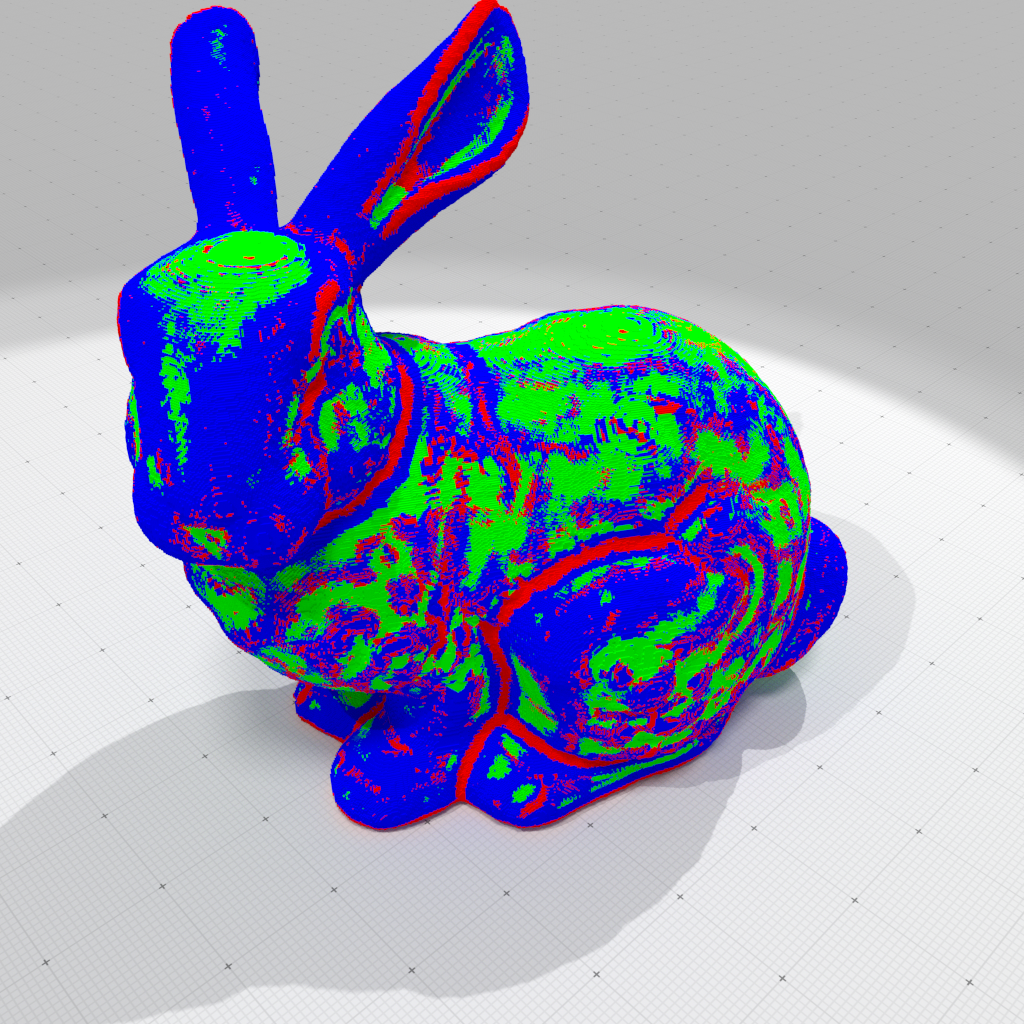
\includegraphics[width=4.5cm]{images/Feature/Bunny_512_II_scale} &
      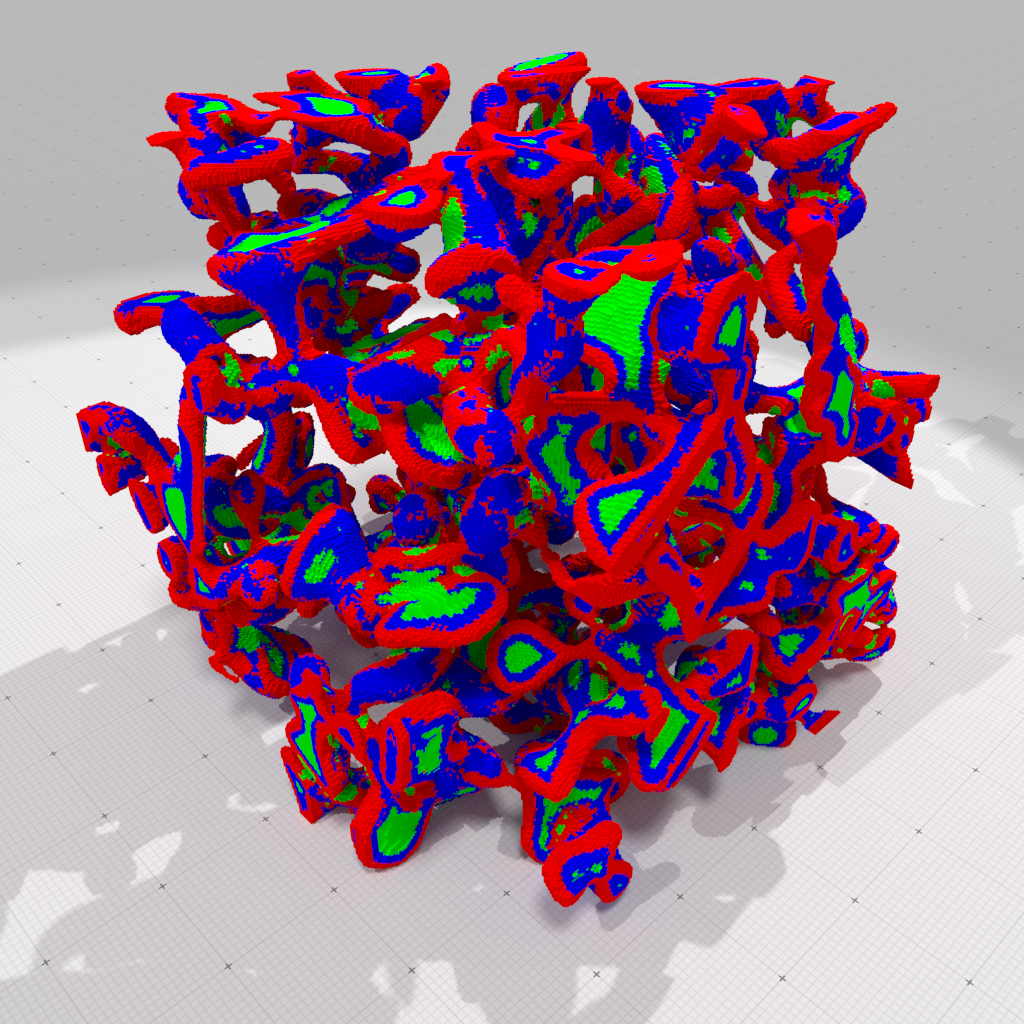
\includegraphics[width=4.5cm]{images/Feature/Snow_I08_II_scale} &
      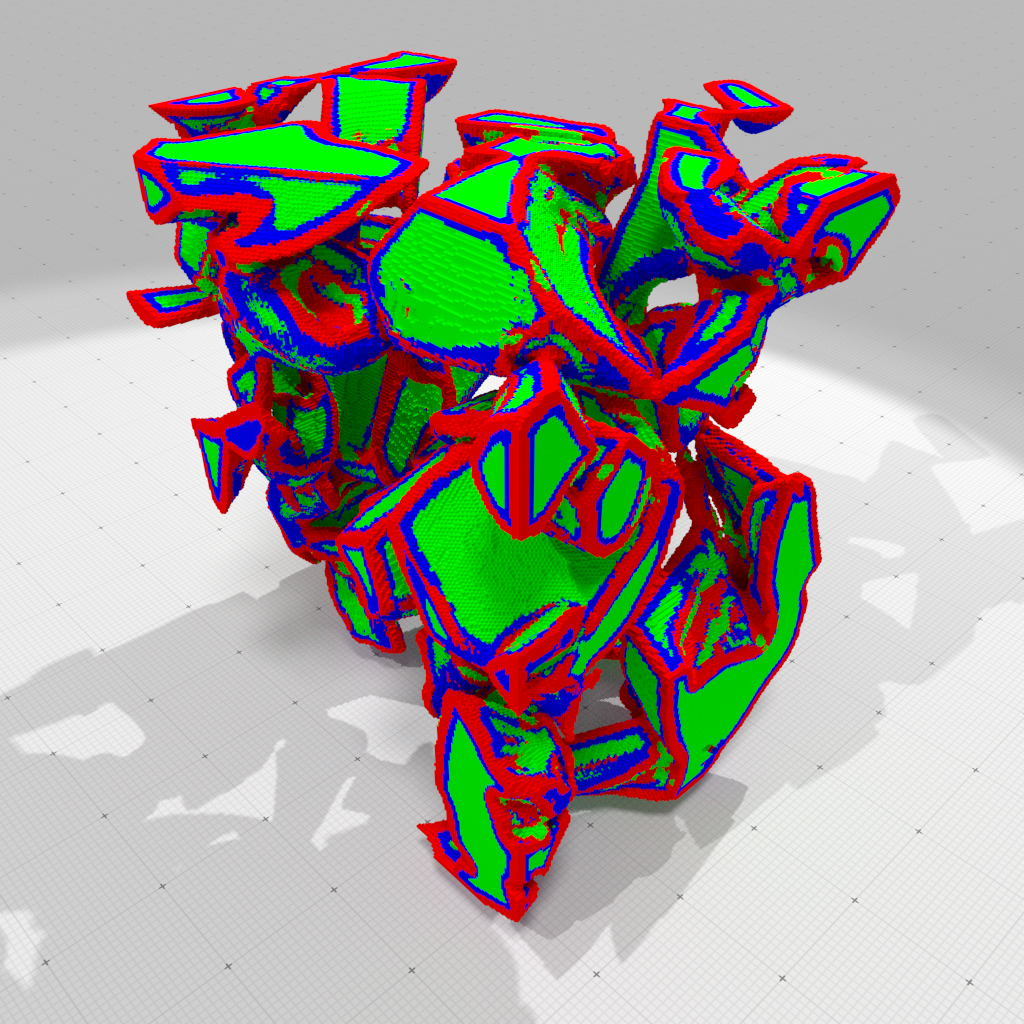
\includegraphics[width=4.5cm]{images/Feature/Snow_E2bis_II_scale} \\
    \end{tabular}
    %
    \caption{Résultat de notre estimateur de singularité sur l'objet \Bunny
    ainsi que des micro-structures de neige obtenues à partir de
    micro-tomographie à rayons X.\label{fig:feature-snow}}
    %
  \end{center}
\end{figure}

\begin{figure}[ht]
  \begin{center}
    \setlength{\tabcolsep}{1pt}
    \begin{tabular}{c c c}
      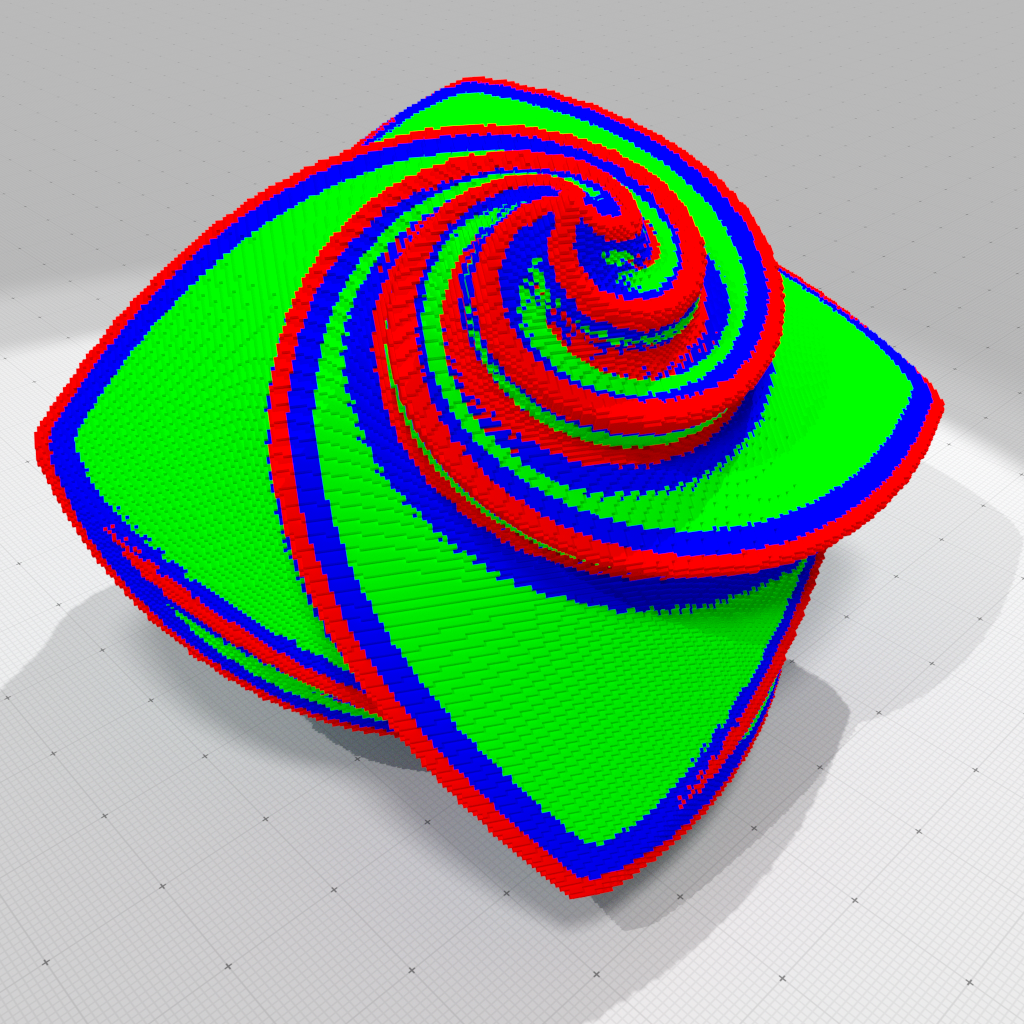
\includegraphics[width=4.5cm]{images/Feature/OctaFlower_256_II_scale} &
      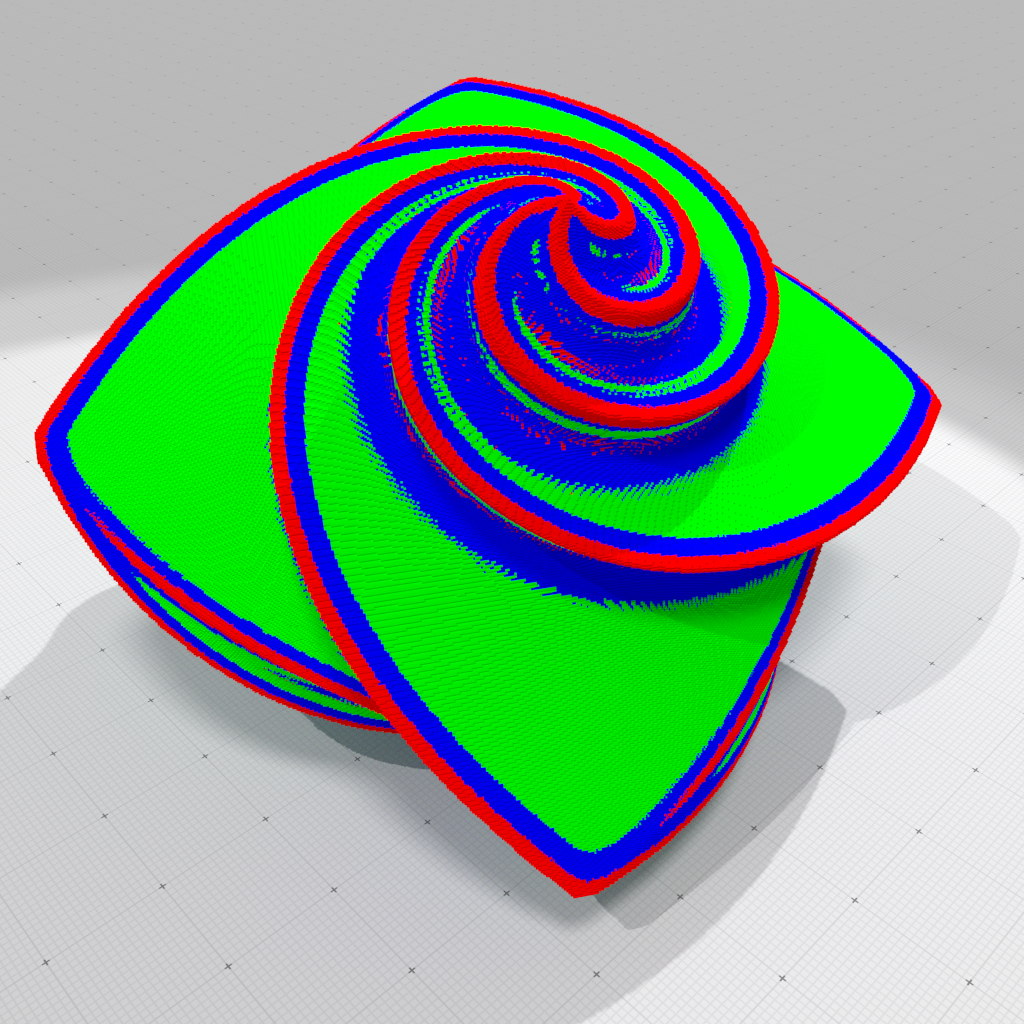
\includegraphics[width=4.5cm]{images/Feature/OctaFlower_512_II_scale} &
      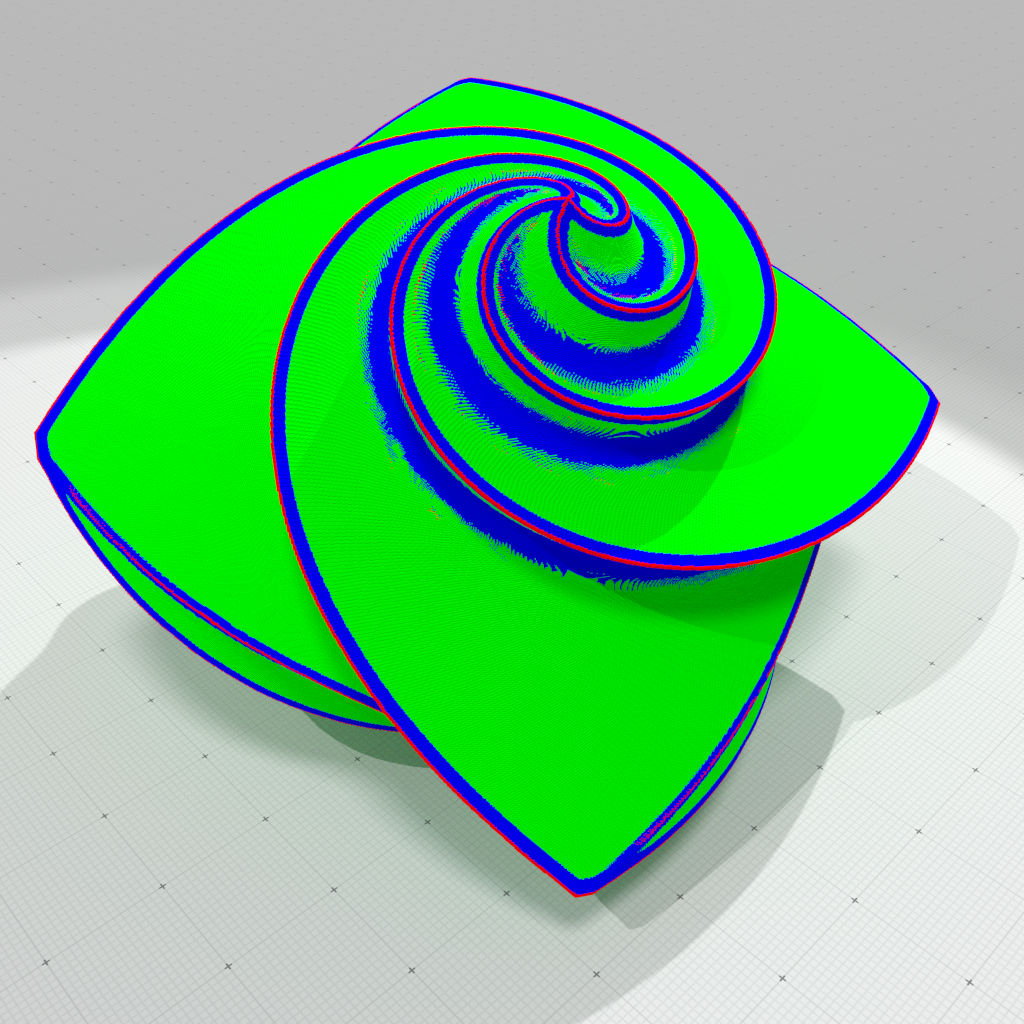
\includegraphics[width=4.5cm]{images/Feature/OctaFlower_1024_II_scale}
    \end{tabular}
    \caption{Résultat de notre estimateur de singularité sur l'objet \OctaFlower à différentes résolutions ($256^3$, $512^3$ et $1024^3$).\label{fig:feature-octa}}
  \end{center}
\end{figure}

\subsection{Comparaison des estimateurs de points caractéristiques}%
\label{sec:applications:feature:comparison}
%
Dans cette section, nous allons comparer qualitativement différents estimateurs
de points caractéristiques les plus représentatifs de l'état de l'art pouvant
s'adapter sur des données digitales. Dans le cadre de notre comparaison, nous
avons mis en œuvre les estimateurs décrits dans le
\RefSection{sec:applications:feature:SOTA} (voir le \RefTable{tab:feature-est}).
Notre comparaison porte sur quatre objets digitaux; deux principalement
utilisés dans le domaine : \Fandisk et \OctaFlower; et deux permettant de mettre
en relief l'importance de l'échelle choisie dans les estimateurs : \SpheresUnion
et \CubeSphere. Ces derniers comportent en effet plusieurs zones
caractéristiques de différentes tailles (\RefTable{tab:feature-objects}).


\begin{table}[h]
  \begin{center}
    \caption{Table des estimateurs de points caractéristiques utilisés pour la comparaison.}
    \label{tab:feature-est}
    \begin{tabular}{@{}lp{2cm}lp{1.2cm}l@{}}
      \toprule
      Méthode & Paramètres & Classification & Espace d'échelle & Robustesse     \\ \midrule
      \cauthors{Clarenz}{Telea2004}   & $R$, $\alpha$, $\beta$  & \multicolumn{1}{c}{\svgNope}   & \multicolumn{1}{c}{\svgNope}   & \multicolumn{1}{c}{\svgYes} \\
      \cauthors{Mérigot}{Merigot2011} & $R$, $r$, $T$           & \multicolumn{1}{c}{\svgNope}   & \multicolumn{1}{c}{\svgNope}   & \multicolumn{1}{c}{\svgYes} \\
      \cauthors{Mellado}{Mellado2012} & $r_{min}$, $r_{max}$    & \multicolumn{1}{c}{\svgNope}   & \multicolumn{1}{c}{\svgNope}   & \multicolumn{1}{c}{\svgYes} \\
      \cauthors{Pauly}{Pauly2003}     & $r_{min}$, $r_{max}$, $\tau_{max}$   & \multicolumn{1}{c}{\svgNope}   & \multicolumn{1}{c}{\svgYes} & \multicolumn{1}{c}{\svgNope}   \\
      \cauthors{Park}{Park2012}       & $r_{min}$, $r_{max}$, $\omega^-$, $\omega^+$, $\tau$ & \multicolumn{1}{c}{\svgYes} & \multicolumn{1}{c}{\svgYes} & \multicolumn{1}{c}{\svgNope}   \\
      Notre méthode                    & $r_{min}$, $r_{max}$ & \multicolumn{1}{c}{\svgYes} & \multicolumn{1}{c}{\svgYes} & \multicolumn{1}{c}{\svgYes} \\ \bottomrule
    \end{tabular}
  \end{center}
\end{table}



\begin{table}[h]
  \begin{center}
    \caption{Table des objets digitaux utilisés pour la comparaison.}
    \label{tab:feature-objects}
    \begin{tabular}{@{}lrrr@{}}
      \toprule
      Object & Résolution (voxels) & \multicolumn{2}{r}{\# éléments de surface (surfels)} \\ \cmidrule(l){3-4}
                     &            & non bruité & bruité \\ \midrule
      \textsc{SpheresUnion}    & $400 \times 200 \times 200$ & $\nombre{265062}$ & $\nombre{640476}$ \\
      \textsc{CubeSphere}     & $200^3$    & $\nombre{262642}$ & $\nombre{855316}$   \\
      \textsc{Fandisk}        & $512^3$    & $\nombre{734658}$ & $\nombre{1832088}$   \\
      \textsc{OctaFlower}     & $512^3$    & $\nombre{692916}$ & $\nombre{1740509}$   \\ \bottomrule
    \end{tabular}
  \end{center}
\end{table}


Nous avons fait le choix d'étudier les paramètres des estimateurs au préalable
afin qu'ils obtiennent de bons résultats sur des formes non bruitées\footnote{Le
bruit utilisé est un bruit de \Kanungo, comme expliqué dans le
\RefSection{sec:kanungo-noise}.}. Afin de montrer l'importance de ces paramètres et
la nécessité d'étudier au préalable la forme pour certains estimateurs, nous
utilisons exactement les mêmes paramètres sur les formes bruitées.


Les \RefFigures{fig:feature-comparative}{fig:feature-comparative-2} montrent les
résultats des estimateurs sur les formes parfaitement
discrétisées\footnote{C'est-à-dire en l'absence de bruit autre que la discrétisation.}
tandis que les
\RefFiguresN{fig:feature-comparative-noise}{fig:feature-comparative-noise-2}
montrent les résultats des estimateurs sur les formes bruitées. Les paramètres
utilisés sont spécifiés dans les légendes des figures.

\begin{figure}[ht]
\begin{overpic}[width=\textwidth,height=.9\textheight]%
  {images/misc/TransparentPixel}
  \put(-5,50){%
    \setlength{\tabcolsep}{1pt}
    \begin{tabular}{l c c c cl}
      \rotatebox{90}{~~~~~~Input data} &
      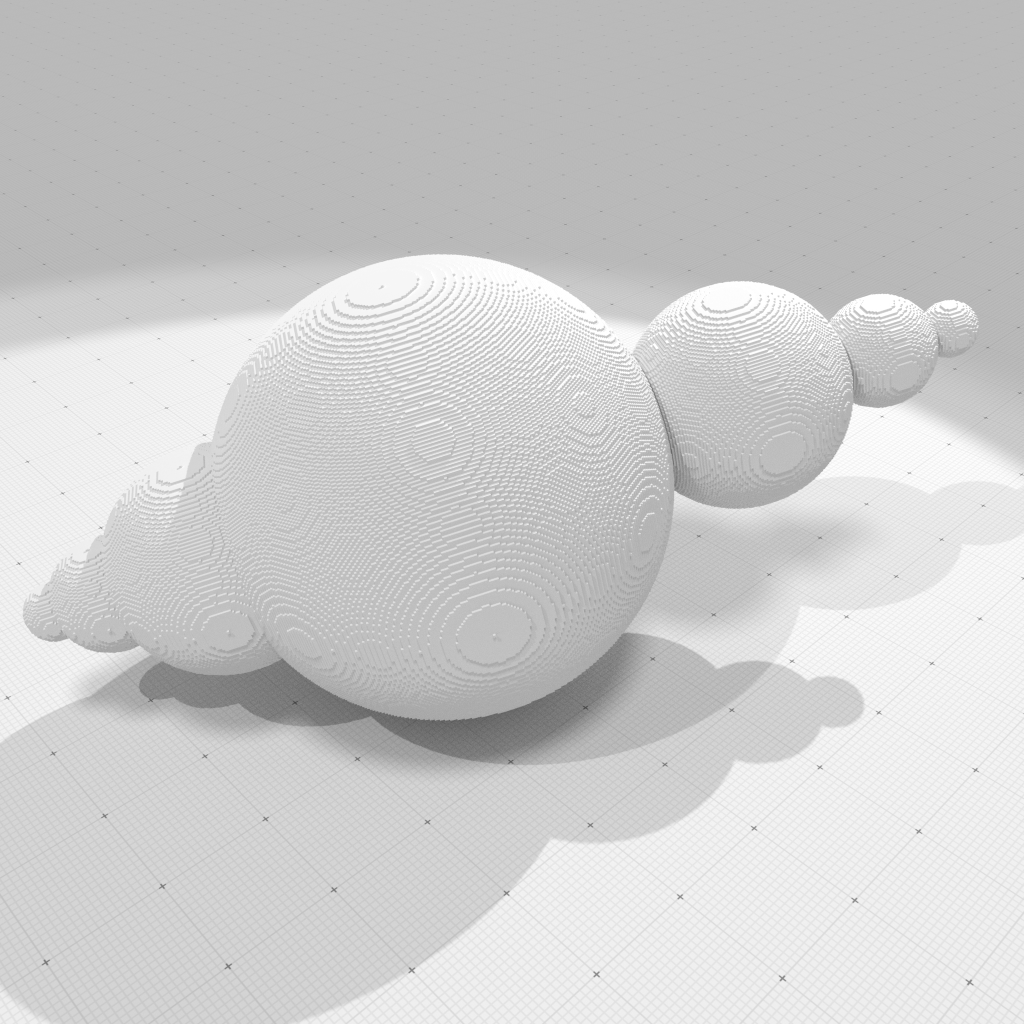
\includegraphics[width=4.0cm]{images/Feature/SphereSphereSphere} &
      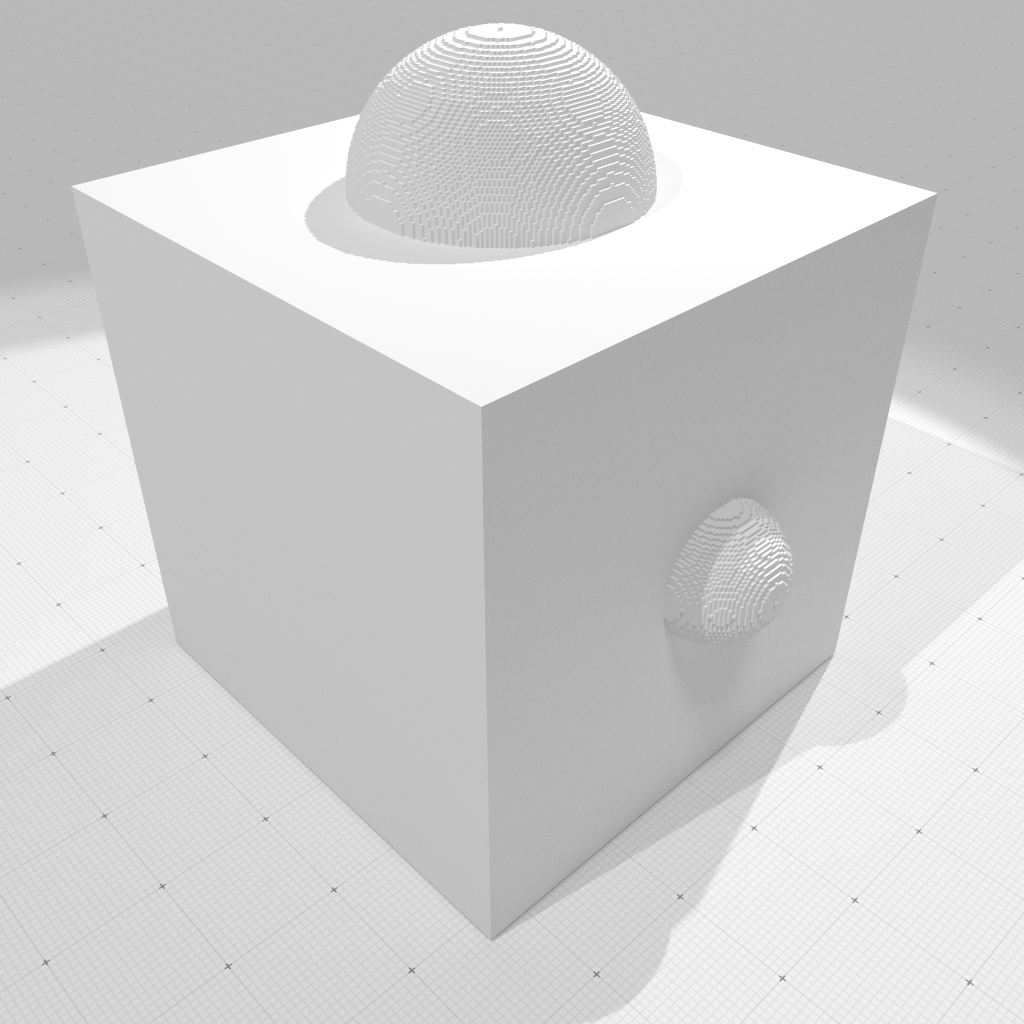
\includegraphics[width=4.0cm]{images/Feature/CubeSphere} &
      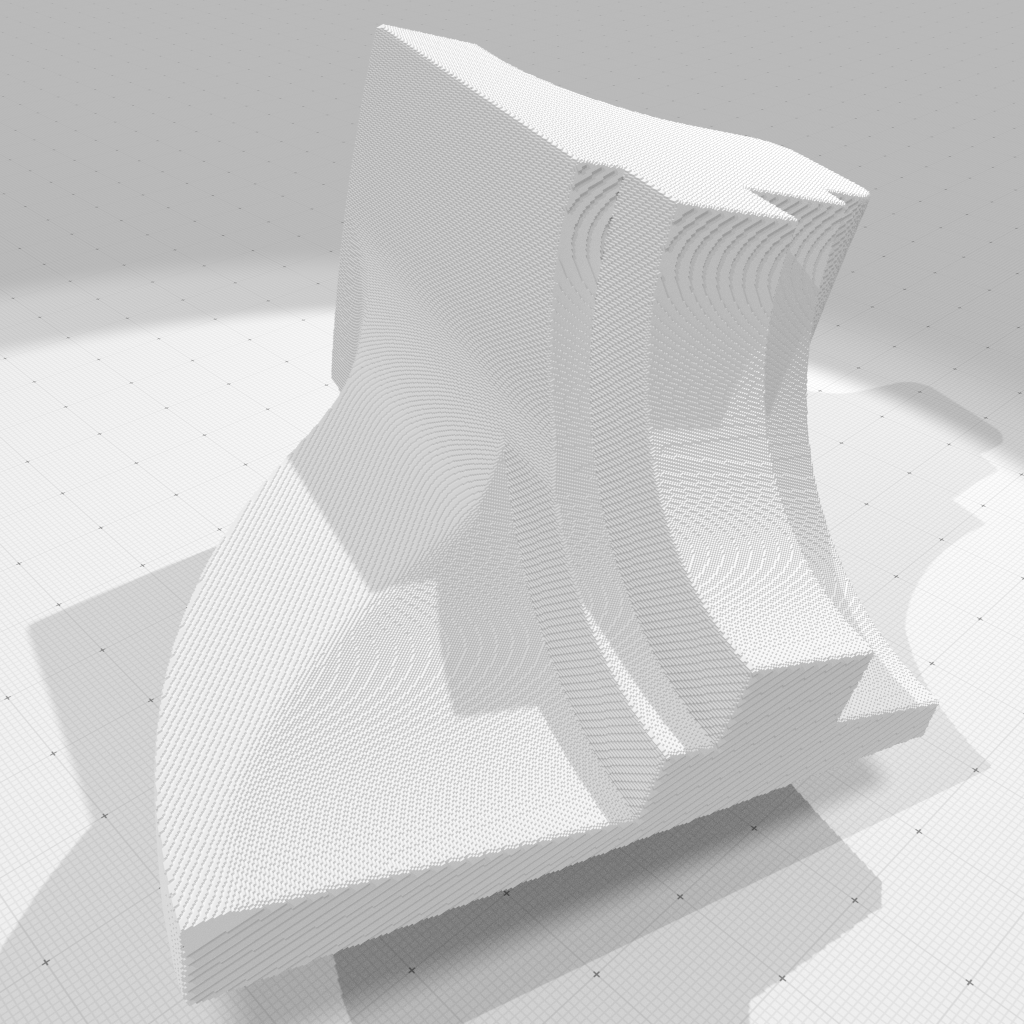
\includegraphics[width=4.0cm]{images/Feature/Fandisk} &
      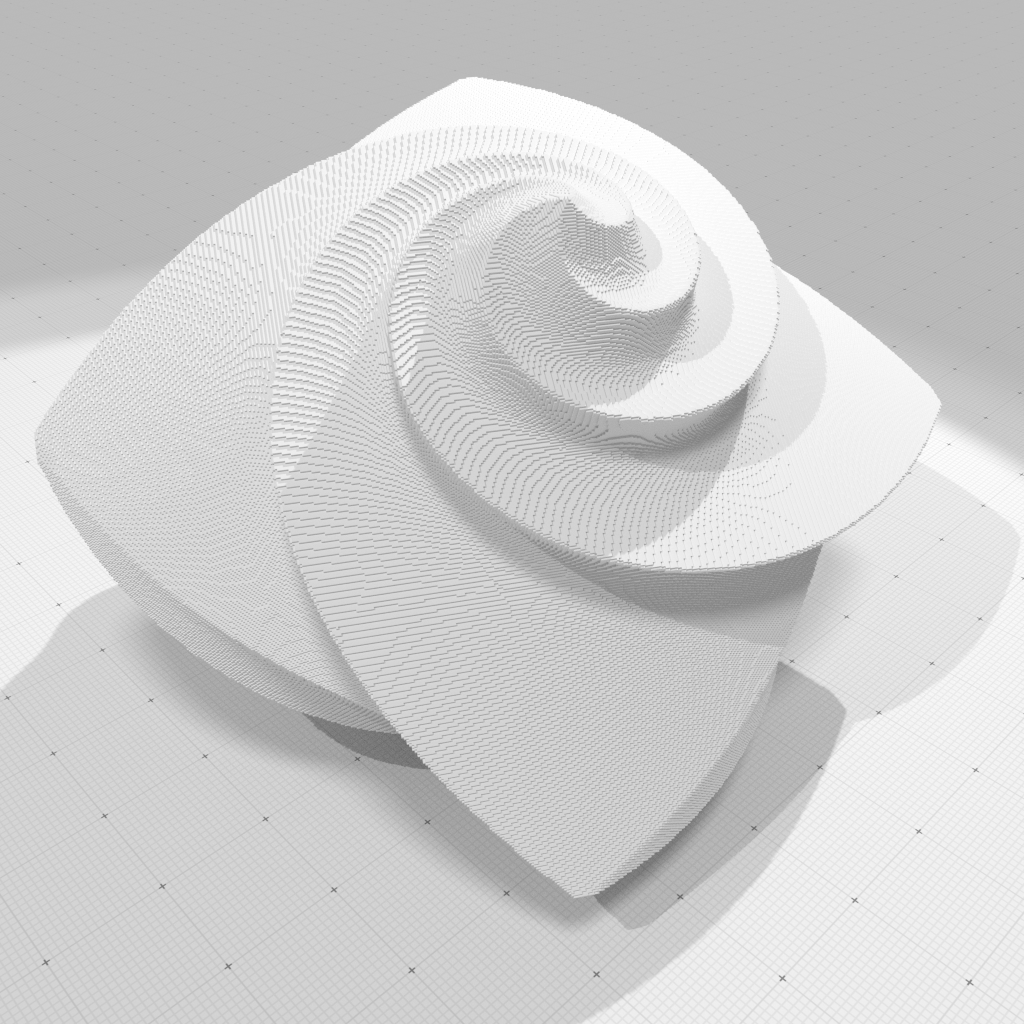
\includegraphics[width=4.0cm]{images/Feature/OctaFlower} &
       \\
      \rotatebox{90}{~\nauthors{Clarenz} $R_1$} &
      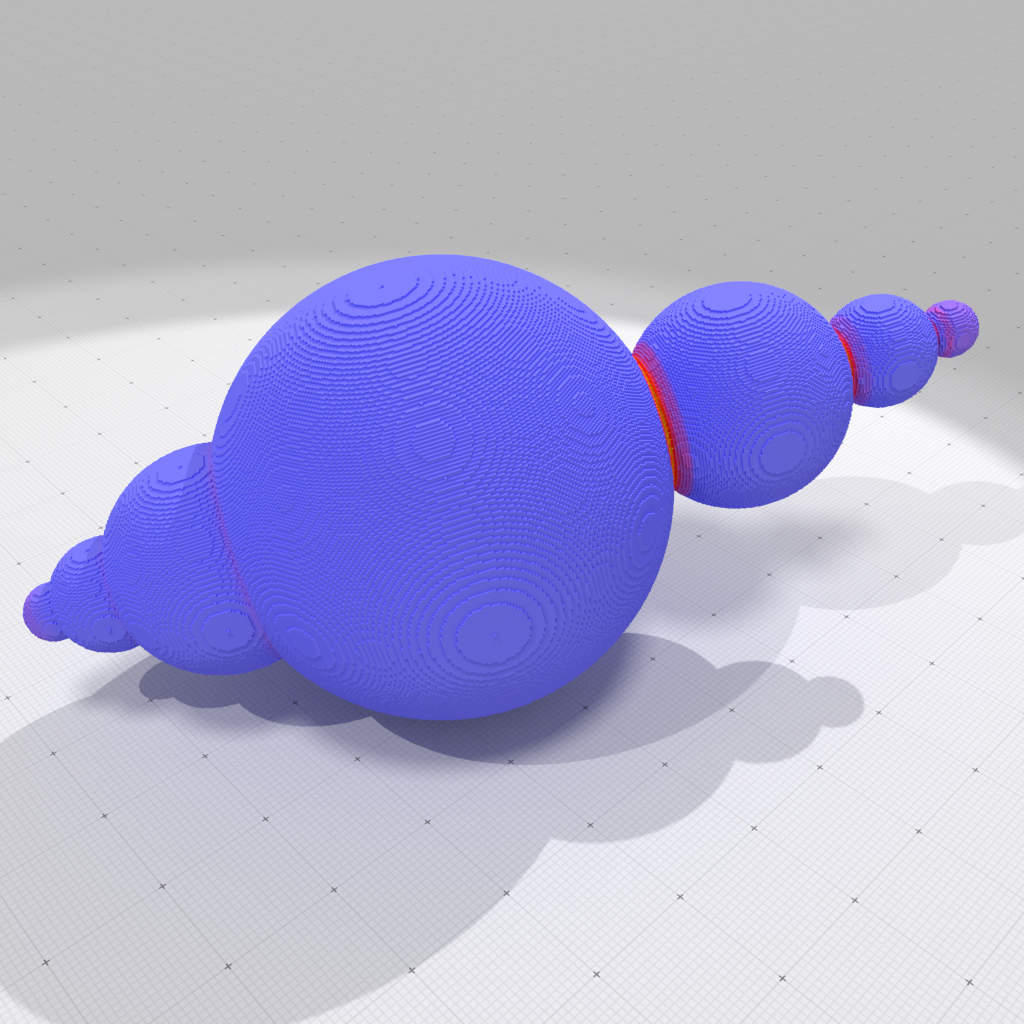
\includegraphics[width=4.0cm]{images/Feature/SphereSphereSphere_Moments_r_10_c1} &
      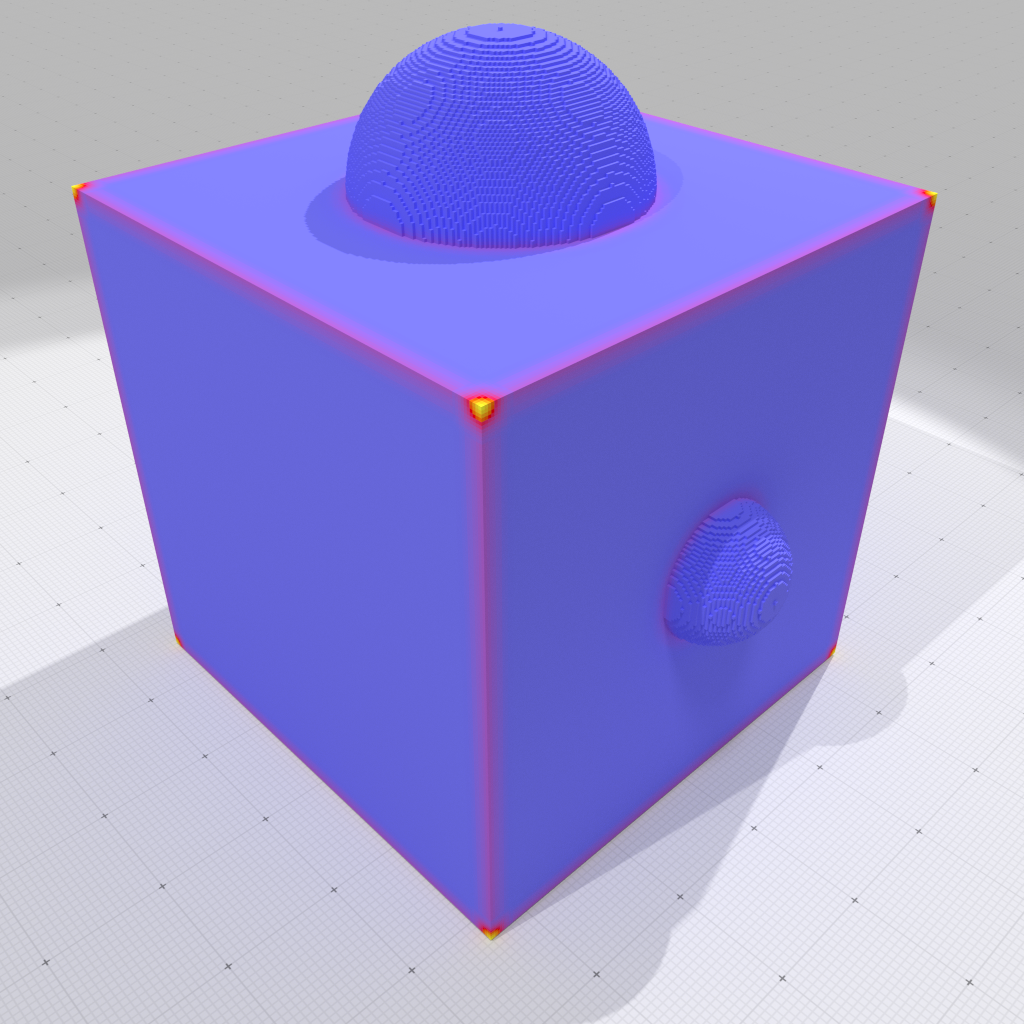
\includegraphics[width=4.0cm]{images/Feature/CubeSphere_Moments_r_10_c1} &
      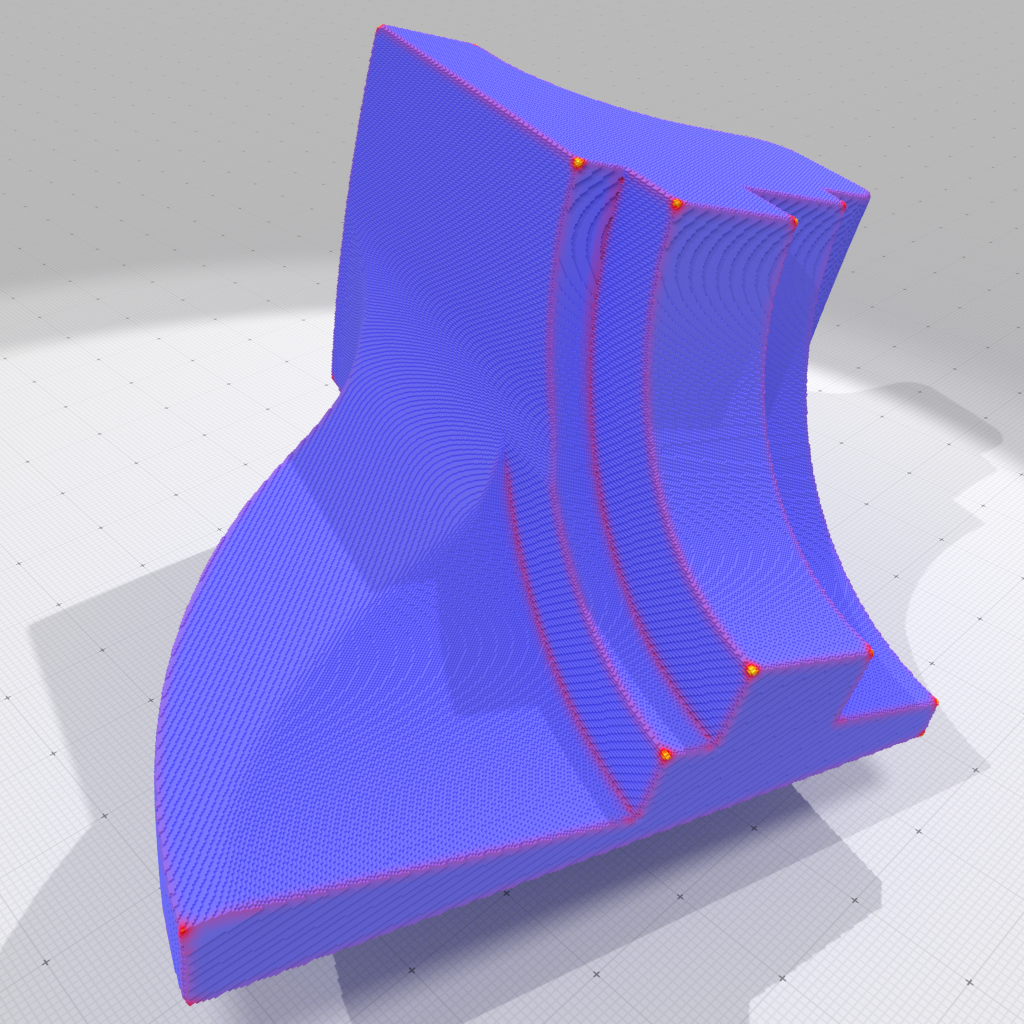
\includegraphics[width=4.0cm]{images/Feature/Fandisk_Moments_r_10_c1} &
      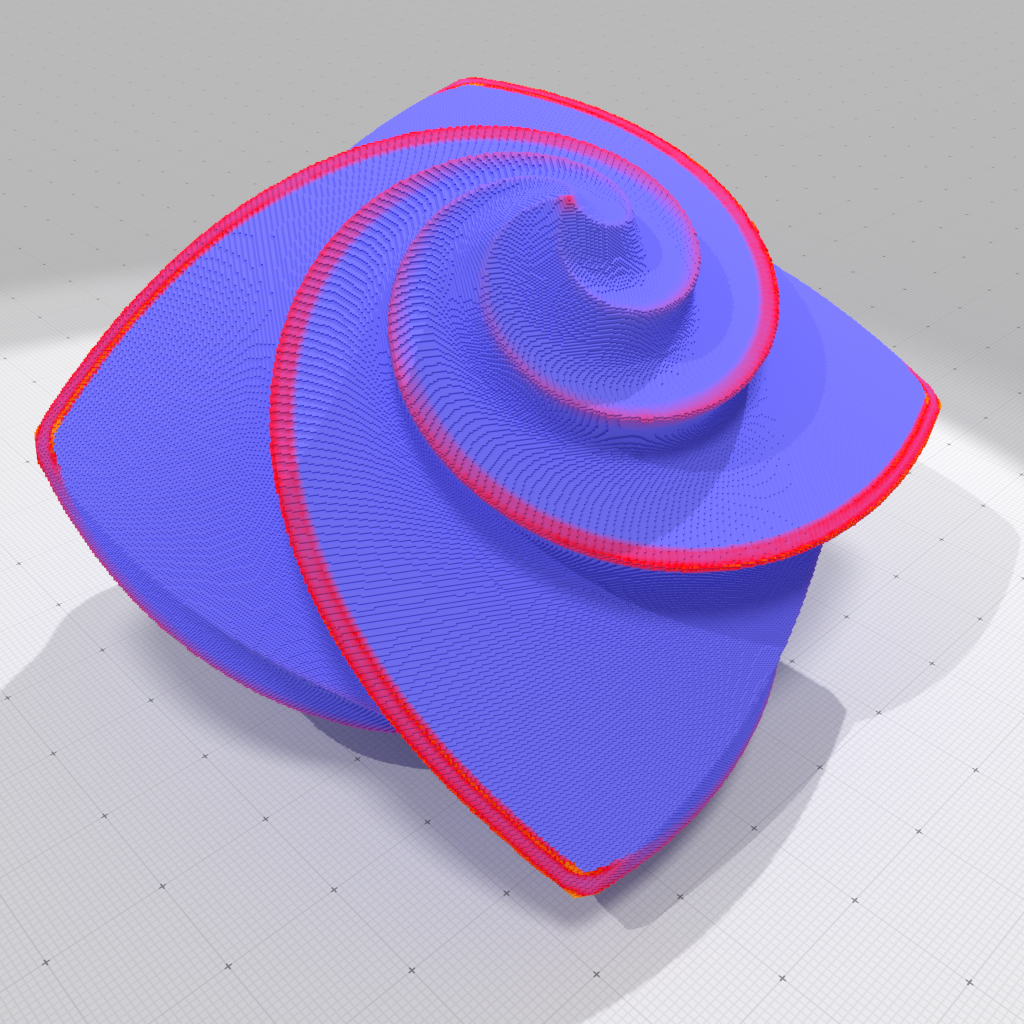
\includegraphics[width=4.0cm]{images/Feature/OctaFlower_512_Moments_r_10_c1} &
      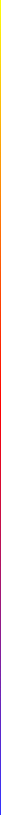
\includegraphics[width=0.1cm,height=4cm]{images/YMTB6W} \\
      \rotatebox{90}{~\nauthors{Clarenz} $R_2$} &
      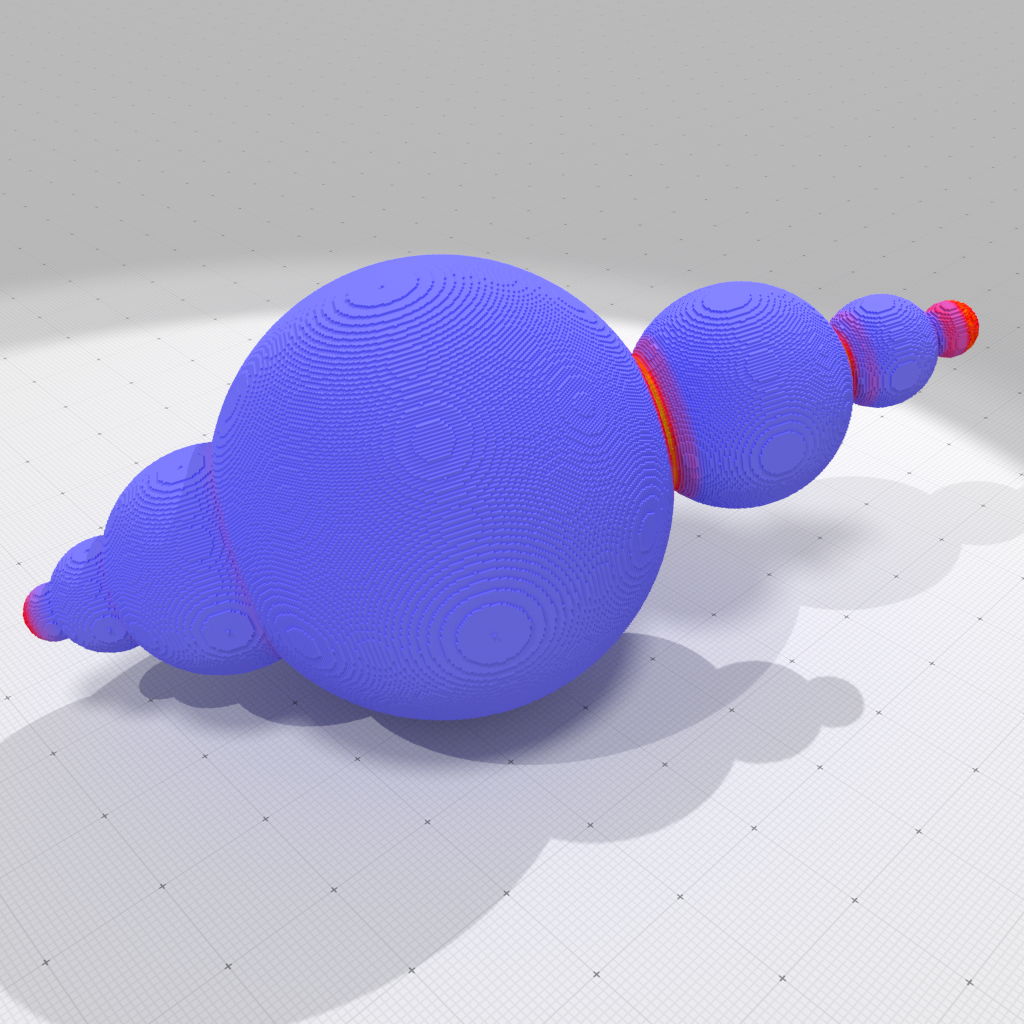
\includegraphics[width=4.0cm]{images/Feature/SphereSphereSphere_Moments_r_22_c1} &
      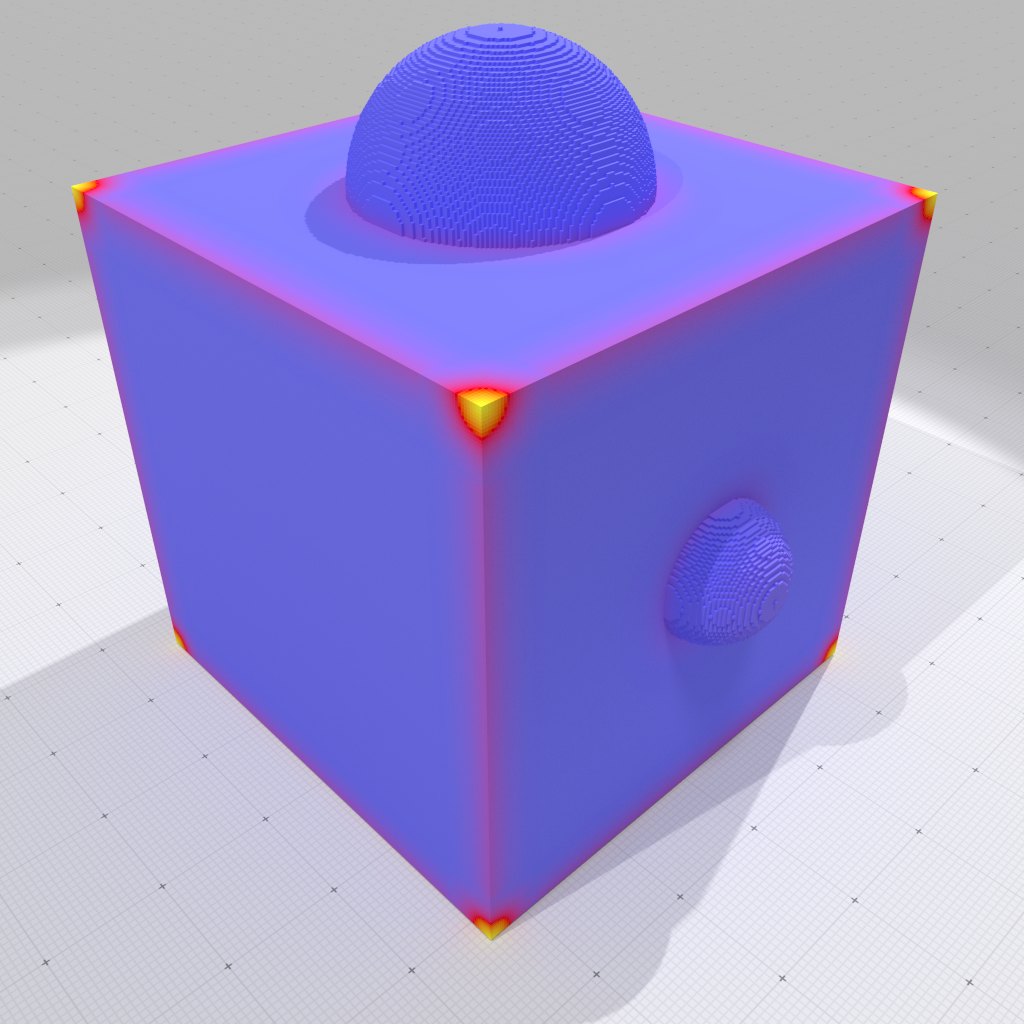
\includegraphics[width=4.0cm]{images/Feature/CubeSphere_Moments_r_22_c1} &
      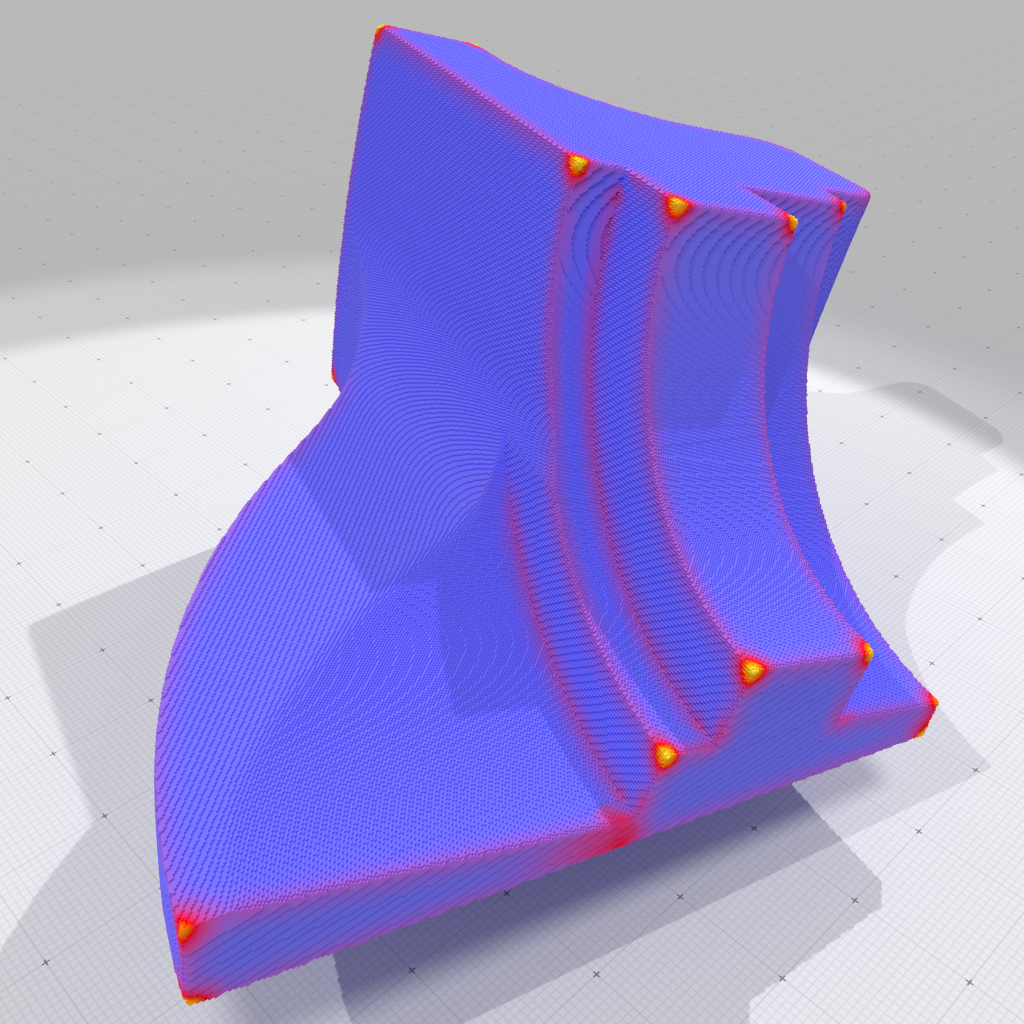
\includegraphics[width=4.0cm]{images/Feature/Fandisk_Moments_r_22_c1} &
      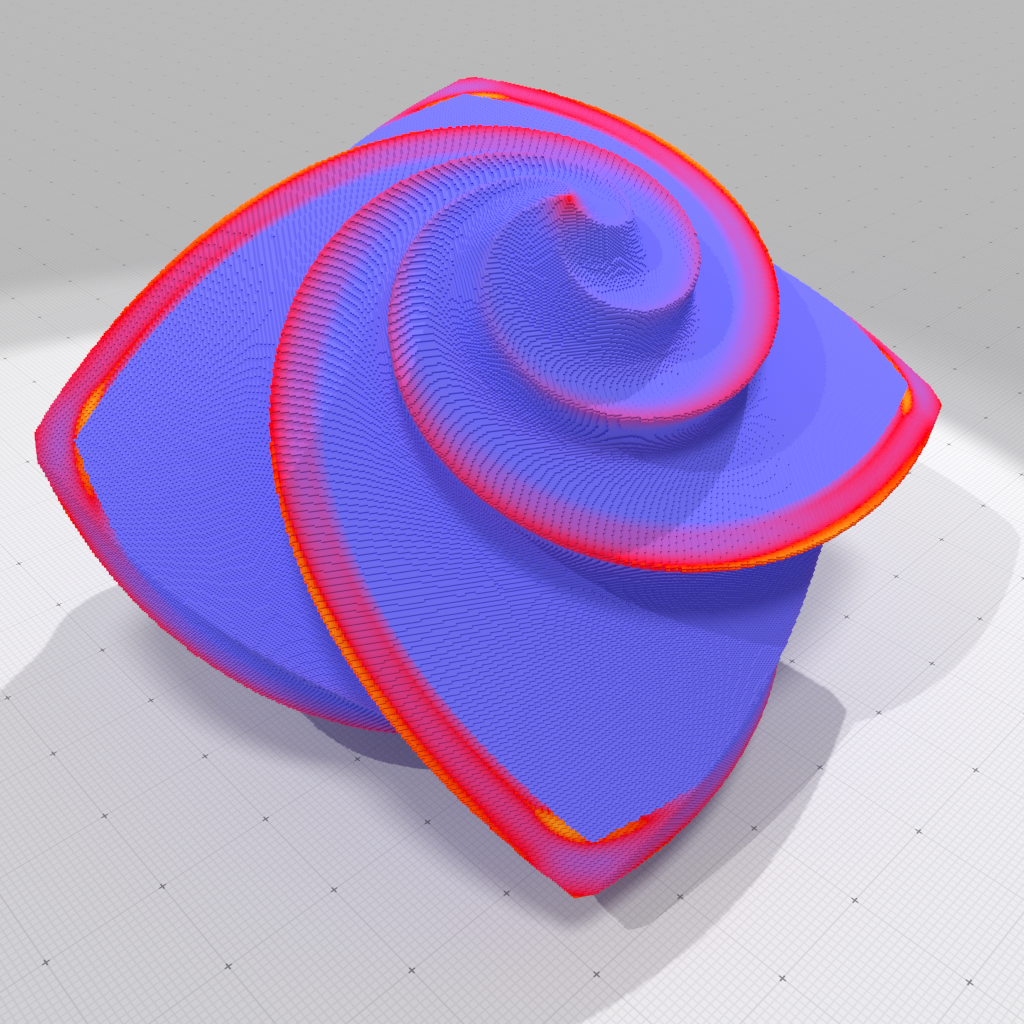
\includegraphics[width=4.0cm]{images/Feature/OctaFlower_512_Moments_r_22_c1} &
      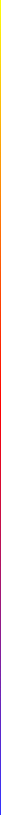
\includegraphics[width=0.1cm,height=4cm]{images/YMTB6W} \\
      \rotatebox{90}{~\nauthors{Mérigot} $R_1$, $r_1$} &
      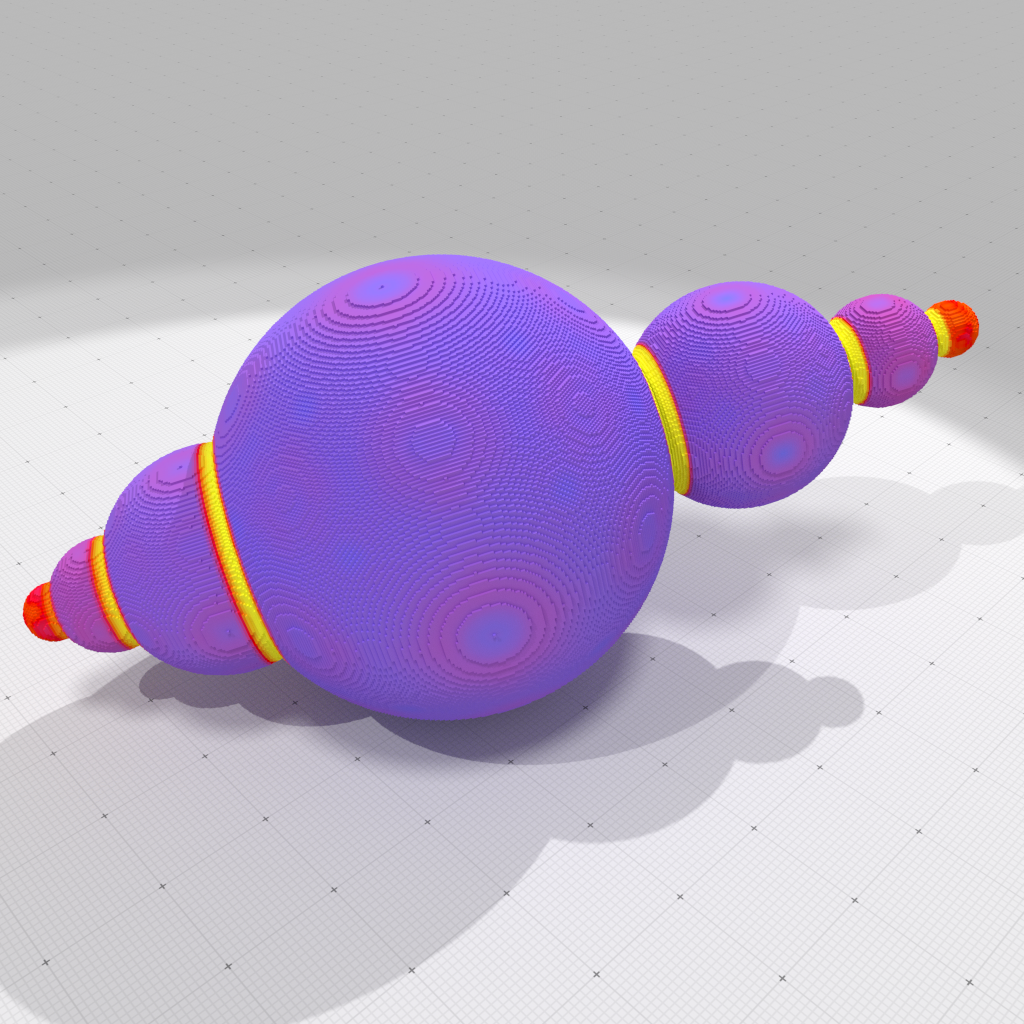
\includegraphics[width=4.0cm]{images/Feature/SphereSphereSphere_VCM_r_10} &
      \includegraphics[width=4.0cm]{images/Feature/CubeSphere_VCM_r_10} &
      \includegraphics[width=4.0cm]{images/Feature/Fandisk_VCM_r_10} &
      \includegraphics[width=4.0cm]{images/Feature/OctaFlower_512_VCM_r_10} &
      \includegraphics[width=0.1cm,height=4cm]{images/YMTB6W} \\
      \rotatebox{90}{~\nauthors{Mérigot} $R_2$, $r_2$} &
      \includegraphics[width=4.0cm]{images/Feature/SphereSphereSphere_VCM_r_22} &
      \includegraphics[width=4.0cm]{images/Feature/CubeSphere_VCM_r_22} &
      \includegraphics[width=4.0cm]{images/Feature/Fandisk_VCM_r_22} &
      \includegraphics[width=4.0cm]{images/Feature/OctaFlower_512_VCM_r_22} &
      \includegraphics[width=0.1cm,height=4cm]{images/YMTB6W}
    \end{tabular}%
  }
\end{overpic}
\caption[Évaluation des détecteurs de singularités sur des formes parfaitement discrétisées.]{Évaluation des détecteurs de singularités sur des formes parfaitement discrétisées.
\SpheresUnion : $400 \times 200 \times 200$ voxels, \CubeSphere : $200^3$ voxels, \Fandisk : $512^3$ voxels, \OctaFlower : $512^3$ voxels.
Paramètres utilisés pour \cauthors{Clarenz}{Telea2004}: $R_1 = 10$, $R_2 = 22$, $\alpha = 1$, $\beta = 50$.
Paramètres utilisés pour \cauthors{Mérigot}{Merigot2011}: $R_1 = 10$, $r_1 = 10$, $R_2 = 22$, $r_2 = 22$, $T = 0.2$.\label{fig:feature-comparative}}
\end{figure}


\begin{figure}[ht]
\begin{overpic}[width=\textwidth,height=.9\textheight]%
  {images/misc/TransparentPixel}
  \put(-5,50){%
    \setlength{\tabcolsep}{1pt}
    \begin{tabular}{l c c c cl}
      \rotatebox{90}{~~~~~~Input data} &
      \includegraphics[width=4.0cm]{images/Feature/SphereSphereSphere} &
      \includegraphics[width=4.0cm]{images/Feature/CubeSphere} &
      \includegraphics[width=4.0cm]{images/Feature/Fandisk} &
      \includegraphics[width=4.0cm]{images/Feature/OctaFlower} &
       \\
      \rotatebox{90}{~~~~~\nauthors{Mellado}} &
      \includegraphics[width=4.0cm]{images/Feature/SphereSphereSphere_Mellado_scale} &
      \includegraphics[width=4.0cm]{images/Feature/CubeSphere_Mellado_scale} &
      \includegraphics[width=4.0cm]{images/Feature/Fandisk_Mellado_scale} &
      \includegraphics[width=4.0cm]{images/Feature/OctaFlower_512_Mellado_scale} &
      \includegraphics[width=0.1cm,height=4cm]{images/YMTB6W} \\
      \rotatebox{90}{~~~~~~~~~\nauthors{Pauly}} &
      \includegraphics[width=4.0cm]{images/Feature/SphereSphereSphere_Pauly_scale} &
      \includegraphics[width=4.0cm]{images/Feature/CubeSphere_Pauly_scale} &
      \includegraphics[width=4.0cm]{images/Feature/Fandisk_Pauly_scale} &
      \includegraphics[width=4.0cm]{images/Feature/OctaFlower_512_Pauly_scale} &
      \includegraphics[width=0.1cm,height=4cm]{images/YMTB6W} \\
      \rotatebox{90}{~~~~~\nauthors{Park}} &
      \includegraphics[width=4.0cm]{images/Feature/SphereSphereSphere_Tensor_scale} &
      \includegraphics[width=4.0cm]{images/Feature/CubeSphere_Tensor_scale} &
      \includegraphics[width=4.0cm]{images/Feature/Fandisk_Tensor_scale} &
      \includegraphics[width=4.0cm]{images/Feature/OctaFlower_512_Tensor_scale} &
      \rotatebox{90}{\includegraphics[width=0.2cm]{images/Feature/Red} Feature~~~~\includegraphics[width=0.2cm]{images/Feature/Green} Non-feature} \\
      \rotatebox{90}{~~~~~~~~~~~Our} &
      \includegraphics[width=4.0cm]{images/Feature/SphereSphereSphere_II_scale} &
      \includegraphics[width=4.0cm]{images/Feature/CubeSphere_II_scale} &
      \includegraphics[width=4.0cm]{images/Feature/Fandisk_II_scale} &
      \includegraphics[width=4.0cm]{images/Feature/OctaFlower_512_II_scale} &
      \rotatebox{90}{\includegraphics[width=0.2cm]{images/Feature/Red} Edge~~\includegraphics[width=0.2cm]{images/Feature/Blue} Smooth~~\includegraphics[width=0.2cm]{images/Feature/Green} Flat}
    \end{tabular}
    }
    \end{overpic}
    \caption[Évaluation des détecteurs de singularités sur des formes parfaitement discrétisées.]{Évaluation des détecteurs de singularités sur des formes parfaitement discrétisées.
    \SpheresUnion : $400 \times 200 \times 200$ voxels, \CubeSphere : $200^3$ voxels, \Fandisk : $512^3$ voxels, \OctaFlower : $512^3$ voxels.
    Paramètres utilisés pour \cauthors{Mellado}{Mellado2012}: $r_{min} = 5$, $r_{max} = 25$.
    Paramètres utilisés pour \cauthors{Pauly}{Pauly2003}: $r_{min} = 5$, $r_{max} = 25$, $\tau_{max} = 0.01$.
    Paramètres utilisés pour \cauthors{Park}{Park2012}: $r_{min} = 5$, $r_{max} = 25$, $\omega_{min} = 1.4$, $\omega_{max} = 1.4$, $\tau = 1.2$.
    Paramètres utilisés pour notre algorithme : $r_{min} = 5$, $r_{max} = 25$.\label{fig:feature-comparative-2}}
\end{figure}

\begin{figure}[ht]
\begin{overpic}[width=\textwidth,height=.9\textheight]%
  {images/misc/TransparentPixel}
  \put(-5,50){%
    \setlength{\tabcolsep}{1pt}
    \begin{tabular}{l c c c cl}
      \rotatebox{90}{~~~~~~Input data} &
      \includegraphics[width=4.0cm]{images/Feature/SphereSphereSphere_noise2} &
      \includegraphics[width=4.0cm]{images/Feature/CubeSphere_noise2} &
      \includegraphics[width=4.0cm]{images/Feature/Fandisk_noise2} &
      \includegraphics[width=4.0cm]{images/Feature/OctaFlower_noise2} &
       \\
      \rotatebox{90}{~\nauthors{Clarenz} $R_1$} &
      \includegraphics[width=4.0cm]{images/Feature/SphereSphereSphere_noise_Moments_r_10_c1} &
      \includegraphics[width=4.0cm]{images/Feature/CubeSphere_noise_Moments_r_10_c1} &
      \includegraphics[width=4.0cm]{images/Feature/Fandisk_noise_Moments_r_10_c1} &
      \includegraphics[width=4.0cm]{images/Feature/OctaFlower_512_noise_Moments_r_10_c1} &
      \includegraphics[width=0.1cm,height=4cm]{images/YMTB6W} \\
      \rotatebox{90}{~\nauthors{Clarenz} $R_2$} &
      \includegraphics[width=4.0cm]{images/Feature/SphereSphereSphere_noise_Moments_r_22_c1} &
      \includegraphics[width=4.0cm]{images/Feature/CubeSphere_noise_Moments_r_22_c1} &
      \includegraphics[width=4.0cm]{images/Feature/Fandisk_noise_Moments_r_22_c1} &
      \includegraphics[width=4.0cm]{images/Feature/OctaFlower_512_noise_Moments_r_22_c1} &
      \includegraphics[width=0.1cm,height=4cm]{images/YMTB6W} \\
      \rotatebox{90}{~\nauthors{Mérigot} $R_1$,  $r_1$} &
      \includegraphics[width=4.0cm]{images/Feature/SphereSphereSphere_noise_VCM_r_10} &
      \includegraphics[width=4.0cm]{images/Feature/CubeSphere_noise_VCM_r_10} &
      \includegraphics[width=4.0cm]{images/Feature/Fandisk_noise_VCM_r_10} &
      \includegraphics[width=4.0cm]{images/Feature/OctaFlower_512_noise_VCM_r_10} &
      \includegraphics[width=0.1cm,height=4cm]{images/YMTB6W} \\
      \rotatebox{90}{~\nauthors{Mérigot} $R_2$, $r_2$} &
      \includegraphics[width=4.0cm]{images/Feature/SphereSphereSphere_noise_VCM_r_22} &
      \includegraphics[width=4.0cm]{images/Feature/CubeSphere_noise_VCM_r_22} &
      \includegraphics[width=4.0cm]{images/Feature/Fandisk_noise_VCM_r_22} &
      \includegraphics[width=4.0cm]{images/Feature/OctaFlower_512_noise_VCM_r_22} &
      \includegraphics[width=0.1cm,height=4cm]{images/YMTB6W}
    \end{tabular}
    }
    \end{overpic}
    \caption[Évaluation des détecteurs de singularités sur des approximations bruitées de \RefFigure{fig:feature-comparative}]{Évaluation des détecteurs de singularités sur des approximations bruitées de \RefFigure{fig:feature-comparative}.
    \SpheresUnion : $400 \times 200 \times 200$ voxels, \CubeSphere : $200^3$ voxels, \Fandisk : $512^3$ voxels, \OctaFlower : $512^3$ voxels.
    Paramètres utilisés pour \cauthors{Clarenz}{Telea2004}: $R_1 = 10$, $R_2 = 22$, $\alpha = 1$, $\beta = 50$.
    Paramètres utilisés pour \cauthors{Mérigot}{Merigot2011}: $R_1 = 10$, $r_1 = 10$, $R_2 = 22$, $r_2 = 22$, $T = 0.2$.\label{fig:feature-comparative-noise}}
\end{figure}

\begin{figure}[ht]
\begin{overpic}[width=\textwidth,height=.9\textheight]%
  {images/misc/TransparentPixel}
  \put(-5,50){%
    \setlength{\tabcolsep}{1pt}
    \begin{tabular}{l c c c c l}
      \rotatebox{90}{~~~~~~Input data} &
      \includegraphics[width=4.0cm]{images/Feature/SphereSphereSphere_noise2} &
      \includegraphics[width=4.0cm]{images/Feature/CubeSphere_noise2} &
      \includegraphics[width=4.0cm]{images/Feature/Fandisk_noise2} &
      \includegraphics[width=4.0cm]{images/Feature/OctaFlower_noise2} &
      \\
      \rotatebox{90}{~~~~~~\nauthors{Mellado}} &
      \includegraphics[width=4.0cm]{images/Feature/SphereSphereSphere_noise_Mellado_scale} &
      \includegraphics[width=4.0cm]{images/Feature/CubeSphere_noise_Mellado_scale} &
      \includegraphics[width=4.0cm]{images/Feature/Fandisk_noise_Mellado_scale} &
      \includegraphics[width=4.0cm]{images/Feature/OctaFlower_512_noise_Mellado_scale} &
      \includegraphics[width=0.1cm,height=4cm]{images/YMTB6W}
      \\
      \rotatebox{90}{~~~~~~~~~~\nauthors{Pauly}} &
      \includegraphics[width=4.0cm]{images/Feature/SphereSphereSphere_noise_Pauly_scale} &
      \includegraphics[width=4.0cm]{images/Feature/CubeSphere_noise_Pauly_scale} &
      \includegraphics[width=4.0cm]{images/Feature/Fandisk_noise_Pauly_scale} &
      \includegraphics[width=4.0cm]{images/Feature/OctaFlower_512_noise_Pauly_scale} &
      \includegraphics[width=0.1cm,height=4cm]{images/YMTB6W}
      \\
      \rotatebox{90}{~~~~~~\nauthors{Park}} &
      \includegraphics[width=4.0cm]{images/Feature/SphereSphereSphere_noise_Tensor_scale} &
      \includegraphics[width=4.0cm]{images/Feature/CubeSphere_noise_Tensor_scale} &
      \includegraphics[width=4.0cm]{images/Feature/Fandisk_noise_Tensor_scale} &
      \includegraphics[width=4.0cm]{images/Feature/OctaFlower_512_noise_Tensor_scale} &
      \rotatebox{90}{\includegraphics[width=0.2cm]{images/Feature/Red} Feature~~~~\includegraphics[width=0.2cm]{images/Feature/Green} Non-feature} \\
      \rotatebox{90}{~~~~~~~~~~~~Our} &
      \includegraphics[width=4.0cm]{images/Feature/SphereSphereSphere_noise_II_scale} &
      \includegraphics[width=4.0cm]{images/Feature/CubeSphere_noise_II_scale} &
      \includegraphics[width=4.0cm]{images/Feature/Fandisk_noise_II_scale} &
      \includegraphics[width=4.0cm]{images/Feature/OctaFlower_512_noise_II_scale} &
      \rotatebox{90}{\includegraphics[width=0.2cm]{images/Feature/Red} Edge~~\includegraphics[width=0.2cm]{images/Feature/Blue} Smooth~~\includegraphics[width=0.2cm]{images/Feature/Green} Flat}
    \end{tabular}
    }
    \end{overpic}
    \caption[Évaluation des détecteurs de singularités sur des approximations bruitées de \RefFigure{fig:feature-comparative-2}]{Évaluation des détecteurs de singularités sur des approximations bruitées de \RefFigure{fig:feature-comparative-2}.
    \SpheresUnion : $400 \times 200 \times 200$ voxels, \CubeSphere : $200^3$ voxels, \Fandisk : $512^3$ voxels, \OctaFlower : $512^3$ voxels.
    Paramètres utilisés pour \cauthors{Mellado}{Mellado2012}: $r_{min} = 5$, $r_{max} = 25$.
    Paramètres utilisés pour \cauthors{Pauly}{Pauly2003}: $r_{min} = 5$, $r_{max} = 25$, $\tau_{max} = 0.01$.
    Paramètres utilisés pour \cauthors{Park}{Park2012}: $r_{min} = 5$, $r_{max} = 25$, $\omega_{min} = 1.4$, $\omega_{max} = 1.4$, $\tau = 1.2$.
    Paramètres utilisés pour notre algorithme : $r_{min} = 5$, $r_{max} = 25$.\label{fig:feature-comparative-noise-2}}
\end{figure}

Les méthodes basées sur la variation de barycentres (\nauthor{Clarenz}) et \VCM
(\nauthor{Mérigot}) étant mono-échelles, nous avons choisi deux échelles
d'analyse (dans le même éventail que les estimateurs multi-échelles) afin de
montrer les problèmes du mono-échelle sur des objets ayant plusieurs niveaux de
lecture comme \CubeSphere ou \SpheresUnion.
%
\paragraph{}
%
La méthode de \nauthor{Clarenz} offre de très bons résultats. Comme espéré, les petits
rayons détectent les petites régions non-lisses (en rouge-jaune, se référer à la
carte des couleurs à droite des résultats) pendant que d'importants rayons renforcent
cette détection des régions non-lisses tout en considérant de petites zones
lisses comme non-lisses comme le montre l'objet \SpheresUnion. Le choix
des rayons --- et donc une étude à priori de la forme --- est alors important
pour la qualité des résultats obtenus. Notons toutefois que cet estimateur
semble assez robuste au bruit.
%
\paragraph{}
%
La méthode de \nauthor{Mérigot} offre également de bons résultats sur des
surfaces bruitées et non bruitées. Cependant cela nécessite trois paramètres qui
sont difficiles à déterminer pour une large catégorie de formes. Lorsque ceux-ci
sont sur-évalués, les zones caractéristiques détectées englobent les zones
proches non pertinentes comme c'est le cas avec le choix de $R_2$ et $r_2$ sur
la \RefFigure{fig:feature-comparative} par exemple.
%
\paragraph{}
%
La méthode de \nauthor{Mellado} semble quant à elle insensible au bruit, mais des artefacts
apparaissent sur les angles droits (voir les côtés de \CubeSphere par
exemple) à cause de l'utilisation de sphères.
%
\paragraph{}
%
La méthode de \nauthor{Pauly} fournit de bons résultats mais a tendance à considérer
des zones lisses à forte courbure comme des zones caractéristiques (comme la
plus petite sphère de \SpheresUnion, ce qui est logique puisque ce
détecteur est lié à la courbure de la forme. De plus, le choix du paramètre
$\tau_{max}$ est assez dépendant de la géométrie de la forme à analyser puisque
c'est cela qui va déterminer le seuil de courbure à partir de laquelle nous
considérons que nous sommes sur des zones caractéristiques. Enfin, cet
estimateur semble assez sensible au bruit puisqu'il collecte les informations de
courbure de manière surfacique.
%
\paragraph{}
%
La méthode de \nauthors{Park} requiert beaucoup de paramètres pour être fonctionnelle. De
nos expériences, $\omega^-$ et $\omega^+$ sont très dépendants de la géométrie de
la forme et de ce que nous considérons comme des zones caractéristiques. Aux
endroits de forte courbure, cette analyse détecte généralement les points
caractéristiques. Cependant, lorsque des singularités ont de faibles angles
diédraux, des mauvaises classifications apparaissent (sur la sphère de
\CubeSphere par exemple). Sur des données bruitées, avec les mêmes
paramètres $\omega^-$, $\omega^+$ et $\tau$, il ne détecte que les zones à très
forte courbure. Dans les faits, pour avoir de meilleurs résultats sur des
données bruitées, il faudrait changer les paramètres et donc étudier la forme à
analyser. Nous pouvons cependant noter que cette méthode permet une
classification, contrairement aux autres.
%
\paragraph{}
%
Tous les estimateurs vus précédemment n'arrivent pas à détecter toutes les zones
caractéristiques à différentes échelles, la principale difficulté est d'adapter
les paramètres pour détecter les petites régions tout en restant robuste au
bruit. Notre estimateur, en analysant la distance à tous les modèles linéaires
comme décrit dans le \RefSection{sec:applications:feature:II:classification},
permet de détecter et classifier les singularités (\featedge) des régions lisse
(\featsmooth) et des zones à courbure nulle (\featflat) indépendamment de leur
échelle. Ainsi, aucun paramètre mis à part l'ensemble de rayons n'est requis
(ce qui est également le cas pour les autres estimateurs comparés). Cependant,
il est importer de noter que le rayon maximal $R_0$ de notre ensemble de rayons
est relié à la plus petite courbure des régions lisses que nous souhaitons
détecter, comme nous l'avons vu précédemment.


Des zones autour des singularités sont parfois classifiées avec erreur
comme des régions \featsmooth (sur l'objet \CubeSphere par exemple). Cet
artefact est provoqué par la transition entre des parties \featflat et des
parties \featedge. Si nous analysons la transition, nous pouvons voir que la
courbure suit une courbe de pente $-1$ lorsqu'elle est au dessus de
$\CurvMax(R,h)$ (modèle \featedge) pour de grands rayons et a des valeurs au
dessous de $\CurvMax(R,h)$ pour de petits rayons (modèle \featflat). Entre ces
deux états, la courbure doit suivre des courbes de pente $0$ (modèle
\featsmooth) pour connecter les deux autres états. Cette transition peut être
prédominante sur des zones proches de zones caractéristiques \featedge. Cet
artefact peut être retiré facilement en mesurant la distance géométrique entre
un \featedge sur la surface, et reclasser les fausses zones \featsmooth vers
leur état avant la transition si la distance est petite.


Sur des objets bruités, notre classification continue de détecter avec
pertinence les zones \featedge, \featsmooth et \featflat, mais des artefacts
peuvent apparaître sur des régions lisses. Ceci est dû au fait que la fonction
$\DigFeatDD$ n'est plus une droite, mais plutôt une ligne polygonale. Cet artefact peut
être considéré soit par l'utilisation d'une meilleure distance aux modèles, soit
par suppression les petites régions \featedge (comme dans \cite{Park2012}). Il
faut rappeler que nous présentons ici les résultats sans post-traitement de
notre estimateur; il est alors clair que ces résultats peuvent être facilement
améliorés.
%
\subsection{Conclusion sur l'estimation de singularité}
%
Dans cette partie, nous avons défini un nouvel outil de détection de singularité
simple et robuste basé sur les estimateurs de courbure par intégration du
chapitre précédent. Celui-ci, défini en dimension 2 et 3 et s'appuyant sur les
bonnes propriétés mathématiques des estimateurs de courbure, propose de détecter
les parties non-$C^1$, les parties $C^3$ et les parties à courbure nulle sur la
surface d'objets digitaux. Puisque l'approche proposée est basée sur des
quantités locales différentielles à plusieurs échelles, la classification
obtenue est localement adaptative et invariante à l'échelle (au sens où elle
capture les singularités à différentes échelles sur le même objet géométrique).


Nous avons évalué expérimentalement ce détecteur avec des méthodes
représentatives de l'état de l'art et montré qu'il était très compétitif en
arrivant à détecter des singularités même à des échelles différentes sans autre
paramètre à choisir que l'ensemble de rayons. D'ailleurs, cet ensemble de
rayons constitue une limitation. Comme le rayon maximal de cet ensemble est
dépendant de la singularité maximale que nous souhaitons détecter, leur réglage
peut être important.


Enfin, comme pour les estimateurs de courbure, notre estimateur est basé sur
l'intégration volumique de la sphère et cette opération reste coûteuse et peut
la rendre moins compétitive face à d'autres à échelle fixe. Cependant, notre
méthode permet de détecter les singularités à plusieurs échelles ce qui est la
principale défaillance des autres méthodes à échelle fixe.
\clearpage
